\documentclass[twoside]{book}

% Packages required by doxygen
\usepackage{fixltx2e}
\usepackage{calc}
\usepackage{doxygen}
\usepackage[export]{adjustbox} % also loads graphicx
\usepackage{graphicx}
\usepackage[utf8]{inputenc}
\usepackage{makeidx}
\usepackage{multicol}
\usepackage{multirow}
\PassOptionsToPackage{warn}{textcomp}
\usepackage{textcomp}
\usepackage[nointegrals]{wasysym}
\usepackage[table]{xcolor}

% Font selection
\usepackage[T1]{fontenc}
\usepackage[scaled=.90]{helvet}
\usepackage{courier}
\usepackage{amssymb}
\usepackage{sectsty}
\renewcommand{\familydefault}{\sfdefault}
\allsectionsfont{%
  \fontseries{bc}\selectfont%
  \color{darkgray}%
}
\renewcommand{\DoxyLabelFont}{%
  \fontseries{bc}\selectfont%
  \color{darkgray}%
}
\newcommand{\+}{\discretionary{\mbox{\scriptsize$\hookleftarrow$}}{}{}}

% Page & text layout
\usepackage{geometry}
\geometry{%
  a4paper,%
  top=2.5cm,%
  bottom=2.5cm,%
  left=2.5cm,%
  right=2.5cm%
}
\tolerance=750
\hfuzz=15pt
\hbadness=750
\setlength{\emergencystretch}{15pt}
\setlength{\parindent}{0cm}
\setlength{\parskip}{0.2cm}
\makeatletter
\renewcommand{\paragraph}{%
  \@startsection{paragraph}{4}{0ex}{-1.0ex}{1.0ex}{%
    \normalfont\normalsize\bfseries\SS@parafont%
  }%
}
\renewcommand{\subparagraph}{%
  \@startsection{subparagraph}{5}{0ex}{-1.0ex}{1.0ex}{%
    \normalfont\normalsize\bfseries\SS@subparafont%
  }%
}
\makeatother

% Headers & footers
\usepackage{fancyhdr}
\pagestyle{fancyplain}
\fancyhead[LE]{\fancyplain{}{\bfseries\thepage}}
\fancyhead[CE]{\fancyplain{}{}}
\fancyhead[RE]{\fancyplain{}{\bfseries\leftmark}}
\fancyhead[LO]{\fancyplain{}{\bfseries\rightmark}}
\fancyhead[CO]{\fancyplain{}{}}
\fancyhead[RO]{\fancyplain{}{\bfseries\thepage}}
\fancyfoot[LE]{\fancyplain{}{}}
\fancyfoot[CE]{\fancyplain{}{}}
\fancyfoot[RE]{\fancyplain{}{\bfseries\scriptsize Generated on Wed Mar 23 2016 15\+:12\+:18 for Leaf\+G\+P by Doxygen }}
\fancyfoot[LO]{\fancyplain{}{\bfseries\scriptsize Generated on Wed Mar 23 2016 15\+:12\+:18 for Leaf\+G\+P by Doxygen }}
\fancyfoot[CO]{\fancyplain{}{}}
\fancyfoot[RO]{\fancyplain{}{}}
\renewcommand{\footrulewidth}{0.4pt}
\renewcommand{\chaptermark}[1]{%
  \markboth{#1}{}%
}
\renewcommand{\sectionmark}[1]{%
  \markright{\thesection\ #1}%
}

% Indices & bibliography
\usepackage{natbib}
\usepackage[titles]{tocloft}
\setcounter{tocdepth}{3}
\setcounter{secnumdepth}{5}
\makeindex

% Hyperlinks (required, but should be loaded last)
\usepackage{ifpdf}
\ifpdf
  \usepackage[pdftex,pagebackref=true]{hyperref}
\else
  \usepackage[ps2pdf,pagebackref=true]{hyperref}
\fi
\hypersetup{%
  colorlinks=true,%
  linkcolor=blue,%
  citecolor=blue,%
  unicode%
}

% Custom commands
\newcommand{\clearemptydoublepage}{%
  \newpage{\pagestyle{empty}\cleardoublepage}%
}


%===== C O N T E N T S =====

\begin{document}

% Titlepage & ToC
\hypersetup{pageanchor=false,
             bookmarks=true,
             bookmarksnumbered=true,
             pdfencoding=unicode
            }
\pagenumbering{roman}
\begin{titlepage}
\vspace*{7cm}
\begin{center}%
{\Large Leaf\+G\+P \\[1ex]\large 1.\+0 }\\
\vspace*{1cm}
{\large Generated by Doxygen 1.8.9.1}\\
\vspace*{0.5cm}
{\small Wed Mar 23 2016 15:12:18}\\
\end{center}
\end{titlepage}
\clearemptydoublepage
\tableofcontents
\clearemptydoublepage
\pagenumbering{arabic}
\hypersetup{pageanchor=true}

%--- Begin generated contents ---
\chapter{B\+E\+A\+G\+L\+E Puppy Reference Manual}
\label{index}\hypertarget{index}{}If you are new to B\+E\+A\+G\+L\+E \hyperlink{namespacePuppy}{Puppy}, start by browsing the \href{modules.html}{\tt modules}, especially the examples modules.

If you are looking for informations on specific element of the B\+E\+A\+G\+L\+E \hyperlink{namespacePuppy}{Puppy} framework, you can either check in the \href{annotated.html}{\tt compound list} for a specific class, or the \href{functions.html}{\tt compound member index} for a specific method. 
\chapter{Module Index}
\section{Modules}
Here is a list of all modules\+:\begin{DoxyCompactList}
\item \contentsline{section}{B\+E\+A\+G\+L\+E Puppy Library}{\pageref{group__Puppy}}{}
\end{DoxyCompactList}

\chapter{Namespace Index}
\section{Namespace List}
Here is a list of all documented namespaces with brief descriptions\+:\begin{DoxyCompactList}
\item\contentsline{section}{\hyperlink{namespacePuppy}{Puppy} \\*Namespace of all B\+E\+A\+G\+L\+E \hyperlink{namespacePuppy}{Puppy} G\+P framework classes and global functions }{\pageref{namespacePuppy}}{}
\end{DoxyCompactList}

\chapter{Hierarchical Index}
\section{Class Hierarchy}
This inheritance list is sorted roughly, but not completely, alphabetically\+:\begin{DoxyCompactList}
\item \contentsline{section}{Puppy\+:\+:Context}{\pageref{classPuppy_1_1Context}}{}
\item \contentsline{section}{Worker\+:\+:fitnessdata}{\pageref{structWorker_1_1fitnessdata}}{}
\item Function\begin{DoxyCompactList}
\item \contentsline{section}{Rosenbrock}{\pageref{classRosenbrock}}{}
\end{DoxyCompactList}
\item \contentsline{section}{Matrix}{\pageref{classMatrix}}{}
\item \contentsline{section}{Puppy\+:\+:Node}{\pageref{structPuppy_1_1Node}}{}
\item \contentsline{section}{Worker\+:\+:One\+Tree}{\pageref{structWorker_1_1OneTree}}{}
\item \contentsline{section}{Puppy\+:\+:Primitive}{\pageref{classPuppy_1_1Primitive}}{}
\begin{DoxyCompactList}
\item \contentsline{section}{Add}{\pageref{classAdd}}{}
\item \contentsline{section}{Cos}{\pageref{classCos}}{}
\item \contentsline{section}{Divide}{\pageref{classDivide}}{}
\item \contentsline{section}{Ephemeral}{\pageref{classEphemeral}}{}
\item \contentsline{section}{Exp}{\pageref{classExp}}{}
\item \contentsline{section}{Log}{\pageref{classLog}}{}
\item \contentsline{section}{Multiply}{\pageref{classMultiply}}{}
\item \contentsline{section}{Puppy\+:\+:Token\+T$<$ T $>$}{\pageref{classPuppy_1_1TokenT}}{}
\item \contentsline{section}{Sin}{\pageref{classSin}}{}
\item \contentsline{section}{Subtract}{\pageref{classSubtract}}{}
\end{DoxyCompactList}
\item \contentsline{section}{Puppy\+:\+:Primitive\+Handle}{\pageref{classPuppy_1_1PrimitiveHandle}}{}
\item Q\+Dialog\begin{DoxyCompactList}
\item \contentsline{section}{aboutwindow}{\pageref{classaboutwindow}}{}
\end{DoxyCompactList}
\item Q\+Graphics\+Item\begin{DoxyCompactList}
\item \contentsline{section}{Edge}{\pageref{classEdge}}{}
\item \contentsline{section}{Node}{\pageref{classNode}}{}
\end{DoxyCompactList}
\item Q\+Main\+Window\begin{DoxyCompactList}
\item \contentsline{section}{Main\+Window}{\pageref{classMainWindow}}{}
\end{DoxyCompactList}
\item Q\+Object\begin{DoxyCompactList}
\item \contentsline{section}{Worker}{\pageref{classWorker}}{}
\end{DoxyCompactList}
\item \contentsline{section}{Puppy\+:\+:Randomizer}{\pageref{classPuppy_1_1Randomizer}}{}
\item \contentsline{section}{Worker\+:\+:Stats}{\pageref{structWorker_1_1Stats}}{}
\item \contentsline{section}{Worker\+:\+:Tree\+Container}{\pageref{structWorker_1_1TreeContainer}}{}
\item \contentsline{section}{Worker\+:\+:Tree\+Struct}{\pageref{structWorker_1_1TreeStruct}}{}
\item vector\begin{DoxyCompactList}
\item \contentsline{section}{Puppy\+:\+:Tree}{\pageref{classPuppy_1_1Tree}}{}
\end{DoxyCompactList}
\end{DoxyCompactList}

\chapter{Class Index}
\section{Class List}
Here are the classes, structs, unions and interfaces with brief descriptions\+:\begin{DoxyCompactList}
\item\contentsline{section}{\hyperlink{classaboutwindow}{aboutwindow} }{\pageref{classaboutwindow}}{}
\item\contentsline{section}{\hyperlink{classAdd}{Add} \\*\hyperlink{classAdd}{Add} two doubles G\+P primitive }{\pageref{classAdd}}{}
\item\contentsline{section}{\hyperlink{classPuppy_1_1Context}{Puppy\+::\+Context} \\*Evolutionary context.

The evolutionary context includes the execution context used when interpreting the trees along with the problem set-\/up defined with the function and terminal set, and the randomizer }{\pageref{classPuppy_1_1Context}}{}
\item\contentsline{section}{\hyperlink{classCos}{Cos} }{\pageref{classCos}}{}
\item\contentsline{section}{\hyperlink{classDivide}{Divide} \\*Protected division of two doubles G\+P primitive }{\pageref{classDivide}}{}
\item\contentsline{section}{\hyperlink{classEdge}{Edge} }{\pageref{classEdge}}{}
\item\contentsline{section}{\hyperlink{classEphemeral}{Ephemeral} \\*\hyperlink{classEphemeral}{Ephemeral} random constant }{\pageref{classEphemeral}}{}
\item\contentsline{section}{\hyperlink{classExp}{Exp} }{\pageref{classExp}}{}
\item\contentsline{section}{\hyperlink{structWorker_1_1fitnessdata}{Worker\+::fitnessdata} }{\pageref{structWorker_1_1fitnessdata}}{}
\item\contentsline{section}{\hyperlink{classLog}{Log} }{\pageref{classLog}}{}
\item\contentsline{section}{\hyperlink{classMainWindow}{Main\+Window} }{\pageref{classMainWindow}}{}
\item\contentsline{section}{\hyperlink{classMatrix}{Matrix} }{\pageref{classMatrix}}{}
\item\contentsline{section}{\hyperlink{classMultiply}{Multiply} \\*\hyperlink{classMultiply}{Multiply} two doubles G\+P primitive }{\pageref{classMultiply}}{}
\item\contentsline{section}{\hyperlink{structPuppy_1_1Node}{Puppy\+::\+Node} \\*G\+P tree node structure }{\pageref{structPuppy_1_1Node}}{}
\item\contentsline{section}{\hyperlink{classNode}{Node} }{\pageref{classNode}}{}
\item\contentsline{section}{\hyperlink{structWorker_1_1OneTree}{Worker\+::\+One\+Tree} }{\pageref{structWorker_1_1OneTree}}{}
\item\contentsline{section}{\hyperlink{classPuppy_1_1Primitive}{Puppy\+::\+Primitive} \\*Genetic programming abstract primitive class.

A primitive is an abstract class of terminals and functions that can be used in a G\+P program. Concrete primitives must define method execute, which define the characteristic operation to execute. Primitives are generally heap allocated (with a call to the new operator) and managed by the associated smart pointer defined in class \hyperlink{classPuppy_1_1PrimitiveHandle}{Primitive\+Handle} }{\pageref{classPuppy_1_1Primitive}}{}
\item\contentsline{section}{\hyperlink{classPuppy_1_1PrimitiveHandle}{Puppy\+::\+Primitive\+Handle} \\*Smart pointer to a primitive.

\hyperlink{classPuppy_1_1Primitive}{Primitive} handle defines a smart pointer to a primitive. It behaves much like a standard pointer, but it also call the appriate refer and unrefer methods of class primitive }{\pageref{classPuppy_1_1PrimitiveHandle}}{}
\item\contentsline{section}{\hyperlink{classPuppy_1_1Randomizer}{Puppy\+::\+Randomizer} \\*Random number generator. C++ wrapper over standard C rand and srand functions }{\pageref{classPuppy_1_1Randomizer}}{}
\item\contentsline{section}{\hyperlink{classRosenbrock}{Rosenbrock} }{\pageref{classRosenbrock}}{}
\item\contentsline{section}{\hyperlink{classSin}{Sin} }{\pageref{classSin}}{}
\item\contentsline{section}{\hyperlink{structWorker_1_1Stats}{Worker\+::\+Stats} }{\pageref{structWorker_1_1Stats}}{}
\item\contentsline{section}{\hyperlink{classSubtract}{Subtract} \\*\hyperlink{classSubtract}{Subtract} two doubles G\+P primitive }{\pageref{classSubtract}}{}
\item\contentsline{section}{\hyperlink{classPuppy_1_1TokenT}{Puppy\+::\+Token\+T$<$ T $>$} \\*Token template, to use as variable terminal primitive }{\pageref{classPuppy_1_1TokenT}}{}
\item\contentsline{section}{\hyperlink{classPuppy_1_1Tree}{Puppy\+::\+Tree} \\*G\+P tree class.

The evolutionary context includes the execution context used when interpreting the trees along with the problem set-\/up defined with the function and terminal set, and the randomizer }{\pageref{classPuppy_1_1Tree}}{}
\item\contentsline{section}{\hyperlink{structWorker_1_1TreeContainer}{Worker\+::\+Tree\+Container} }{\pageref{structWorker_1_1TreeContainer}}{}
\item\contentsline{section}{\hyperlink{structWorker_1_1TreeStruct}{Worker\+::\+Tree\+Struct} }{\pageref{structWorker_1_1TreeStruct}}{}
\item\contentsline{section}{\hyperlink{classWorker}{Worker} }{\pageref{classWorker}}{}
\end{DoxyCompactList}

\chapter{Module Documentation}
\hypertarget{group__Puppy}{}\section{B\+E\+A\+G\+L\+E Puppy Library}
\label{group__Puppy}\index{B\+E\+A\+G\+L\+E Puppy Library@{B\+E\+A\+G\+L\+E Puppy Library}}


Classes and functions related B\+E\+A\+G\+L\+E \hyperlink{namespacePuppy}{Puppy} core mechanisms.  


\subsection*{Classes}
\begin{DoxyCompactItemize}
\item 
class \hyperlink{classPuppy_1_1Context}{Puppy\+::\+Context}
\begin{DoxyCompactList}\small\item\em Evolutionary context.

The evolutionary context includes the execution context used when interpreting the trees along with the problem set-\/up defined with the function and terminal set, and the randomizer. \end{DoxyCompactList}\item 
class \hyperlink{classPuppy_1_1Primitive}{Puppy\+::\+Primitive}
\begin{DoxyCompactList}\small\item\em Genetic programming abstract primitive class.

A primitive is an abstract class of terminals and functions that can be used in a G\+P program. Concrete primitives must define method execute, which define the characteristic operation to execute. Primitives are generally heap allocated (with a call to the new operator) and managed by the associated smart pointer defined in class \hyperlink{classPuppy_1_1PrimitiveHandle}{Primitive\+Handle}. \end{DoxyCompactList}\item 
class \hyperlink{classPuppy_1_1PrimitiveHandle}{Puppy\+::\+Primitive\+Handle}
\begin{DoxyCompactList}\small\item\em Smart pointer to a primitive.

\hyperlink{classPuppy_1_1Primitive}{Primitive} handle defines a smart pointer to a primitive. It behaves much like a standard pointer, but it also call the appriate refer and unrefer methods of class primitive. \end{DoxyCompactList}\item 
class \hyperlink{classPuppy_1_1Randomizer}{Puppy\+::\+Randomizer}
\begin{DoxyCompactList}\small\item\em Random number generator. C++ wrapper over standard C rand and srand functions. \end{DoxyCompactList}\item 
class \hyperlink{classPuppy_1_1TokenT}{Puppy\+::\+Token\+T$<$ T $>$}
\begin{DoxyCompactList}\small\item\em Token template, to use as variable terminal primitive. \end{DoxyCompactList}\item 
struct \hyperlink{structPuppy_1_1Node}{Puppy\+::\+Node}
\begin{DoxyCompactList}\small\item\em G\+P tree node structure. \end{DoxyCompactList}\item 
class \hyperlink{classPuppy_1_1Tree}{Puppy\+::\+Tree}
\begin{DoxyCompactList}\small\item\em G\+P tree class.

The evolutionary context includes the execution context used when interpreting the trees along with the problem set-\/up defined with the function and terminal set, and the randomizer. \end{DoxyCompactList}\end{DoxyCompactItemize}
\subsection*{Functions}
\begin{DoxyCompactItemize}
\item 
void \hyperlink{group__Puppy_gaaef144c802e721c9f3ef0a53b8728d3d}{Puppy\+::calculate\+Stats} (const std\+::vector$<$ Tree $>$ \&in\+Population, unsigned int in\+Generation, Q\+String \&io\+O\+S, double \&best\+\_\+fit, int \&best\+\_\+index, double \&avg\+Size, double \&max\+Size, double \&min\+Size)
\begin{DoxyCompactList}\small\item\em Calculate statistics for the actual population and display results to output stream. \end{DoxyCompactList}\item 
void \hyperlink{group__Puppy_ga3ae29733ace7314f669f288e6f2d4a8d}{Puppy\+::apply\+Crossover} (std\+::vector$<$ Tree $>$ \&io\+Population, Context \&io\+Context, float in\+Mating\+Proba=0.\+9, float in\+Distrib\+Proba=0.\+9, unsigned int in\+Max\+Tree\+Depth=17)
\begin{DoxyCompactList}\small\item\em Apply sub-\/tree crossover operation on a population of G\+P trees. \end{DoxyCompactList}\item 
void \hyperlink{group__Puppy_gac9ce564e7c3a601bc7cb9f39def4cfc4}{Puppy\+::exchange\+Sub\+Trees} (Tree \&io\+Tree1, unsigned int in\+Node1, const std\+::vector$<$ unsigned int $>$ \&in\+Stack1, Tree \&io\+Tree2, unsigned int in\+Node2, const std\+::vector$<$ unsigned int $>$ \&in\+Stack2)
\begin{DoxyCompactList}\small\item\em Exchange two sub-\/trees. \end{DoxyCompactList}\item 
void \hyperlink{group__Puppy_gae78df624fa96e33eaf9896ae00ea13cd}{Puppy\+::mate\+Trees} (Tree \&io\+Tree1, Tree \&io\+Tree2, Context \&io\+Context, float in\+Distrib\+Proba=0.\+9, unsigned int in\+Max\+Tree\+Depth=17)
\begin{DoxyCompactList}\small\item\em Mate two G\+P trees for crossover. \end{DoxyCompactList}\item 
void \hyperlink{group__Puppy_ga965ce68758651c3b9cf03db03799f709}{Puppy\+::initialize\+Population} (std\+::vector$<$ Tree $>$ \&io\+Population, Context \&io\+Context, float in\+Init\+Grow\+Proba=0.\+5, unsigned int in\+Min\+Depth=2, unsigned int in\+Max\+Depth=5)
\begin{DoxyCompactList}\small\item\em Initialize ramped half-\/and-\/half a population of G\+P trees. \end{DoxyCompactList}\item 
unsigned int \hyperlink{group__Puppy_ga0039778b0dbe47bcf5889d6587f75536}{Puppy\+::initialize\+Tree\+Full} (Tree \&io\+Tree, Context \&io\+Context, unsigned int in\+Depth)
\begin{DoxyCompactList}\small\item\em Initialize a G\+P tree with full approach. \end{DoxyCompactList}\item 
unsigned int \hyperlink{group__Puppy_gac4bc47167b30efa18c41f039b00d4b66}{Puppy\+::initialize\+Tree\+Grow} (Tree \&io\+Tree, Context \&io\+Context, unsigned int in\+Min\+Depth, unsigned int in\+Max\+Depth)
\begin{DoxyCompactList}\small\item\em Initialize a G\+P tree with grow approach. \end{DoxyCompactList}\item 
void \hyperlink{group__Puppy_gae96197fb941007acd222f578815270ff}{Puppy\+::apply\+Mutation\+Standard} (std\+::vector$<$ Tree $>$ \&io\+Population, Context \&io\+Context, float in\+Mutation\+Proba=0.\+05, unsigned int in\+Max\+Regen\+Depth=5, unsigned int in\+Max\+Depth=17)
\begin{DoxyCompactList}\small\item\em Apply standard (Koza\textquotesingle{}s) mutation to a population of G\+P trees. \end{DoxyCompactList}\item 
void \hyperlink{group__Puppy_ga169b89be413e3893bb96392b8c06fca9}{Puppy\+::mutate\+Standard} (Tree \&io\+Tree, Context \&io\+Context, unsigned int in\+Max\+Regen\+Depth, unsigned int in\+Max\+Depth)
\begin{DoxyCompactList}\small\item\em Apply standard (Koza\textquotesingle{}s) mutation on a G\+P trees. \end{DoxyCompactList}\item 
void \hyperlink{group__Puppy_ga5c961ca57a2b983b762d9b1733642cf0}{Puppy\+::apply\+Mutation\+Swap} (std\+::vector$<$ Tree $>$ \&io\+Population, Context \&io\+Context, float in\+Mutation\+Proba=0.\+05, float in\+Distrib\+Proba=0.\+5)
\begin{DoxyCompactList}\small\item\em Apply swap point mutation to a population of G\+P trees. \end{DoxyCompactList}\item 
void \hyperlink{group__Puppy_gab2879a2766d6a1dc22304f39d502656f}{Puppy\+::mutate\+Swap} (Tree \&io\+Tree, Context \&io\+Context, float in\+Distrib\+Proba)
\begin{DoxyCompactList}\small\item\em Swap mutate a G\+P tree. \end{DoxyCompactList}\item 
void \hyperlink{group__Puppy_gaf6abed44ba1d792876575211a238e317}{Puppy\+::apply\+Selection\+Tournament} (std\+::vector$<$ Tree $>$ \&io\+Population, Context \&io\+Context, unsigned int in\+Number\+Participants=2)
\begin{DoxyCompactList}\small\item\em Apply tournament selection to a population of trees. \end{DoxyCompactList}\item 
void \hyperlink{group__Puppy_gacdee177409bac54392b16bc8ba2f630b}{Puppy\+::apply\+Selection\+Roulette} (std\+::vector$<$ Tree $>$ \&io\+Population, Context \&io\+Context)
\begin{DoxyCompactList}\small\item\em Apply roulette proportional selection to a population of trees. \end{DoxyCompactList}\item 
std\+::ostream \& \hyperlink{group__Puppy_ga055f36ab366f6ac84c28e0f7f19103e2}{operator$<$$<$} (std\+::ostream \&io\+O\+S, const \hyperlink{classPuppy_1_1Tree}{Puppy\+::\+Tree} \&in\+Tree)
\begin{DoxyCompactList}\small\item\em Write tree into output stream with function \hyperlink{classPuppy_1_1Tree_ae7cf5b8e64273dc265a2e751f4a06ffb}{Puppy\+::\+Tree\+::write}. \end{DoxyCompactList}\end{DoxyCompactItemize}


\subsection{Detailed Description}
Classes and functions related B\+E\+A\+G\+L\+E \hyperlink{namespacePuppy}{Puppy} core mechanisms. 



\subsection{Function Documentation}
\hypertarget{group__Puppy_ga3ae29733ace7314f669f288e6f2d4a8d}{}\index{B\+E\+A\+G\+L\+E Puppy Library@{B\+E\+A\+G\+L\+E Puppy Library}!apply\+Crossover@{apply\+Crossover}}
\index{apply\+Crossover@{apply\+Crossover}!B\+E\+A\+G\+L\+E Puppy Library@{B\+E\+A\+G\+L\+E Puppy Library}}
\subsubsection[{apply\+Crossover}]{\setlength{\rightskip}{0pt plus 5cm}void Puppy\+::apply\+Crossover (
\begin{DoxyParamCaption}
\item[{std\+::vector$<$ {\bf Tree} $>$ \&}]{io\+Population, }
\item[{{\bf Puppy\+::\+Context} \&}]{io\+Context, }
\item[{float}]{in\+Mating\+Proba = {\ttfamily 0.9}, }
\item[{float}]{in\+Distrib\+Proba = {\ttfamily 0.9}, }
\item[{unsigned int}]{in\+Max\+Tree\+Depth = {\ttfamily 17}}
\end{DoxyParamCaption}
)}\label{group__Puppy_ga3ae29733ace7314f669f288e6f2d4a8d}


Apply sub-\/tree crossover operation on a population of G\+P trees. 


\begin{DoxyParams}{Parameters}
{\em io\+Population} & Population to apply crossover on. \\
\hline
{\em io\+Context} & Evolutionary context. \\
\hline
{\em in\+Mating\+Proba} & Probability for each individual to be modified by crossover. \\
\hline
{\em in\+Distrib\+Proba} & Probability that a crossover exchange two sub-\/trees of non-\/terminal roots. \\
\hline
{\em in\+Max\+Tree\+Depth} & Maximum tree depth allowed. \\
\hline
\end{DoxyParams}
\hypertarget{group__Puppy_gae96197fb941007acd222f578815270ff}{}\index{B\+E\+A\+G\+L\+E Puppy Library@{B\+E\+A\+G\+L\+E Puppy Library}!apply\+Mutation\+Standard@{apply\+Mutation\+Standard}}
\index{apply\+Mutation\+Standard@{apply\+Mutation\+Standard}!B\+E\+A\+G\+L\+E Puppy Library@{B\+E\+A\+G\+L\+E Puppy Library}}
\subsubsection[{apply\+Mutation\+Standard}]{\setlength{\rightskip}{0pt plus 5cm}void Puppy\+::apply\+Mutation\+Standard (
\begin{DoxyParamCaption}
\item[{std\+::vector$<$ {\bf Tree} $>$ \&}]{io\+Population, }
\item[{{\bf Puppy\+::\+Context} \&}]{io\+Context, }
\item[{float}]{in\+Mutation\+Proba = {\ttfamily 0.05}, }
\item[{unsigned int}]{in\+Max\+Regen\+Depth = {\ttfamily 5}, }
\item[{unsigned int}]{in\+Max\+Depth = {\ttfamily 17}}
\end{DoxyParamCaption}
)}\label{group__Puppy_gae96197fb941007acd222f578815270ff}


Apply standard (Koza\textquotesingle{}s) mutation to a population of G\+P trees. 


\begin{DoxyParams}{Parameters}
{\em io\+Population} & Population to mutate. \\
\hline
{\em io\+Context} & Evolutionary context. \\
\hline
{\em in\+Mutation\+Proba} & Mutation probability. \\
\hline
{\em in\+Max\+Regen\+Depth} & Maximum tree regeneration depth allowed. \\
\hline
{\em in\+Max\+Depth} & Maximum tree depth allowed. \\
\hline
\end{DoxyParams}
\hypertarget{group__Puppy_ga5c961ca57a2b983b762d9b1733642cf0}{}\index{B\+E\+A\+G\+L\+E Puppy Library@{B\+E\+A\+G\+L\+E Puppy Library}!apply\+Mutation\+Swap@{apply\+Mutation\+Swap}}
\index{apply\+Mutation\+Swap@{apply\+Mutation\+Swap}!B\+E\+A\+G\+L\+E Puppy Library@{B\+E\+A\+G\+L\+E Puppy Library}}
\subsubsection[{apply\+Mutation\+Swap}]{\setlength{\rightskip}{0pt plus 5cm}void Puppy\+::apply\+Mutation\+Swap (
\begin{DoxyParamCaption}
\item[{std\+::vector$<$ {\bf Tree} $>$ \&}]{io\+Population, }
\item[{{\bf Puppy\+::\+Context} \&}]{io\+Context, }
\item[{float}]{in\+Mutation\+Proba = {\ttfamily 0.05}, }
\item[{float}]{in\+Distrib\+Proba = {\ttfamily 0.5}}
\end{DoxyParamCaption}
)}\label{group__Puppy_ga5c961ca57a2b983b762d9b1733642cf0}


Apply swap point mutation to a population of G\+P trees. 


\begin{DoxyParams}{Parameters}
{\em io\+Population} & Population to mutate. \\
\hline
{\em io\+Context} & Evolutionary context. \\
\hline
{\em in\+Mutation\+Proba} & Mutation probability. \\
\hline
{\em in\+Distrib\+Proba} & Probability to mutate a function node, in opposition to a terminal. \\
\hline
\end{DoxyParams}
\hypertarget{group__Puppy_gacdee177409bac54392b16bc8ba2f630b}{}\index{B\+E\+A\+G\+L\+E Puppy Library@{B\+E\+A\+G\+L\+E Puppy Library}!apply\+Selection\+Roulette@{apply\+Selection\+Roulette}}
\index{apply\+Selection\+Roulette@{apply\+Selection\+Roulette}!B\+E\+A\+G\+L\+E Puppy Library@{B\+E\+A\+G\+L\+E Puppy Library}}
\subsubsection[{apply\+Selection\+Roulette}]{\setlength{\rightskip}{0pt plus 5cm}void Puppy\+::apply\+Selection\+Roulette (
\begin{DoxyParamCaption}
\item[{std\+::vector$<$ {\bf Tree} $>$ \&}]{io\+Population, }
\item[{{\bf Puppy\+::\+Context} \&}]{io\+Context}
\end{DoxyParamCaption}
)}\label{group__Puppy_gacdee177409bac54392b16bc8ba2f630b}


Apply roulette proportional selection to a population of trees. 


\begin{DoxyParams}{Parameters}
{\em io\+Population} & Population to apply selection on. \\
\hline
{\em io\+Context} & Evolutionary context. \\
\hline
\end{DoxyParams}
\hypertarget{group__Puppy_gaf6abed44ba1d792876575211a238e317}{}\index{B\+E\+A\+G\+L\+E Puppy Library@{B\+E\+A\+G\+L\+E Puppy Library}!apply\+Selection\+Tournament@{apply\+Selection\+Tournament}}
\index{apply\+Selection\+Tournament@{apply\+Selection\+Tournament}!B\+E\+A\+G\+L\+E Puppy Library@{B\+E\+A\+G\+L\+E Puppy Library}}
\subsubsection[{apply\+Selection\+Tournament}]{\setlength{\rightskip}{0pt plus 5cm}void Puppy\+::apply\+Selection\+Tournament (
\begin{DoxyParamCaption}
\item[{std\+::vector$<$ {\bf Tree} $>$ \&}]{io\+Population, }
\item[{{\bf Puppy\+::\+Context} \&}]{io\+Context, }
\item[{unsigned int}]{in\+Number\+Participants = {\ttfamily 2}}
\end{DoxyParamCaption}
)}\label{group__Puppy_gaf6abed44ba1d792876575211a238e317}


Apply tournament selection to a population of trees. 


\begin{DoxyParams}{Parameters}
{\em io\+Population} & Population to apply selection on. \\
\hline
{\em io\+Context} & Evolutionary context. \\
\hline
{\em in\+Number\+Participants} & Number of participants to each tournament selection. \\
\hline
\end{DoxyParams}
\hypertarget{group__Puppy_gaaef144c802e721c9f3ef0a53b8728d3d}{}\index{B\+E\+A\+G\+L\+E Puppy Library@{B\+E\+A\+G\+L\+E Puppy Library}!calculate\+Stats@{calculate\+Stats}}
\index{calculate\+Stats@{calculate\+Stats}!B\+E\+A\+G\+L\+E Puppy Library@{B\+E\+A\+G\+L\+E Puppy Library}}
\subsubsection[{calculate\+Stats}]{\setlength{\rightskip}{0pt plus 5cm}void Puppy\+::calculate\+Stats (
\begin{DoxyParamCaption}
\item[{const std\+::vector$<$ {\bf Tree} $>$ \&}]{in\+Population, }
\item[{unsigned int}]{in\+Generation, }
\item[{Q\+String \&}]{io\+O\+S, }
\item[{double \&}]{best\+\_\+fit, }
\item[{int \&}]{best\+\_\+index, }
\item[{double \&}]{avg\+Size, }
\item[{double \&}]{max\+Size, }
\item[{double \&}]{min\+Size}
\end{DoxyParamCaption}
)}\label{group__Puppy_gaaef144c802e721c9f3ef0a53b8728d3d}


Calculate statistics for the actual population and display results to output stream. 


\begin{DoxyParams}{Parameters}
{\em in\+Population} & Population to compute stats on. \\
\hline
{\em in\+Generation} & Actual generation number. \\
\hline
{\em io\+O\+S} & C++ output stream to write to. std\+::cout by default. \\
\hline
\end{DoxyParams}
\hypertarget{group__Puppy_gac9ce564e7c3a601bc7cb9f39def4cfc4}{}\index{B\+E\+A\+G\+L\+E Puppy Library@{B\+E\+A\+G\+L\+E Puppy Library}!exchange\+Sub\+Trees@{exchange\+Sub\+Trees}}
\index{exchange\+Sub\+Trees@{exchange\+Sub\+Trees}!B\+E\+A\+G\+L\+E Puppy Library@{B\+E\+A\+G\+L\+E Puppy Library}}
\subsubsection[{exchange\+Sub\+Trees}]{\setlength{\rightskip}{0pt plus 5cm}void Puppy\+::exchange\+Sub\+Trees (
\begin{DoxyParamCaption}
\item[{{\bf Puppy\+::\+Tree} \&}]{io\+Tree1, }
\item[{unsigned int}]{in\+Node1, }
\item[{const std\+::vector$<$ unsigned int $>$ \&}]{in\+Stack1, }
\item[{{\bf Puppy\+::\+Tree} \&}]{io\+Tree2, }
\item[{unsigned int}]{in\+Node2, }
\item[{const std\+::vector$<$ unsigned int $>$ \&}]{in\+Stack2}
\end{DoxyParamCaption}
)}\label{group__Puppy_gac9ce564e7c3a601bc7cb9f39def4cfc4}


Exchange two sub-\/trees. 


\begin{DoxyParams}{Parameters}
{\em io\+Tree1} & \hyperlink{classPuppy_1_1Tree}{Tree} containing the first sub-\/tree to exchange. \\
\hline
{\em in\+Node1} & Index of root node to sub-\/tree to swap in first tree. \\
\hline
{\em in\+Stack1} & Stack containing the parents to the first sub-\/tree root node. \\
\hline
{\em io\+Tree2} & \hyperlink{classPuppy_1_1Tree}{Tree} containing the second sub-\/tree to exchange. \\
\hline
{\em in\+Node2} & Index of root node to sub-\/tree to swap in second tree. \\
\hline
{\em in\+Stack2} & Stack containing the parents to the second sub-\/tree root node. \\
\hline
\end{DoxyParams}
\hypertarget{group__Puppy_ga965ce68758651c3b9cf03db03799f709}{}\index{B\+E\+A\+G\+L\+E Puppy Library@{B\+E\+A\+G\+L\+E Puppy Library}!initialize\+Population@{initialize\+Population}}
\index{initialize\+Population@{initialize\+Population}!B\+E\+A\+G\+L\+E Puppy Library@{B\+E\+A\+G\+L\+E Puppy Library}}
\subsubsection[{initialize\+Population}]{\setlength{\rightskip}{0pt plus 5cm}void Puppy\+::initialize\+Population (
\begin{DoxyParamCaption}
\item[{std\+::vector$<$ {\bf Tree} $>$ \&}]{io\+Population, }
\item[{{\bf Puppy\+::\+Context} \&}]{io\+Context, }
\item[{float}]{in\+Init\+Grow\+Proba = {\ttfamily 0.5}, }
\item[{unsigned int}]{in\+Min\+Depth = {\ttfamily 2}, }
\item[{unsigned int}]{in\+Max\+Depth = {\ttfamily 5}}
\end{DoxyParamCaption}
)}\label{group__Puppy_ga965ce68758651c3b9cf03db03799f709}


Initialize ramped half-\/and-\/half a population of G\+P trees. 


\begin{DoxyParams}{Parameters}
{\em io\+Population} & Population to initialize. \\
\hline
{\em io\+Context} & Evolutionary context. \\
\hline
{\em in\+Init\+Grow\+Proba} & Probability to use grow initialization, in opposition to full. \\
\hline
{\em in\+Min\+Depth} & Minimum initialization tree depth allowed. \\
\hline
{\em in\+Max\+Depth} & Maximum initialization tree depth allowed. \\
\hline
\end{DoxyParams}
\hypertarget{group__Puppy_ga0039778b0dbe47bcf5889d6587f75536}{}\index{B\+E\+A\+G\+L\+E Puppy Library@{B\+E\+A\+G\+L\+E Puppy Library}!initialize\+Tree\+Full@{initialize\+Tree\+Full}}
\index{initialize\+Tree\+Full@{initialize\+Tree\+Full}!B\+E\+A\+G\+L\+E Puppy Library@{B\+E\+A\+G\+L\+E Puppy Library}}
\subsubsection[{initialize\+Tree\+Full}]{\setlength{\rightskip}{0pt plus 5cm}unsigned int Puppy\+::initialize\+Tree\+Full (
\begin{DoxyParamCaption}
\item[{{\bf Puppy\+::\+Tree} \&}]{io\+Tree, }
\item[{{\bf Puppy\+::\+Context} \&}]{io\+Context, }
\item[{unsigned int}]{in\+Depth}
\end{DoxyParamCaption}
)}\label{group__Puppy_ga0039778b0dbe47bcf5889d6587f75536}


Initialize a G\+P tree with full approach. 


\begin{DoxyParams}{Parameters}
{\em io\+Tree} & \hyperlink{classPuppy_1_1Tree}{Tree} to initialize. \\
\hline
{\em io\+Context} & Evolutionary context. \\
\hline
{\em in\+Depth} & Actual depth to go in initialization. \\
\hline
\end{DoxyParams}
\begin{DoxyReturn}{Returns}
Generated tree size.
\end{DoxyReturn}
If the tree is not empty, the initialization append the generated sub-\/tree to the actual tree. \hypertarget{group__Puppy_gac4bc47167b30efa18c41f039b00d4b66}{}\index{B\+E\+A\+G\+L\+E Puppy Library@{B\+E\+A\+G\+L\+E Puppy Library}!initialize\+Tree\+Grow@{initialize\+Tree\+Grow}}
\index{initialize\+Tree\+Grow@{initialize\+Tree\+Grow}!B\+E\+A\+G\+L\+E Puppy Library@{B\+E\+A\+G\+L\+E Puppy Library}}
\subsubsection[{initialize\+Tree\+Grow}]{\setlength{\rightskip}{0pt plus 5cm}unsigned int Puppy\+::initialize\+Tree\+Grow (
\begin{DoxyParamCaption}
\item[{{\bf Puppy\+::\+Tree} \&}]{io\+Tree, }
\item[{{\bf Puppy\+::\+Context} \&}]{io\+Context, }
\item[{unsigned int}]{in\+Min\+Depth, }
\item[{unsigned int}]{in\+Max\+Depth}
\end{DoxyParamCaption}
)}\label{group__Puppy_gac4bc47167b30efa18c41f039b00d4b66}


Initialize a G\+P tree with grow approach. 


\begin{DoxyParams}{Parameters}
{\em io\+Tree} & \hyperlink{classPuppy_1_1Tree}{Tree} to initialize. \\
\hline
{\em io\+Context} & Evolutionary context. \\
\hline
{\em in\+Min\+Depth} & Minimal depth to go in initialization. \\
\hline
{\em in\+Max\+Depth} & Maximal depth to go in initialization. \\
\hline
\end{DoxyParams}
\begin{DoxyReturn}{Returns}
Generated tree size.
\end{DoxyReturn}
If the tree is not empty, the initialization append the generated sub-\/tree to the actual tree. \hypertarget{group__Puppy_gae78df624fa96e33eaf9896ae00ea13cd}{}\index{B\+E\+A\+G\+L\+E Puppy Library@{B\+E\+A\+G\+L\+E Puppy Library}!mate\+Trees@{mate\+Trees}}
\index{mate\+Trees@{mate\+Trees}!B\+E\+A\+G\+L\+E Puppy Library@{B\+E\+A\+G\+L\+E Puppy Library}}
\subsubsection[{mate\+Trees}]{\setlength{\rightskip}{0pt plus 5cm}void Puppy\+::mate\+Trees (
\begin{DoxyParamCaption}
\item[{{\bf Puppy\+::\+Tree} \&}]{io\+Tree1, }
\item[{{\bf Puppy\+::\+Tree} \&}]{io\+Tree2, }
\item[{{\bf Puppy\+::\+Context} \&}]{io\+Context, }
\item[{float}]{in\+Distrib\+Proba = {\ttfamily 0.9}, }
\item[{unsigned int}]{in\+Max\+Tree\+Depth = {\ttfamily 17}}
\end{DoxyParamCaption}
)}\label{group__Puppy_gae78df624fa96e33eaf9896ae00ea13cd}


Mate two G\+P trees for crossover. 


\begin{DoxyParams}{Parameters}
{\em io\+Tree1} & First tree to mate. \\
\hline
{\em io\+Tree2} & Second tree to mate. \\
\hline
{\em io\+Context} & Evolutionary context. \\
\hline
{\em in\+Distrib\+Proba} & Distribution probability. \\
\hline
{\em in\+Max\+Tree\+Depth} & Maximum tree depth allowed. \\
\hline
\end{DoxyParams}
\hypertarget{group__Puppy_ga169b89be413e3893bb96392b8c06fca9}{}\index{B\+E\+A\+G\+L\+E Puppy Library@{B\+E\+A\+G\+L\+E Puppy Library}!mutate\+Standard@{mutate\+Standard}}
\index{mutate\+Standard@{mutate\+Standard}!B\+E\+A\+G\+L\+E Puppy Library@{B\+E\+A\+G\+L\+E Puppy Library}}
\subsubsection[{mutate\+Standard}]{\setlength{\rightskip}{0pt plus 5cm}void Puppy\+::mutate\+Standard (
\begin{DoxyParamCaption}
\item[{{\bf Puppy\+::\+Tree} \&}]{io\+Tree, }
\item[{{\bf Puppy\+::\+Context} \&}]{io\+Context, }
\item[{unsigned int}]{in\+Max\+Regen\+Depth, }
\item[{unsigned int}]{in\+Max\+Depth}
\end{DoxyParamCaption}
)}\label{group__Puppy_ga169b89be413e3893bb96392b8c06fca9}


Apply standard (Koza\textquotesingle{}s) mutation on a G\+P trees. 


\begin{DoxyParams}{Parameters}
{\em io\+Tree} & G\+P tree to mutate. \\
\hline
{\em io\+Context} & Evolutionary context. \\
\hline
{\em in\+Max\+Regen\+Depth} & Maximum tree regeneration depth allowed. \\
\hline
{\em in\+Max\+Depth} & Maximum tree depth allowed. \\
\hline
\end{DoxyParams}
\hypertarget{group__Puppy_gab2879a2766d6a1dc22304f39d502656f}{}\index{B\+E\+A\+G\+L\+E Puppy Library@{B\+E\+A\+G\+L\+E Puppy Library}!mutate\+Swap@{mutate\+Swap}}
\index{mutate\+Swap@{mutate\+Swap}!B\+E\+A\+G\+L\+E Puppy Library@{B\+E\+A\+G\+L\+E Puppy Library}}
\subsubsection[{mutate\+Swap}]{\setlength{\rightskip}{0pt plus 5cm}void Puppy\+::mutate\+Swap (
\begin{DoxyParamCaption}
\item[{{\bf Puppy\+::\+Tree} \&}]{io\+Tree, }
\item[{{\bf Puppy\+::\+Context} \&}]{io\+Context, }
\item[{float}]{in\+Distrib\+Proba}
\end{DoxyParamCaption}
)}\label{group__Puppy_gab2879a2766d6a1dc22304f39d502656f}


Swap mutate a G\+P tree. 


\begin{DoxyParams}{Parameters}
{\em io\+Tree} & G\+P tree to mutate. \\
\hline
{\em io\+Context} & Evolutionary context. \\
\hline
{\em in\+Distrib\+Proba} & Probability to mutate a function node, in opposition to a terminal. \\
\hline
\end{DoxyParams}
\hypertarget{group__Puppy_ga055f36ab366f6ac84c28e0f7f19103e2}{}\index{B\+E\+A\+G\+L\+E Puppy Library@{B\+E\+A\+G\+L\+E Puppy Library}!operator$<$$<$@{operator$<$$<$}}
\index{operator$<$$<$@{operator$<$$<$}!B\+E\+A\+G\+L\+E Puppy Library@{B\+E\+A\+G\+L\+E Puppy Library}}
\subsubsection[{operator$<$$<$}]{\setlength{\rightskip}{0pt plus 5cm}std\+::ostream \& operator$<$$<$ (
\begin{DoxyParamCaption}
\item[{std\+::ostream \&}]{io\+O\+S, }
\item[{const {\bf Puppy\+::\+Tree} \&}]{in\+Tree}
\end{DoxyParamCaption}
)\hspace{0.3cm}{\ttfamily [related]}}\label{group__Puppy_ga055f36ab366f6ac84c28e0f7f19103e2}


Write tree into output stream with function \hyperlink{classPuppy_1_1Tree_ae7cf5b8e64273dc265a2e751f4a06ffb}{Puppy\+::\+Tree\+::write}. 


\begin{DoxyParams}{Parameters}
{\em io\+O\+S} & C++ output stream to write the tree into. \\
\hline
{\em in\+Tree} & \hyperlink{classPuppy_1_1Tree}{Tree} to write into output stream. \\
\hline
\end{DoxyParams}
\begin{DoxyReturn}{Returns}
C++ output stream io\+O\+S. 
\end{DoxyReturn}

\chapter{Namespace Documentation}
\hypertarget{namespacePuppy}{}\section{Puppy Namespace Reference}
\label{namespacePuppy}\index{Puppy@{Puppy}}


Namespace of all B\+E\+A\+G\+L\+E \hyperlink{namespacePuppy}{Puppy} G\+P framework classes and global functions.  


\subsection*{Classes}
\begin{DoxyCompactItemize}
\item 
class \hyperlink{classPuppy_1_1Context}{Context}
\begin{DoxyCompactList}\small\item\em Evolutionary context.

The evolutionary context includes the execution context used when interpreting the trees along with the problem set-\/up defined with the function and terminal set, and the randomizer. \end{DoxyCompactList}\item 
struct \hyperlink{structPuppy_1_1Node}{Node}
\begin{DoxyCompactList}\small\item\em G\+P tree node structure. \end{DoxyCompactList}\item 
class \hyperlink{classPuppy_1_1Primitive}{Primitive}
\begin{DoxyCompactList}\small\item\em Genetic programming abstract primitive class.

A primitive is an abstract class of terminals and functions that can be used in a G\+P program. Concrete primitives must define method execute, which define the characteristic operation to execute. Primitives are generally heap allocated (with a call to the new operator) and managed by the associated smart pointer defined in class \hyperlink{classPuppy_1_1PrimitiveHandle}{Primitive\+Handle}. \end{DoxyCompactList}\item 
class \hyperlink{classPuppy_1_1PrimitiveHandle}{Primitive\+Handle}
\begin{DoxyCompactList}\small\item\em Smart pointer to a primitive.

\hyperlink{classPuppy_1_1Primitive}{Primitive} handle defines a smart pointer to a primitive. It behaves much like a standard pointer, but it also call the appriate refer and unrefer methods of class primitive. \end{DoxyCompactList}\item 
class \hyperlink{classPuppy_1_1Randomizer}{Randomizer}
\begin{DoxyCompactList}\small\item\em Random number generator. C++ wrapper over standard C rand and srand functions. \end{DoxyCompactList}\item 
class \hyperlink{classPuppy_1_1TokenT}{Token\+T}
\begin{DoxyCompactList}\small\item\em Token template, to use as variable terminal primitive. \end{DoxyCompactList}\item 
class \hyperlink{classPuppy_1_1Tree}{Tree}
\begin{DoxyCompactList}\small\item\em G\+P tree class.

The evolutionary context includes the execution context used when interpreting the trees along with the problem set-\/up defined with the function and terminal set, and the randomizer. \end{DoxyCompactList}\end{DoxyCompactItemize}
\subsection*{Functions}
\begin{DoxyCompactItemize}
\item 
void \hyperlink{group__Puppy_gaaef144c802e721c9f3ef0a53b8728d3d}{calculate\+Stats} (const std\+::vector$<$ \hyperlink{classPuppy_1_1Tree}{Tree} $>$ \&in\+Population, unsigned int in\+Generation, Q\+String \&io\+O\+S, double \&best\+\_\+fit, int \&best\+\_\+index, double \&avg\+Size, double \&max\+Size, double \&min\+Size)
\begin{DoxyCompactList}\small\item\em Calculate statistics for the actual population and display results to output stream. \end{DoxyCompactList}\item 
void \hyperlink{group__Puppy_ga3ae29733ace7314f669f288e6f2d4a8d}{apply\+Crossover} (std\+::vector$<$ \hyperlink{classPuppy_1_1Tree}{Tree} $>$ \&io\+Population, \hyperlink{classPuppy_1_1Context}{Context} \&io\+Context, float in\+Mating\+Proba=0.\+9, float in\+Distrib\+Proba=0.\+9, unsigned int in\+Max\+Tree\+Depth=17)
\begin{DoxyCompactList}\small\item\em Apply sub-\/tree crossover operation on a population of G\+P trees. \end{DoxyCompactList}\item 
void \hyperlink{group__Puppy_gac9ce564e7c3a601bc7cb9f39def4cfc4}{exchange\+Sub\+Trees} (\hyperlink{classPuppy_1_1Tree}{Tree} \&io\+Tree1, unsigned int in\+Node1, const std\+::vector$<$ unsigned int $>$ \&in\+Stack1, \hyperlink{classPuppy_1_1Tree}{Tree} \&io\+Tree2, unsigned int in\+Node2, const std\+::vector$<$ unsigned int $>$ \&in\+Stack2)
\begin{DoxyCompactList}\small\item\em Exchange two sub-\/trees. \end{DoxyCompactList}\item 
void \hyperlink{group__Puppy_gae78df624fa96e33eaf9896ae00ea13cd}{mate\+Trees} (\hyperlink{classPuppy_1_1Tree}{Tree} \&io\+Tree1, \hyperlink{classPuppy_1_1Tree}{Tree} \&io\+Tree2, \hyperlink{classPuppy_1_1Context}{Context} \&io\+Context, float in\+Distrib\+Proba=0.\+9, unsigned int in\+Max\+Tree\+Depth=17)
\begin{DoxyCompactList}\small\item\em Mate two G\+P trees for crossover. \end{DoxyCompactList}\item 
void \hyperlink{group__Puppy_ga965ce68758651c3b9cf03db03799f709}{initialize\+Population} (std\+::vector$<$ \hyperlink{classPuppy_1_1Tree}{Tree} $>$ \&io\+Population, \hyperlink{classPuppy_1_1Context}{Context} \&io\+Context, float in\+Init\+Grow\+Proba=0.\+5, unsigned int in\+Min\+Depth=2, unsigned int in\+Max\+Depth=5)
\begin{DoxyCompactList}\small\item\em Initialize ramped half-\/and-\/half a population of G\+P trees. \end{DoxyCompactList}\item 
unsigned int \hyperlink{group__Puppy_ga0039778b0dbe47bcf5889d6587f75536}{initialize\+Tree\+Full} (\hyperlink{classPuppy_1_1Tree}{Tree} \&io\+Tree, \hyperlink{classPuppy_1_1Context}{Context} \&io\+Context, unsigned int in\+Depth)
\begin{DoxyCompactList}\small\item\em Initialize a G\+P tree with full approach. \end{DoxyCompactList}\item 
unsigned int \hyperlink{group__Puppy_gac4bc47167b30efa18c41f039b00d4b66}{initialize\+Tree\+Grow} (\hyperlink{classPuppy_1_1Tree}{Tree} \&io\+Tree, \hyperlink{classPuppy_1_1Context}{Context} \&io\+Context, unsigned int in\+Min\+Depth, unsigned int in\+Max\+Depth)
\begin{DoxyCompactList}\small\item\em Initialize a G\+P tree with grow approach. \end{DoxyCompactList}\item 
void \hyperlink{group__Puppy_gae96197fb941007acd222f578815270ff}{apply\+Mutation\+Standard} (std\+::vector$<$ \hyperlink{classPuppy_1_1Tree}{Tree} $>$ \&io\+Population, \hyperlink{classPuppy_1_1Context}{Context} \&io\+Context, float in\+Mutation\+Proba=0.\+05, unsigned int in\+Max\+Regen\+Depth=5, unsigned int in\+Max\+Depth=17)
\begin{DoxyCompactList}\small\item\em Apply standard (Koza\textquotesingle{}s) mutation to a population of G\+P trees. \end{DoxyCompactList}\item 
void \hyperlink{group__Puppy_ga169b89be413e3893bb96392b8c06fca9}{mutate\+Standard} (\hyperlink{classPuppy_1_1Tree}{Tree} \&io\+Tree, \hyperlink{classPuppy_1_1Context}{Context} \&io\+Context, unsigned int in\+Max\+Regen\+Depth, unsigned int in\+Max\+Depth)
\begin{DoxyCompactList}\small\item\em Apply standard (Koza\textquotesingle{}s) mutation on a G\+P trees. \end{DoxyCompactList}\item 
void \hyperlink{group__Puppy_ga5c961ca57a2b983b762d9b1733642cf0}{apply\+Mutation\+Swap} (std\+::vector$<$ \hyperlink{classPuppy_1_1Tree}{Tree} $>$ \&io\+Population, \hyperlink{classPuppy_1_1Context}{Context} \&io\+Context, float in\+Mutation\+Proba=0.\+05, float in\+Distrib\+Proba=0.\+5)
\begin{DoxyCompactList}\small\item\em Apply swap point mutation to a population of G\+P trees. \end{DoxyCompactList}\item 
void \hyperlink{group__Puppy_gab2879a2766d6a1dc22304f39d502656f}{mutate\+Swap} (\hyperlink{classPuppy_1_1Tree}{Tree} \&io\+Tree, \hyperlink{classPuppy_1_1Context}{Context} \&io\+Context, float in\+Distrib\+Proba)
\begin{DoxyCompactList}\small\item\em Swap mutate a G\+P tree. \end{DoxyCompactList}\item 
void \hyperlink{group__Puppy_gaf6abed44ba1d792876575211a238e317}{apply\+Selection\+Tournament} (std\+::vector$<$ \hyperlink{classPuppy_1_1Tree}{Tree} $>$ \&io\+Population, \hyperlink{classPuppy_1_1Context}{Context} \&io\+Context, unsigned int in\+Number\+Participants=2)
\begin{DoxyCompactList}\small\item\em Apply tournament selection to a population of trees. \end{DoxyCompactList}\item 
void \hyperlink{group__Puppy_gacdee177409bac54392b16bc8ba2f630b}{apply\+Selection\+Roulette} (std\+::vector$<$ \hyperlink{classPuppy_1_1Tree}{Tree} $>$ \&io\+Population, \hyperlink{classPuppy_1_1Context}{Context} \&io\+Context)
\begin{DoxyCompactList}\small\item\em Apply roulette proportional selection to a population of trees. \end{DoxyCompactList}\end{DoxyCompactItemize}


\subsection{Detailed Description}
Namespace of all B\+E\+A\+G\+L\+E \hyperlink{namespacePuppy}{Puppy} G\+P framework classes and global functions. 
\chapter{Class Documentation}
\hypertarget{classaboutwindow}{}\section{aboutwindow Class Reference}
\label{classaboutwindow}\index{aboutwindow@{aboutwindow}}


Inheritance diagram for aboutwindow\+:
\nopagebreak
\begin{figure}[H]
\begin{center}
\leavevmode
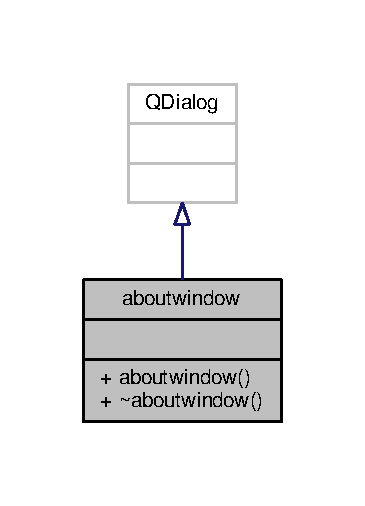
\includegraphics[width=175pt]{classaboutwindow__inherit__graph}
\end{center}
\end{figure}


Collaboration diagram for aboutwindow\+:
\nopagebreak
\begin{figure}[H]
\begin{center}
\leavevmode
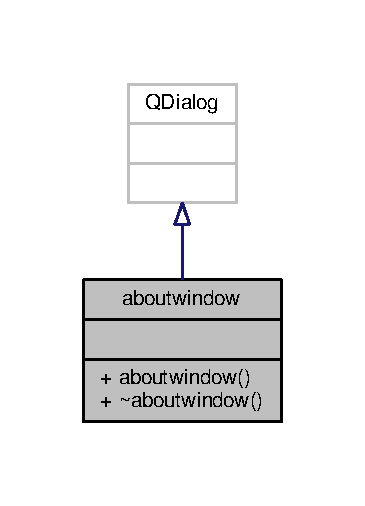
\includegraphics[width=175pt]{classaboutwindow__coll__graph}
\end{center}
\end{figure}
\subsection*{Public Member Functions}
\begin{DoxyCompactItemize}
\item 
\hypertarget{classaboutwindow_a27a819aa0351428d684b12827130f78e}{}{\bfseries aboutwindow} (Q\+Widget $\ast$parent=0)\label{classaboutwindow_a27a819aa0351428d684b12827130f78e}

\end{DoxyCompactItemize}


The documentation for this class was generated from the following files\+:\begin{DoxyCompactItemize}
\item 
source/aboutwindow.\+h\item 
source/aboutwindow.\+cpp\end{DoxyCompactItemize}

\hypertarget{classAdd}{}\section{Add Class Reference}
\label{classAdd}\index{Add@{Add}}


\hyperlink{classAdd}{Add} two doubles G\+P primitive.  




Inheritance diagram for Add\+:
\nopagebreak
\begin{figure}[H]
\begin{center}
\leavevmode
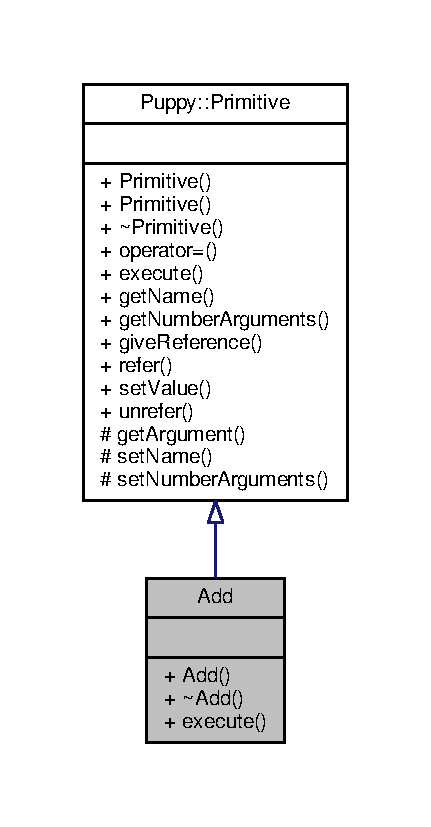
\includegraphics[width=207pt]{classAdd__inherit__graph}
\end{center}
\end{figure}


Collaboration diagram for Add\+:
\nopagebreak
\begin{figure}[H]
\begin{center}
\leavevmode
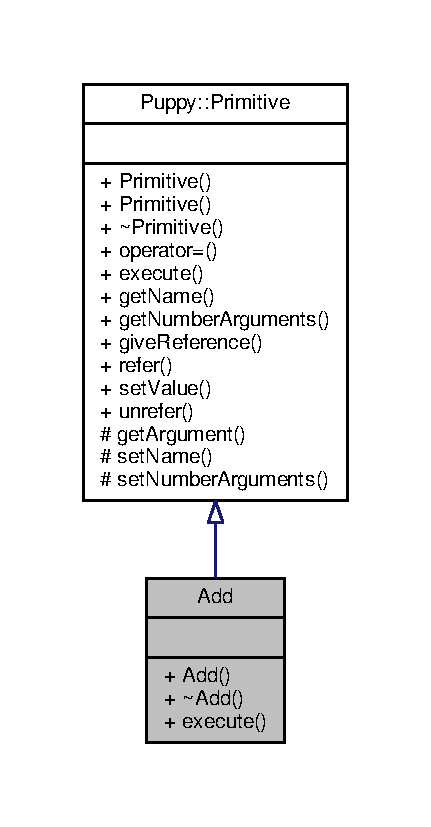
\includegraphics[width=207pt]{classAdd__coll__graph}
\end{center}
\end{figure}
\subsection*{Public Member Functions}
\begin{DoxyCompactItemize}
\item 
\hypertarget{classAdd_a44b62ab4a0b9a4fb3e77427d35e411b9}{}\hyperlink{classAdd_a44b62ab4a0b9a4fb3e77427d35e411b9}{Add} ()\label{classAdd_a44b62ab4a0b9a4fb3e77427d35e411b9}

\begin{DoxyCompactList}\small\item\em Construct \hyperlink{classAdd}{Add} G\+P primitive. \end{DoxyCompactList}\item 
virtual void \hyperlink{classAdd_a5f17154064fd521553352f114db35018}{execute} (void $\ast$out\+Datum, \hyperlink{classPuppy_1_1Context}{Puppy\+::\+Context} \&io\+Context)
\begin{DoxyCompactList}\small\item\em Execute characteristic operation of \hyperlink{classAdd}{Add} primitive. \end{DoxyCompactList}\end{DoxyCompactItemize}
\subsection*{Additional Inherited Members}


\subsection{Detailed Description}
\hyperlink{classAdd}{Add} two doubles G\+P primitive. 

\subsection{Member Function Documentation}
\hypertarget{classAdd_a5f17154064fd521553352f114db35018}{}\index{Add@{Add}!execute@{execute}}
\index{execute@{execute}!Add@{Add}}
\subsubsection[{execute}]{\setlength{\rightskip}{0pt plus 5cm}void Add\+::execute (
\begin{DoxyParamCaption}
\item[{void $\ast$}]{out\+Datum, }
\item[{{\bf Puppy\+::\+Context} \&}]{io\+Context}
\end{DoxyParamCaption}
)\hspace{0.3cm}{\ttfamily [virtual]}}\label{classAdd_a5f17154064fd521553352f114db35018}


Execute characteristic operation of \hyperlink{classAdd}{Add} primitive. 


\begin{DoxyParams}{Parameters}
{\em out\+Datum} & Result of the \hyperlink{classAdd}{Add} operation. \\
\hline
{\em io\+Context} & Evolutionary context. \\
\hline
\end{DoxyParams}


Implements \hyperlink{classPuppy_1_1Primitive_aaef85034e66f49903c591158c3b5ffef}{Puppy\+::\+Primitive}.



The documentation for this class was generated from the following files\+:\begin{DoxyCompactItemize}
\item 
source/puppy\+\_\+regprimitives.\+hpp\item 
source/puppy\+\_\+regprimitives.\+cpp\end{DoxyCompactItemize}

\hypertarget{classPuppy_1_1Context}{}\section{Puppy\+:\+:Context Class Reference}
\label{classPuppy_1_1Context}\index{Puppy\+::\+Context@{Puppy\+::\+Context}}


Evolutionary context.

The evolutionary context includes the execution context used when interpreting the trees along with the problem set-\/up defined with the function and terminal set, and the randomizer.  




Collaboration diagram for Puppy\+:\+:Context\+:
\nopagebreak
\begin{figure}[H]
\begin{center}
\leavevmode
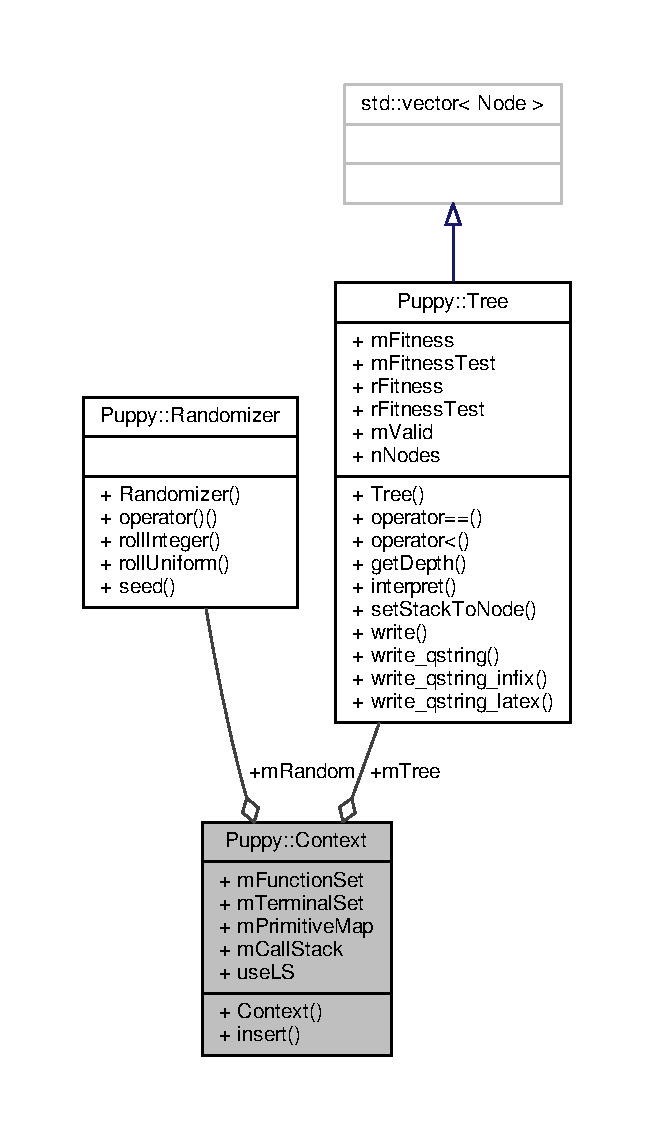
\includegraphics[width=314pt]{classPuppy_1_1Context__coll__graph}
\end{center}
\end{figure}
\subsection*{Public Member Functions}
\begin{DoxyCompactItemize}
\item 
\hypertarget{classPuppy_1_1Context_aac8cb79c11fb01a719665573dbe2401b}{}\hyperlink{classPuppy_1_1Context_aac8cb79c11fb01a719665573dbe2401b}{Context} ()\label{classPuppy_1_1Context_aac8cb79c11fb01a719665573dbe2401b}

\begin{DoxyCompactList}\small\item\em Build an evolutionary context. \end{DoxyCompactList}\item 
void \hyperlink{classPuppy_1_1Context_a8faebd159ee947f837755a6bbc7bccbb}{insert} (\hyperlink{classPuppy_1_1PrimitiveHandle}{Primitive\+Handle} in\+Primitive)
\begin{DoxyCompactList}\small\item\em \hyperlink{classAdd}{Add} a new primitive in the sets of primitive. \end{DoxyCompactList}\end{DoxyCompactItemize}
\subsection*{Public Attributes}
\begin{DoxyCompactItemize}
\item 
\hypertarget{classPuppy_1_1Context_af2256bb8abbf0ba324dfff53a4595dca}{}\hyperlink{classPuppy_1_1Randomizer}{Randomizer} \hyperlink{classPuppy_1_1Context_af2256bb8abbf0ba324dfff53a4595dca}{m\+Random}\label{classPuppy_1_1Context_af2256bb8abbf0ba324dfff53a4595dca}

\begin{DoxyCompactList}\small\item\em Random number generator. \end{DoxyCompactList}\item 
\hypertarget{classPuppy_1_1Context_a3bdbacd226f2ee69b613fc1537c4da92}{}std\+::vector$<$ \hyperlink{classPuppy_1_1PrimitiveHandle}{Primitive\+Handle} $>$ \hyperlink{classPuppy_1_1Context_a3bdbacd226f2ee69b613fc1537c4da92}{m\+Function\+Set}\label{classPuppy_1_1Context_a3bdbacd226f2ee69b613fc1537c4da92}

\begin{DoxyCompactList}\small\item\em Set of functions usable to build trees. \end{DoxyCompactList}\item 
\hypertarget{classPuppy_1_1Context_abd8b7bfb706eb01ccc4e46e78a41385a}{}std\+::vector$<$ \hyperlink{classPuppy_1_1PrimitiveHandle}{Primitive\+Handle} $>$ \hyperlink{classPuppy_1_1Context_abd8b7bfb706eb01ccc4e46e78a41385a}{m\+Terminal\+Set}\label{classPuppy_1_1Context_abd8b7bfb706eb01ccc4e46e78a41385a}

\begin{DoxyCompactList}\small\item\em Set of terminals usable to build trees. \end{DoxyCompactList}\item 
\hypertarget{classPuppy_1_1Context_ac5f0006c4d7f3362ee83d0330c50fa70}{}std\+::map$<$ std\+::string, \hyperlink{classPuppy_1_1PrimitiveHandle}{Primitive\+Handle} $>$ \hyperlink{classPuppy_1_1Context_ac5f0006c4d7f3362ee83d0330c50fa70}{m\+Primitive\+Map}\label{classPuppy_1_1Context_ac5f0006c4d7f3362ee83d0330c50fa70}

\begin{DoxyCompactList}\small\item\em Name-\/primitive map. \end{DoxyCompactList}\item 
\hypertarget{classPuppy_1_1Context_ac26d2fb60125a52a9443c2de815690b2}{}std\+::vector$<$ unsigned int $>$ \hyperlink{classPuppy_1_1Context_ac26d2fb60125a52a9443c2de815690b2}{m\+Call\+Stack}\label{classPuppy_1_1Context_ac26d2fb60125a52a9443c2de815690b2}

\begin{DoxyCompactList}\small\item\em Execution call stack. \end{DoxyCompactList}\item 
\hypertarget{classPuppy_1_1Context_a1e226fd8032307e3fb213bf04cc72b0e}{}\hyperlink{classPuppy_1_1Tree}{Tree} $\ast$ \hyperlink{classPuppy_1_1Context_a1e226fd8032307e3fb213bf04cc72b0e}{m\+Tree}\label{classPuppy_1_1Context_a1e226fd8032307e3fb213bf04cc72b0e}

\begin{DoxyCompactList}\small\item\em Actual tree evaluated. \end{DoxyCompactList}\item 
\hypertarget{classPuppy_1_1Context_abfdb04c41a8a1c6389bd018b44d84fe5}{}bool {\bfseries use\+L\+S}\label{classPuppy_1_1Context_abfdb04c41a8a1c6389bd018b44d84fe5}

\end{DoxyCompactItemize}


\subsection{Detailed Description}
Evolutionary context.

The evolutionary context includes the execution context used when interpreting the trees along with the problem set-\/up defined with the function and terminal set, and the randomizer. 

\subsection{Member Function Documentation}
\hypertarget{classPuppy_1_1Context_a8faebd159ee947f837755a6bbc7bccbb}{}\index{Puppy\+::\+Context@{Puppy\+::\+Context}!insert@{insert}}
\index{insert@{insert}!Puppy\+::\+Context@{Puppy\+::\+Context}}
\subsubsection[{insert}]{\setlength{\rightskip}{0pt plus 5cm}void Puppy\+::\+Context\+::insert (
\begin{DoxyParamCaption}
\item[{{\bf Primitive\+Handle}}]{in\+Primitive}
\end{DoxyParamCaption}
)\hspace{0.3cm}{\ttfamily [inline]}}\label{classPuppy_1_1Context_a8faebd159ee947f837755a6bbc7bccbb}


\hyperlink{classAdd}{Add} a new primitive in the sets of primitive. 


\begin{DoxyParams}{Parameters}
{\em in\+Primitive} & \hyperlink{classPuppy_1_1Primitive}{Primitive} added. \\
\hline
\end{DoxyParams}


The documentation for this class was generated from the following file\+:\begin{DoxyCompactItemize}
\item 
source/puppy\+\_\+context.\+hpp\end{DoxyCompactItemize}

\hypertarget{classCos}{}\section{Cos Class Reference}
\label{classCos}\index{Cos@{Cos}}


Inheritance diagram for Cos\+:
\nopagebreak
\begin{figure}[H]
\begin{center}
\leavevmode
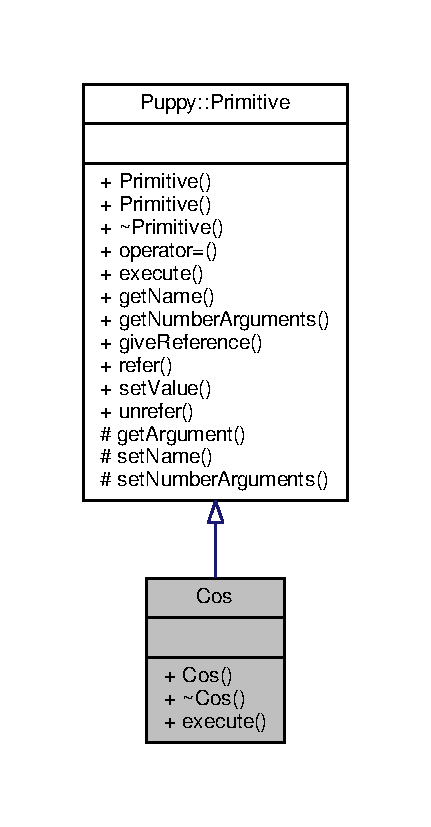
\includegraphics[width=207pt]{classCos__inherit__graph}
\end{center}
\end{figure}


Collaboration diagram for Cos\+:
\nopagebreak
\begin{figure}[H]
\begin{center}
\leavevmode
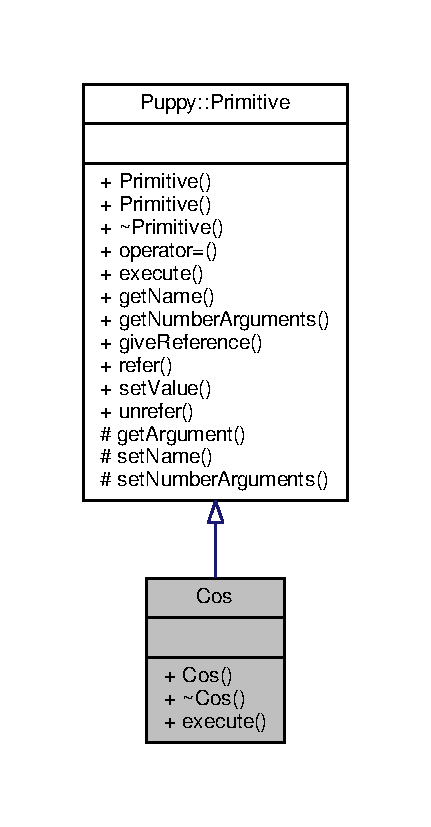
\includegraphics[width=207pt]{classCos__coll__graph}
\end{center}
\end{figure}
\subsection*{Public Member Functions}
\begin{DoxyCompactItemize}
\item 
\hypertarget{classCos_afcabb31f1ff7871afba44a04b78e24c1}{}\hyperlink{classCos_afcabb31f1ff7871afba44a04b78e24c1}{Cos} ()\label{classCos_afcabb31f1ff7871afba44a04b78e24c1}

\begin{DoxyCompactList}\small\item\em Construct \hyperlink{classCos}{Cos} G\+P primitive. \end{DoxyCompactList}\item 
virtual void \hyperlink{classCos_ae797f1f97801e6a64e4bded4f4f4f263}{execute} (void $\ast$out\+Datum, \hyperlink{classPuppy_1_1Context}{Puppy\+::\+Context} \&io\+Context)
\begin{DoxyCompactList}\small\item\em Execute characteristic operation of cos primitive. \end{DoxyCompactList}\end{DoxyCompactItemize}
\subsection*{Additional Inherited Members}


\subsection{Member Function Documentation}
\hypertarget{classCos_ae797f1f97801e6a64e4bded4f4f4f263}{}\index{Cos@{Cos}!execute@{execute}}
\index{execute@{execute}!Cos@{Cos}}
\subsubsection[{execute}]{\setlength{\rightskip}{0pt plus 5cm}void Cos\+::execute (
\begin{DoxyParamCaption}
\item[{void $\ast$}]{out\+Datum, }
\item[{{\bf Puppy\+::\+Context} \&}]{io\+Context}
\end{DoxyParamCaption}
)\hspace{0.3cm}{\ttfamily [virtual]}}\label{classCos_ae797f1f97801e6a64e4bded4f4f4f263}


Execute characteristic operation of cos primitive. 


\begin{DoxyParams}{Parameters}
{\em out\+Datum} & Result of the cos operation. \\
\hline
{\em io\+Context} & Evolutionary context. \\
\hline
\end{DoxyParams}


Implements \hyperlink{classPuppy_1_1Primitive_aaef85034e66f49903c591158c3b5ffef}{Puppy\+::\+Primitive}.



The documentation for this class was generated from the following files\+:\begin{DoxyCompactItemize}
\item 
source/puppy\+\_\+regprimitives.\+hpp\item 
source/puppy\+\_\+regprimitives.\+cpp\end{DoxyCompactItemize}

\hypertarget{classDivide}{}\section{Divide Class Reference}
\label{classDivide}\index{Divide@{Divide}}


Protected division of two doubles G\+P primitive.  




Inheritance diagram for Divide\+:
\nopagebreak
\begin{figure}[H]
\begin{center}
\leavevmode
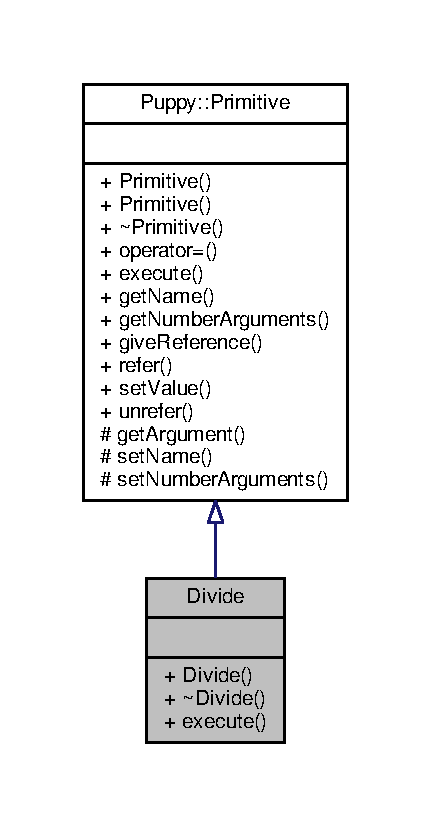
\includegraphics[width=207pt]{classDivide__inherit__graph}
\end{center}
\end{figure}


Collaboration diagram for Divide\+:
\nopagebreak
\begin{figure}[H]
\begin{center}
\leavevmode
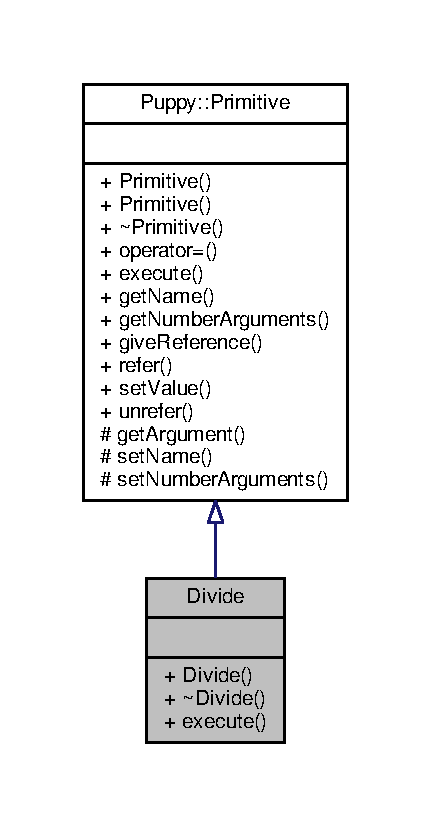
\includegraphics[width=207pt]{classDivide__coll__graph}
\end{center}
\end{figure}
\subsection*{Public Member Functions}
\begin{DoxyCompactItemize}
\item 
\hypertarget{classDivide_ac5f1271d02153b1aa1c7de17c7a09abd}{}\hyperlink{classDivide_ac5f1271d02153b1aa1c7de17c7a09abd}{Divide} ()\label{classDivide_ac5f1271d02153b1aa1c7de17c7a09abd}

\begin{DoxyCompactList}\small\item\em Construct \hyperlink{classDivide}{Divide} G\+P primitive. \end{DoxyCompactList}\item 
virtual void \hyperlink{classDivide_af5ed152cd9a4e65141a59ef78307e87f}{execute} (void $\ast$out\+Datum, \hyperlink{classPuppy_1_1Context}{Puppy\+::\+Context} \&io\+Context)
\begin{DoxyCompactList}\small\item\em Execute characteristic operation of \hyperlink{classDivide}{Divide} primitive. \end{DoxyCompactList}\end{DoxyCompactItemize}
\subsection*{Additional Inherited Members}


\subsection{Detailed Description}
Protected division of two doubles G\+P primitive. 

\subsection{Member Function Documentation}
\hypertarget{classDivide_af5ed152cd9a4e65141a59ef78307e87f}{}\index{Divide@{Divide}!execute@{execute}}
\index{execute@{execute}!Divide@{Divide}}
\subsubsection[{execute}]{\setlength{\rightskip}{0pt plus 5cm}void Divide\+::execute (
\begin{DoxyParamCaption}
\item[{void $\ast$}]{out\+Datum, }
\item[{{\bf Puppy\+::\+Context} \&}]{io\+Context}
\end{DoxyParamCaption}
)\hspace{0.3cm}{\ttfamily [virtual]}}\label{classDivide_af5ed152cd9a4e65141a59ef78307e87f}


Execute characteristic operation of \hyperlink{classDivide}{Divide} primitive. 


\begin{DoxyParams}{Parameters}
{\em out\+Datum} & Result of the \hyperlink{classDivide}{Divide} operation. \\
\hline
{\em io\+Context} & Evolutionary context. \\
\hline
\end{DoxyParams}


Implements \hyperlink{classPuppy_1_1Primitive_aaef85034e66f49903c591158c3b5ffef}{Puppy\+::\+Primitive}.



The documentation for this class was generated from the following files\+:\begin{DoxyCompactItemize}
\item 
source/puppy\+\_\+regprimitives.\+hpp\item 
source/puppy\+\_\+regprimitives.\+cpp\end{DoxyCompactItemize}

\hypertarget{classEdge}{}\section{Edge Class Reference}
\label{classEdge}\index{Edge@{Edge}}


Inheritance diagram for Edge\+:
\nopagebreak
\begin{figure}[H]
\begin{center}
\leavevmode
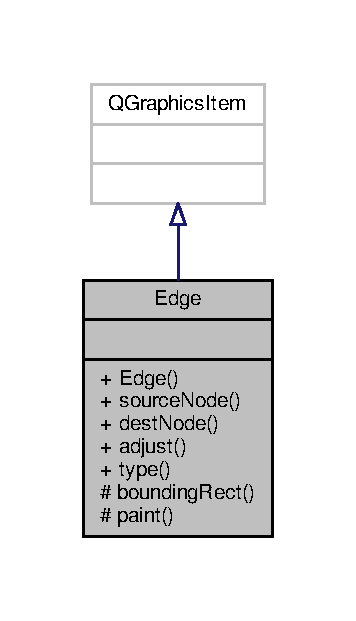
\includegraphics[width=171pt]{classEdge__inherit__graph}
\end{center}
\end{figure}


Collaboration diagram for Edge\+:
\nopagebreak
\begin{figure}[H]
\begin{center}
\leavevmode
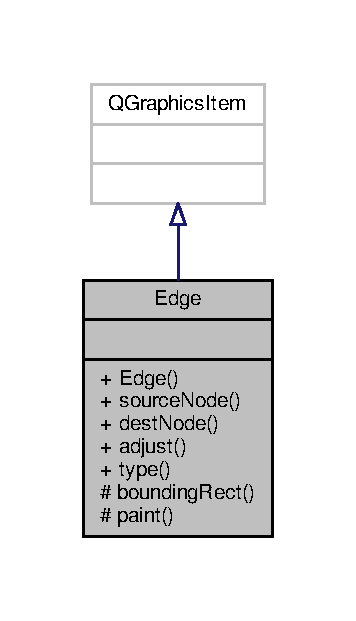
\includegraphics[width=171pt]{classEdge__coll__graph}
\end{center}
\end{figure}
\subsection*{Public Types}
\begin{DoxyCompactItemize}
\item 
\hypertarget{classEdge_a1076c24a9c10f5e019ee362060200329}{}enum \{ {\bfseries Type} = User\+Type + 2
 \}\label{classEdge_a1076c24a9c10f5e019ee362060200329}

\end{DoxyCompactItemize}
\subsection*{Public Member Functions}
\begin{DoxyCompactItemize}
\item 
\hypertarget{classEdge_a2d28ba5ca3502b2134f7d2587e57cae7}{}{\bfseries Edge} (\hyperlink{classNode}{Node} $\ast$source\+Node, \hyperlink{classNode}{Node} $\ast$dest\+Node)\label{classEdge_a2d28ba5ca3502b2134f7d2587e57cae7}

\item 
\hypertarget{classEdge_abd81ba4644f7453ede7f74f442a4c943}{}\hyperlink{classNode}{Node} $\ast$ {\bfseries source\+Node} () const \label{classEdge_abd81ba4644f7453ede7f74f442a4c943}

\item 
\hypertarget{classEdge_a1b844ad6fd91e53003a55ed62d184fac}{}\hyperlink{classNode}{Node} $\ast$ {\bfseries dest\+Node} () const \label{classEdge_a1b844ad6fd91e53003a55ed62d184fac}

\item 
\hypertarget{classEdge_ab554a765fd7a57fcdf289aa51b4df328}{}void {\bfseries adjust} ()\label{classEdge_ab554a765fd7a57fcdf289aa51b4df328}

\item 
\hypertarget{classEdge_ad0859f7b8f96e4ab40edb267743b1c08}{}int {\bfseries type} () const Q\+\_\+\+D\+E\+C\+L\+\_\+\+O\+V\+E\+R\+R\+I\+D\+E\label{classEdge_ad0859f7b8f96e4ab40edb267743b1c08}

\end{DoxyCompactItemize}
\subsection*{Protected Member Functions}
\begin{DoxyCompactItemize}
\item 
\hypertarget{classEdge_a02a869b182dfb09f04be5ee3f0ce56dd}{}Q\+Rect\+F {\bfseries bounding\+Rect} () const Q\+\_\+\+D\+E\+C\+L\+\_\+\+O\+V\+E\+R\+R\+I\+D\+E\label{classEdge_a02a869b182dfb09f04be5ee3f0ce56dd}

\item 
\hypertarget{classEdge_a8e9131800530a799730d2f6dbee21187}{}void {\bfseries paint} (Q\+Painter $\ast$painter, const Q\+Style\+Option\+Graphics\+Item $\ast$option, Q\+Widget $\ast$widget) Q\+\_\+\+D\+E\+C\+L\+\_\+\+O\+V\+E\+R\+R\+I\+D\+E\label{classEdge_a8e9131800530a799730d2f6dbee21187}

\end{DoxyCompactItemize}


The documentation for this class was generated from the following files\+:\begin{DoxyCompactItemize}
\item 
source/edge.\+h\item 
source/edge.\+cpp\end{DoxyCompactItemize}

\hypertarget{classEphemeral}{}\section{Ephemeral Class Reference}
\label{classEphemeral}\index{Ephemeral@{Ephemeral}}


\hyperlink{classEphemeral}{Ephemeral} random constant.  




Inheritance diagram for Ephemeral\+:
\nopagebreak
\begin{figure}[H]
\begin{center}
\leavevmode
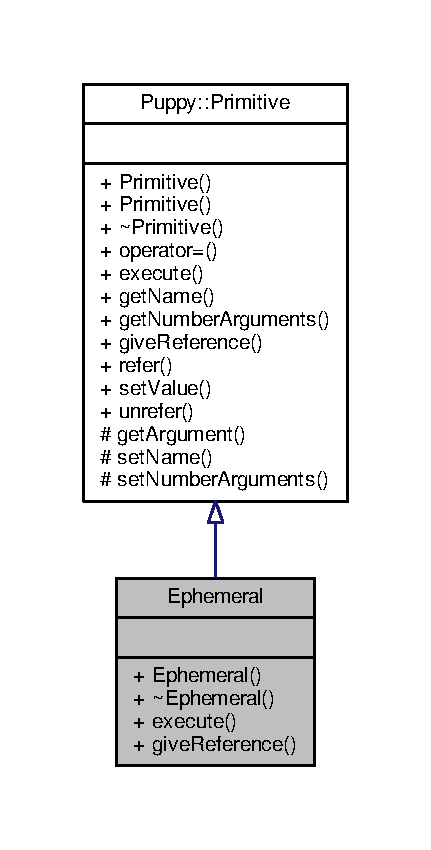
\includegraphics[width=207pt]{classEphemeral__inherit__graph}
\end{center}
\end{figure}


Collaboration diagram for Ephemeral\+:
\nopagebreak
\begin{figure}[H]
\begin{center}
\leavevmode
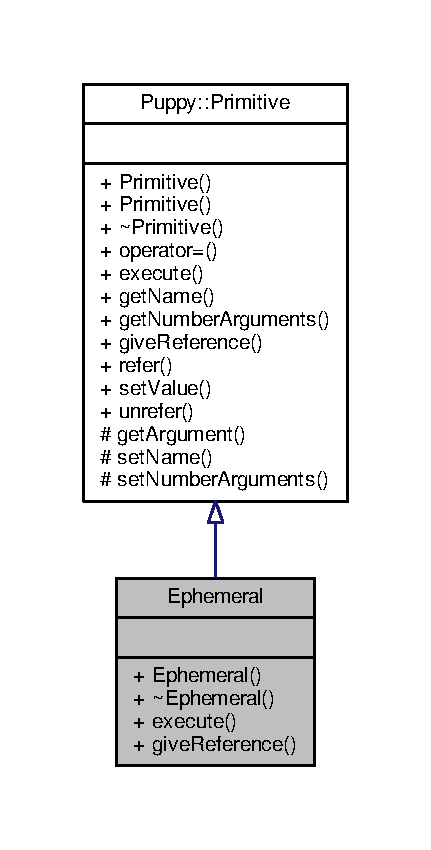
\includegraphics[width=207pt]{classEphemeral__coll__graph}
\end{center}
\end{figure}
\subsection*{Public Member Functions}
\begin{DoxyCompactItemize}
\item 
\hypertarget{classEphemeral_ac6c554dd7fc112356dc1794d5579f28e}{}\hyperlink{classEphemeral_ac6c554dd7fc112356dc1794d5579f28e}{Ephemeral} ()\label{classEphemeral_ac6c554dd7fc112356dc1794d5579f28e}

\begin{DoxyCompactList}\small\item\em Construct ephemeral random constant generator primitive. \end{DoxyCompactList}\item 
virtual void \hyperlink{classEphemeral_a69fb1365baddf81c9f1cd7c35a6bad16}{execute} (void $\ast$out\+Datum, \hyperlink{classPuppy_1_1Context}{Puppy\+::\+Context} \&io\+Context)
\begin{DoxyCompactList}\small\item\em Dummy function, ephemeral primitive is used only to generate constants. \end{DoxyCompactList}\item 
virtual \hyperlink{classPuppy_1_1PrimitiveHandle}{Puppy\+::\+Primitive\+Handle} \hyperlink{classEphemeral_a4c8bf775486a868d9011c4b9d93e7547}{give\+Reference} (\hyperlink{classPuppy_1_1Context}{Puppy\+::\+Context} \&io\+Context)
\begin{DoxyCompactList}\small\item\em Generate random constant and return as primitive handle. \end{DoxyCompactList}\end{DoxyCompactItemize}
\subsection*{Additional Inherited Members}


\subsection{Detailed Description}
\hyperlink{classEphemeral}{Ephemeral} random constant. 

\subsection{Member Function Documentation}
\hypertarget{classEphemeral_a69fb1365baddf81c9f1cd7c35a6bad16}{}\index{Ephemeral@{Ephemeral}!execute@{execute}}
\index{execute@{execute}!Ephemeral@{Ephemeral}}
\subsubsection[{execute}]{\setlength{\rightskip}{0pt plus 5cm}void Ephemeral\+::execute (
\begin{DoxyParamCaption}
\item[{void $\ast$}]{out\+Datum, }
\item[{{\bf Puppy\+::\+Context} \&}]{io\+Context}
\end{DoxyParamCaption}
)\hspace{0.3cm}{\ttfamily [virtual]}}\label{classEphemeral_a69fb1365baddf81c9f1cd7c35a6bad16}


Dummy function, ephemeral primitive is used only to generate constants. 


\begin{DoxyParams}{Parameters}
{\em out\+Datum} & Result of the \hyperlink{classDivide}{Divide} operation. \\
\hline
{\em io\+Context} & Evolutionary context. \\
\hline
\end{DoxyParams}


Implements \hyperlink{classPuppy_1_1Primitive_aaef85034e66f49903c591158c3b5ffef}{Puppy\+::\+Primitive}.

\hypertarget{classEphemeral_a4c8bf775486a868d9011c4b9d93e7547}{}\index{Ephemeral@{Ephemeral}!give\+Reference@{give\+Reference}}
\index{give\+Reference@{give\+Reference}!Ephemeral@{Ephemeral}}
\subsubsection[{give\+Reference}]{\setlength{\rightskip}{0pt plus 5cm}{\bf Primitive\+Handle} Ephemeral\+::give\+Reference (
\begin{DoxyParamCaption}
\item[{{\bf Puppy\+::\+Context} \&}]{io\+Context}
\end{DoxyParamCaption}
)\hspace{0.3cm}{\ttfamily [virtual]}}\label{classEphemeral_a4c8bf775486a868d9011c4b9d93e7547}


Generate random constant and return as primitive handle. 


\begin{DoxyParams}{Parameters}
{\em io\+Context} & Evolutionary context. \\
\hline
\end{DoxyParams}


Reimplemented from \hyperlink{classPuppy_1_1Primitive_a0319f5a18dd42fe96c77c895948acc2a}{Puppy\+::\+Primitive}.



The documentation for this class was generated from the following files\+:\begin{DoxyCompactItemize}
\item 
source/puppy\+\_\+regprimitives.\+hpp\item 
source/puppy\+\_\+regprimitives.\+cpp\end{DoxyCompactItemize}

\hypertarget{classExp}{}\section{Exp Class Reference}
\label{classExp}\index{Exp@{Exp}}


Inheritance diagram for Exp\+:
\nopagebreak
\begin{figure}[H]
\begin{center}
\leavevmode
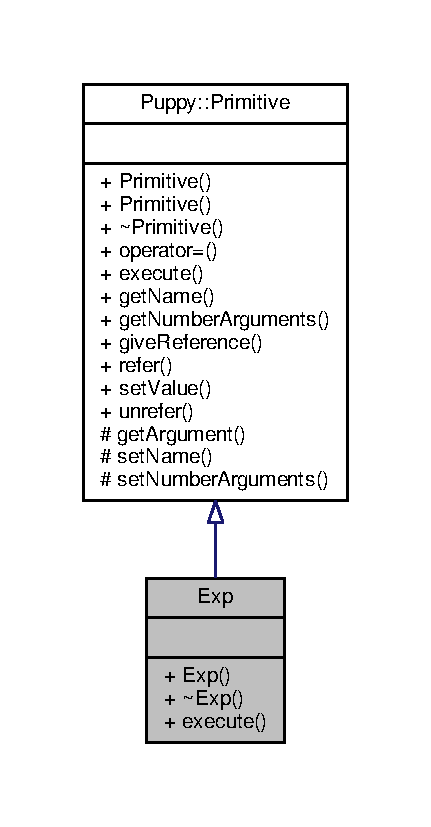
\includegraphics[width=207pt]{classExp__inherit__graph}
\end{center}
\end{figure}


Collaboration diagram for Exp\+:
\nopagebreak
\begin{figure}[H]
\begin{center}
\leavevmode
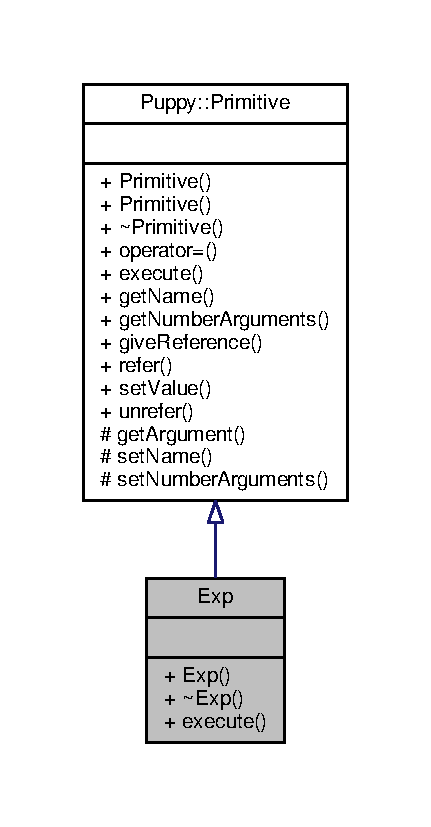
\includegraphics[width=207pt]{classExp__coll__graph}
\end{center}
\end{figure}
\subsection*{Public Member Functions}
\begin{DoxyCompactItemize}
\item 
\hypertarget{classExp_aacde419dcd80d7576643b4b529c0168f}{}\hyperlink{classExp_aacde419dcd80d7576643b4b529c0168f}{Exp} ()\label{classExp_aacde419dcd80d7576643b4b529c0168f}

\begin{DoxyCompactList}\small\item\em Construct \hyperlink{classExp}{Exp} G\+P primitive. \end{DoxyCompactList}\item 
virtual void \hyperlink{classExp_af04e8771ab5a8b572779d0703efa2736}{execute} (void $\ast$out\+Datum, \hyperlink{classPuppy_1_1Context}{Puppy\+::\+Context} \&io\+Context)
\begin{DoxyCompactList}\small\item\em Execute characteristic operation of exp primitive. \end{DoxyCompactList}\end{DoxyCompactItemize}
\subsection*{Additional Inherited Members}


\subsection{Member Function Documentation}
\hypertarget{classExp_af04e8771ab5a8b572779d0703efa2736}{}\index{Exp@{Exp}!execute@{execute}}
\index{execute@{execute}!Exp@{Exp}}
\subsubsection[{execute}]{\setlength{\rightskip}{0pt plus 5cm}void Exp\+::execute (
\begin{DoxyParamCaption}
\item[{void $\ast$}]{out\+Datum, }
\item[{{\bf Puppy\+::\+Context} \&}]{io\+Context}
\end{DoxyParamCaption}
)\hspace{0.3cm}{\ttfamily [virtual]}}\label{classExp_af04e8771ab5a8b572779d0703efa2736}


Execute characteristic operation of exp primitive. 


\begin{DoxyParams}{Parameters}
{\em out\+Datum} & Result of the exp operation. \\
\hline
{\em io\+Context} & Evolutionary context. \\
\hline
\end{DoxyParams}


Implements \hyperlink{classPuppy_1_1Primitive_aaef85034e66f49903c591158c3b5ffef}{Puppy\+::\+Primitive}.



The documentation for this class was generated from the following files\+:\begin{DoxyCompactItemize}
\item 
source/puppy\+\_\+regprimitives.\+hpp\item 
source/puppy\+\_\+regprimitives.\+cpp\end{DoxyCompactItemize}

\hypertarget{structWorker_1_1fitnessdata}{}\section{Worker\+:\+:fitnessdata Struct Reference}
\label{structWorker_1_1fitnessdata}\index{Worker\+::fitnessdata@{Worker\+::fitnessdata}}


Collaboration diagram for Worker\+:\+:fitnessdata\+:
\nopagebreak
\begin{figure}[H]
\begin{center}
\leavevmode
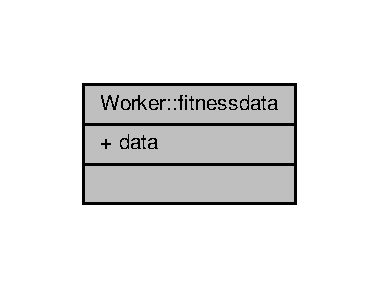
\includegraphics[width=182pt]{structWorker_1_1fitnessdata__coll__graph}
\end{center}
\end{figure}
\subsection*{Public Attributes}
\begin{DoxyCompactItemize}
\item 
\hypertarget{structWorker_1_1fitnessdata_a3baa133e61e81814d5000a4018a3bc92}{}double $\ast$$\ast$ {\bfseries data}\label{structWorker_1_1fitnessdata_a3baa133e61e81814d5000a4018a3bc92}

\end{DoxyCompactItemize}


The documentation for this struct was generated from the following file\+:\begin{DoxyCompactItemize}
\item 
source/worker.\+h\end{DoxyCompactItemize}

\hypertarget{classLog}{}\section{Log Class Reference}
\label{classLog}\index{Log@{Log}}


Inheritance diagram for Log\+:
\nopagebreak
\begin{figure}[H]
\begin{center}
\leavevmode
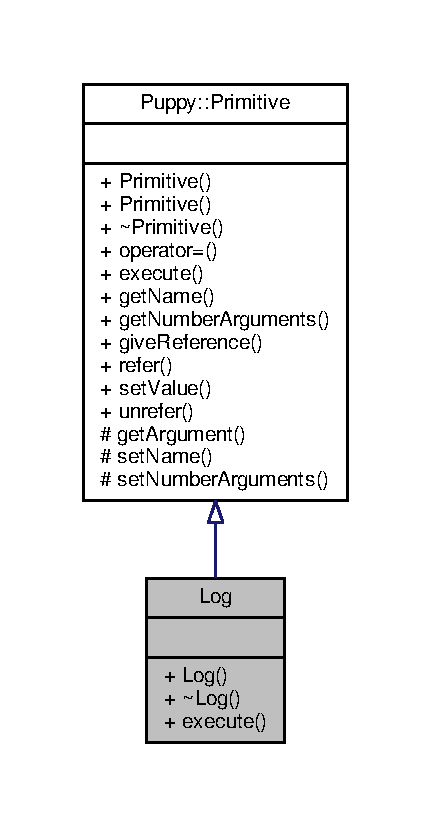
\includegraphics[width=207pt]{classLog__inherit__graph}
\end{center}
\end{figure}


Collaboration diagram for Log\+:
\nopagebreak
\begin{figure}[H]
\begin{center}
\leavevmode
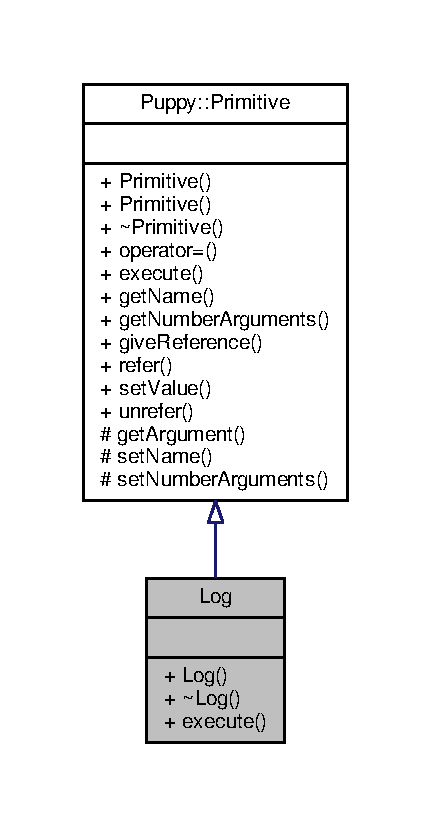
\includegraphics[width=207pt]{classLog__coll__graph}
\end{center}
\end{figure}
\subsection*{Public Member Functions}
\begin{DoxyCompactItemize}
\item 
\hypertarget{classLog_af6071a60aa52b6c1b511f99b4bc1b8fe}{}\hyperlink{classLog_af6071a60aa52b6c1b511f99b4bc1b8fe}{Log} ()\label{classLog_af6071a60aa52b6c1b511f99b4bc1b8fe}

\begin{DoxyCompactList}\small\item\em Construct \hyperlink{classLog}{Log} G\+P primitive. \end{DoxyCompactList}\item 
virtual void \hyperlink{classLog_a0f034cdf9ef168f4ee556e24934519ab}{execute} (void $\ast$out\+Datum, \hyperlink{classPuppy_1_1Context}{Puppy\+::\+Context} \&io\+Context)
\begin{DoxyCompactList}\small\item\em Execute characteristic operation of log primitive. \end{DoxyCompactList}\end{DoxyCompactItemize}
\subsection*{Additional Inherited Members}


\subsection{Member Function Documentation}
\hypertarget{classLog_a0f034cdf9ef168f4ee556e24934519ab}{}\index{Log@{Log}!execute@{execute}}
\index{execute@{execute}!Log@{Log}}
\subsubsection[{execute}]{\setlength{\rightskip}{0pt plus 5cm}void Log\+::execute (
\begin{DoxyParamCaption}
\item[{void $\ast$}]{out\+Datum, }
\item[{{\bf Puppy\+::\+Context} \&}]{io\+Context}
\end{DoxyParamCaption}
)\hspace{0.3cm}{\ttfamily [virtual]}}\label{classLog_a0f034cdf9ef168f4ee556e24934519ab}


Execute characteristic operation of log primitive. 


\begin{DoxyParams}{Parameters}
{\em out\+Datum} & Result of the log operation. \\
\hline
{\em io\+Context} & Evolutionary context. \\
\hline
\end{DoxyParams}


Implements \hyperlink{classPuppy_1_1Primitive_aaef85034e66f49903c591158c3b5ffef}{Puppy\+::\+Primitive}.



The documentation for this class was generated from the following files\+:\begin{DoxyCompactItemize}
\item 
source/puppy\+\_\+regprimitives.\+hpp\item 
source/puppy\+\_\+regprimitives.\+cpp\end{DoxyCompactItemize}

\hypertarget{classMainWindow}{}\section{Main\+Window Class Reference}
\label{classMainWindow}\index{Main\+Window@{Main\+Window}}


Inheritance diagram for Main\+Window\+:
\nopagebreak
\begin{figure}[H]
\begin{center}
\leavevmode
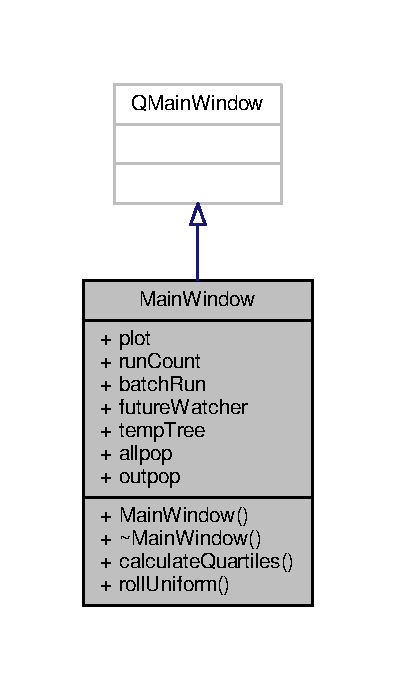
\includegraphics[width=190pt]{classMainWindow__inherit__graph}
\end{center}
\end{figure}


Collaboration diagram for Main\+Window\+:
\nopagebreak
\begin{figure}[H]
\begin{center}
\leavevmode
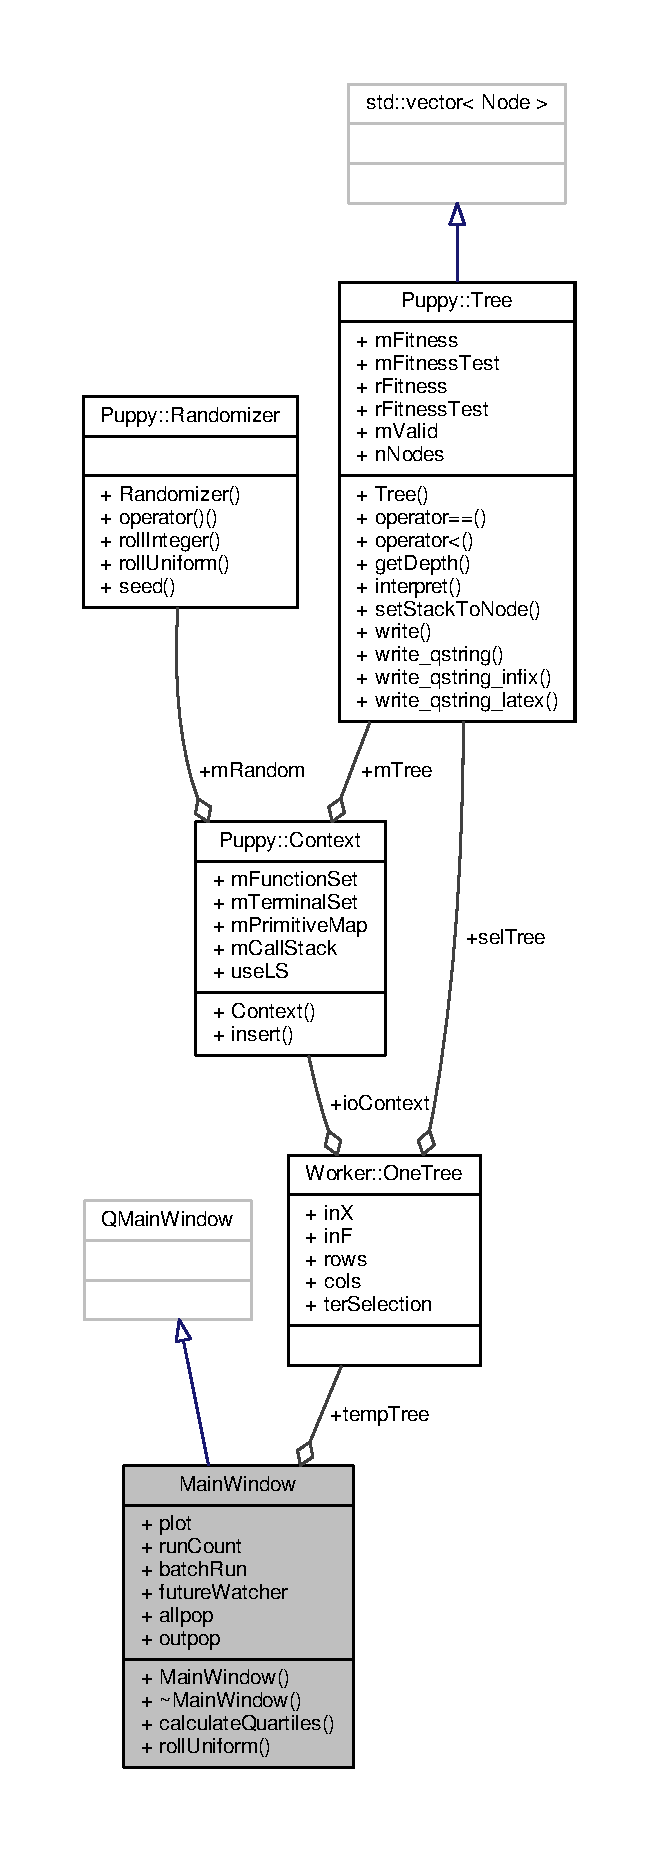
\includegraphics[height=550pt]{classMainWindow__coll__graph}
\end{center}
\end{figure}
\subsection*{Signals}
\begin{DoxyCompactItemize}
\item 
\hypertarget{classMainWindow_a96209ee66905f9c12819a54ec55e9355}{}void {\bfseries finished\+Calc} ()\label{classMainWindow_a96209ee66905f9c12819a54ec55e9355}

\end{DoxyCompactItemize}
\subsection*{Public Member Functions}
\begin{DoxyCompactItemize}
\item 
\hypertarget{classMainWindow_a8b244be8b7b7db1b08de2a2acb9409db}{}{\bfseries Main\+Window} (Q\+Widget $\ast$parent=0)\label{classMainWindow_a8b244be8b7b7db1b08de2a2acb9409db}

\item 
\hypertarget{classMainWindow_ac686d9af408fec710cd42955c43c845c}{}void {\bfseries calculate\+Quartiles} (std\+::vector$<$ double $>$ data, double \&Q1, double \&Q2, double \&Q3, double \&min, double \&max, Q\+Vector$<$ double $>$ \&outliers)\label{classMainWindow_ac686d9af408fec710cd42955c43c845c}

\item 
\hypertarget{classMainWindow_a7a4f624daccfc6abe3868b0ba93a03b2}{}double {\bfseries roll\+Uniform} (double in\+Low, double in\+Up)\label{classMainWindow_a7a4f624daccfc6abe3868b0ba93a03b2}

\end{DoxyCompactItemize}
\subsection*{Public Attributes}
\begin{DoxyCompactItemize}
\item 
\hypertarget{classMainWindow_a8a5d5f218964eaa481e774b56d99b257}{}Qwt3\+D\+::\+Grid\+Plot $\ast$ {\bfseries plot}\label{classMainWindow_a8a5d5f218964eaa481e774b56d99b257}

\item 
\hypertarget{classMainWindow_a576eb30972250aad507588f806458ae3}{}int {\bfseries run\+Count}\label{classMainWindow_a576eb30972250aad507588f806458ae3}

\item 
\hypertarget{classMainWindow_a88110b77c2e35f2264b5cac62f59947e}{}int {\bfseries batch\+Run}\label{classMainWindow_a88110b77c2e35f2264b5cac62f59947e}

\item 
\hypertarget{classMainWindow_aca92ba16d73ac4d621564d6a894aaf6a}{}Q\+Future\+Watcher$<$ Q\+Vector$<$ \hyperlink{classPuppy_1_1Tree}{Puppy\+::\+Tree} $>$ $>$ {\bfseries future\+Watcher}\label{classMainWindow_aca92ba16d73ac4d621564d6a894aaf6a}

\item 
\hypertarget{classMainWindow_a8afe9c18906c2375f2680cc0db63bb87}{}\hyperlink{structWorker_1_1OneTree}{Worker\+::\+One\+Tree} {\bfseries temp\+Tree}\label{classMainWindow_a8afe9c18906c2375f2680cc0db63bb87}

\item 
\hypertarget{classMainWindow_a1f255e88b4b9f1fff19b78ffabac5186}{}Q\+Vector$<$ \hyperlink{structWorker_1_1OneTree}{Worker\+::\+One\+Tree} $>$ {\bfseries allpop}\label{classMainWindow_a1f255e88b4b9f1fff19b78ffabac5186}

\item 
\hypertarget{classMainWindow_a45e011664a91877766b8ddd3359509a7}{}Q\+Vector$<$ \hyperlink{classPuppy_1_1Tree}{Puppy\+::\+Tree} $>$ {\bfseries outpop}\label{classMainWindow_a45e011664a91877766b8ddd3359509a7}

\end{DoxyCompactItemize}


The documentation for this class was generated from the following files\+:\begin{DoxyCompactItemize}
\item 
source/mainwindow.\+h\item 
source/benchmark.\+cpp\item 
source/mainwindow.\+cpp\end{DoxyCompactItemize}

\hypertarget{classMatrix}{}\section{Matrix Class Reference}
\label{classMatrix}\index{Matrix@{Matrix}}


Collaboration diagram for Matrix\+:
\nopagebreak
\begin{figure}[H]
\begin{center}
\leavevmode
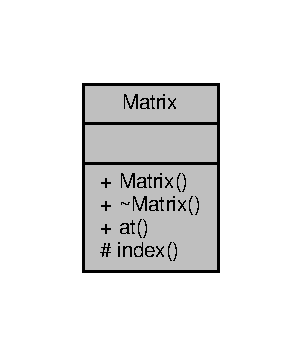
\includegraphics[width=145pt]{classMatrix__coll__graph}
\end{center}
\end{figure}
\subsection*{Public Member Functions}
\begin{DoxyCompactItemize}
\item 
\hypertarget{classMatrix_ae940d9b978841f5f497b7b7f81c63d23}{}{\bfseries Matrix} (int w, int h)\label{classMatrix_ae940d9b978841f5f497b7b7f81c63d23}

\item 
\hypertarget{classMatrix_a99fbc0ee3fe5a4cc6ba9b8b91244387a}{}int {\bfseries at} (int x, int y) const \label{classMatrix_a99fbc0ee3fe5a4cc6ba9b8b91244387a}

\end{DoxyCompactItemize}
\subsection*{Protected Member Functions}
\begin{DoxyCompactItemize}
\item 
\hypertarget{classMatrix_a29ad13a5d17d7be2b7c0cdcb93b600fe}{}int {\bfseries index} (int x, int y) const \label{classMatrix_a29ad13a5d17d7be2b7c0cdcb93b600fe}

\end{DoxyCompactItemize}


The documentation for this class was generated from the following file\+:\begin{DoxyCompactItemize}
\item 
source/matrix.\+h\end{DoxyCompactItemize}

\hypertarget{classMultiply}{}\section{Multiply Class Reference}
\label{classMultiply}\index{Multiply@{Multiply}}


\hyperlink{classMultiply}{Multiply} two doubles G\+P primitive.  




Inheritance diagram for Multiply\+:
\nopagebreak
\begin{figure}[H]
\begin{center}
\leavevmode
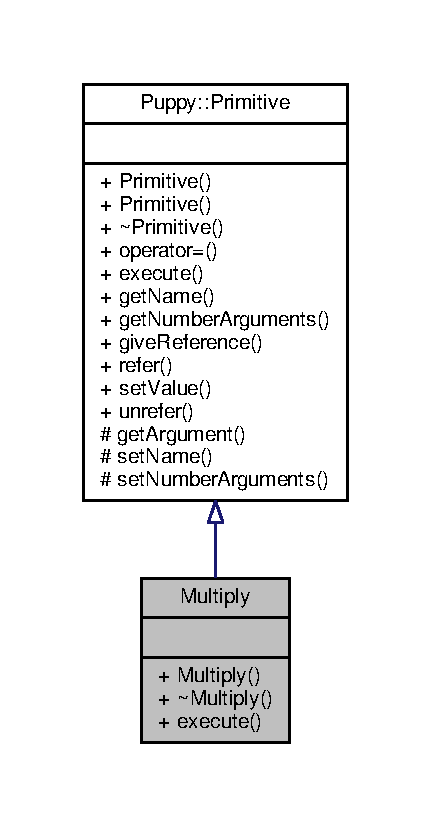
\includegraphics[width=207pt]{classMultiply__inherit__graph}
\end{center}
\end{figure}


Collaboration diagram for Multiply\+:
\nopagebreak
\begin{figure}[H]
\begin{center}
\leavevmode
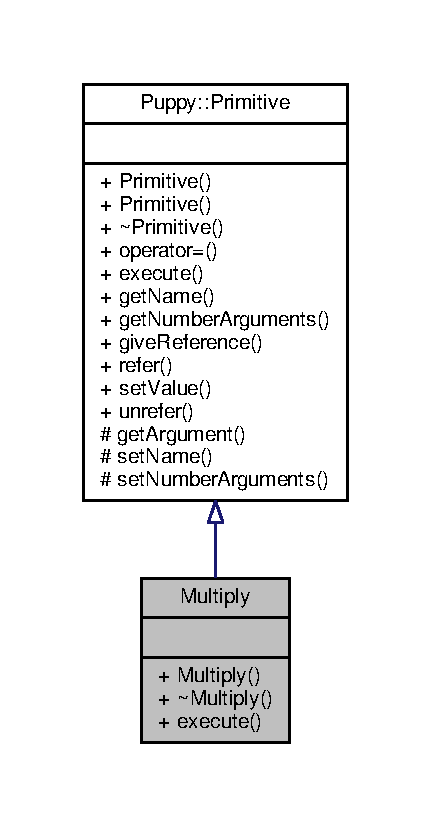
\includegraphics[width=207pt]{classMultiply__coll__graph}
\end{center}
\end{figure}
\subsection*{Public Member Functions}
\begin{DoxyCompactItemize}
\item 
\hypertarget{classMultiply_ae7af092a55a333b67bd20ffa86d6cb9e}{}\hyperlink{classMultiply_ae7af092a55a333b67bd20ffa86d6cb9e}{Multiply} ()\label{classMultiply_ae7af092a55a333b67bd20ffa86d6cb9e}

\begin{DoxyCompactList}\small\item\em Construct \hyperlink{classMultiply}{Multiply} G\+P primitive. \end{DoxyCompactList}\item 
virtual void \hyperlink{classMultiply_a965412103b5dadd21ed4d58c8d6c6d87}{execute} (void $\ast$out\+Datum, \hyperlink{classPuppy_1_1Context}{Puppy\+::\+Context} \&io\+Context)
\begin{DoxyCompactList}\small\item\em Execute characteristic operation of \hyperlink{classMultiply}{Multiply} primitive. \end{DoxyCompactList}\end{DoxyCompactItemize}
\subsection*{Additional Inherited Members}


\subsection{Detailed Description}
\hyperlink{classMultiply}{Multiply} two doubles G\+P primitive. 

\subsection{Member Function Documentation}
\hypertarget{classMultiply_a965412103b5dadd21ed4d58c8d6c6d87}{}\index{Multiply@{Multiply}!execute@{execute}}
\index{execute@{execute}!Multiply@{Multiply}}
\subsubsection[{execute}]{\setlength{\rightskip}{0pt plus 5cm}void Multiply\+::execute (
\begin{DoxyParamCaption}
\item[{void $\ast$}]{out\+Datum, }
\item[{{\bf Puppy\+::\+Context} \&}]{io\+Context}
\end{DoxyParamCaption}
)\hspace{0.3cm}{\ttfamily [virtual]}}\label{classMultiply_a965412103b5dadd21ed4d58c8d6c6d87}


Execute characteristic operation of \hyperlink{classMultiply}{Multiply} primitive. 


\begin{DoxyParams}{Parameters}
{\em out\+Datum} & Result of the \hyperlink{classMultiply}{Multiply} operation. \\
\hline
{\em io\+Context} & Evolutionary context. \\
\hline
\end{DoxyParams}


Implements \hyperlink{classPuppy_1_1Primitive_aaef85034e66f49903c591158c3b5ffef}{Puppy\+::\+Primitive}.



The documentation for this class was generated from the following files\+:\begin{DoxyCompactItemize}
\item 
source/puppy\+\_\+regprimitives.\+hpp\item 
source/puppy\+\_\+regprimitives.\+cpp\end{DoxyCompactItemize}

\hypertarget{structPuppy_1_1Node}{}\section{Puppy\+:\+:Node Struct Reference}
\label{structPuppy_1_1Node}\index{Puppy\+::\+Node@{Puppy\+::\+Node}}


G\+P tree node structure.  




Collaboration diagram for Puppy\+:\+:Node\+:
\nopagebreak
\begin{figure}[H]
\begin{center}
\leavevmode
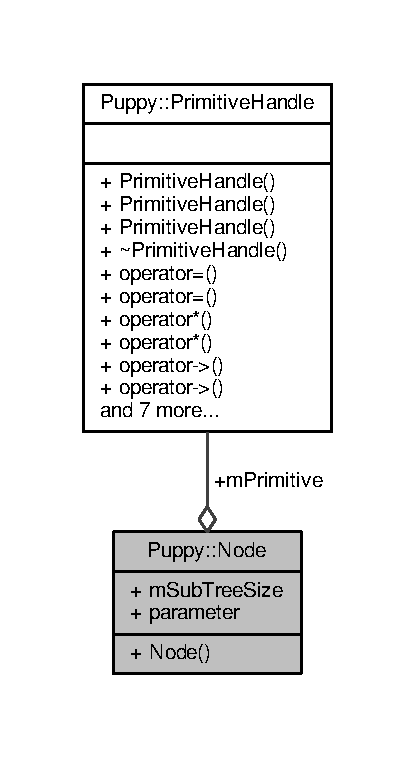
\includegraphics[width=199pt]{structPuppy_1_1Node__coll__graph}
\end{center}
\end{figure}
\subsection*{Public Member Functions}
\begin{DoxyCompactItemize}
\item 
\hyperlink{structPuppy_1_1Node_a766ad2009752aa91f8c5a66753c9d1d7}{Node} (\hyperlink{classPuppy_1_1PrimitiveHandle}{Primitive\+Handle} in\+Primitive=N\+U\+L\+L, unsigned int in\+Sub\+Tree\+Size=0, float in\+Parameter=1)
\begin{DoxyCompactList}\small\item\em Construct a tree node. \end{DoxyCompactList}\end{DoxyCompactItemize}
\subsection*{Public Attributes}
\begin{DoxyCompactItemize}
\item 
\hypertarget{structPuppy_1_1Node_a7be72339910bf7e5333f8a03286c5ec7}{}\hyperlink{classPuppy_1_1PrimitiveHandle}{Primitive\+Handle} \hyperlink{structPuppy_1_1Node_a7be72339910bf7e5333f8a03286c5ec7}{m\+Primitive}\label{structPuppy_1_1Node_a7be72339910bf7e5333f8a03286c5ec7}

\begin{DoxyCompactList}\small\item\em Smart pointer to the associated primitive. \end{DoxyCompactList}\item 
\hypertarget{structPuppy_1_1Node_a047647abeb212563a74933d85306ace0}{}unsigned int \hyperlink{structPuppy_1_1Node_a047647abeb212563a74933d85306ace0}{m\+Sub\+Tree\+Size}\label{structPuppy_1_1Node_a047647abeb212563a74933d85306ace0}

\begin{DoxyCompactList}\small\item\em Sub-\/tree size, including actual node. \end{DoxyCompactList}\item 
\hypertarget{structPuppy_1_1Node_a2bacb0c85f6144192d61dd3af48e7a46}{}float \hyperlink{structPuppy_1_1Node_a2bacb0c85f6144192d61dd3af48e7a46}{parameter}\label{structPuppy_1_1Node_a2bacb0c85f6144192d61dd3af48e7a46}

\begin{DoxyCompactList}\small\item\em Parameter associated with node. \end{DoxyCompactList}\end{DoxyCompactItemize}


\subsection{Detailed Description}
G\+P tree node structure. 

\subsection{Constructor \& Destructor Documentation}
\hypertarget{structPuppy_1_1Node_a766ad2009752aa91f8c5a66753c9d1d7}{}\index{Puppy\+::\+Node@{Puppy\+::\+Node}!Node@{Node}}
\index{Node@{Node}!Puppy\+::\+Node@{Puppy\+::\+Node}}
\subsubsection[{Node}]{\setlength{\rightskip}{0pt plus 5cm}Puppy\+::\+Node\+::\+Node (
\begin{DoxyParamCaption}
\item[{{\bf Primitive\+Handle}}]{in\+Primitive = {\ttfamily NULL}, }
\item[{unsigned int}]{in\+Sub\+Tree\+Size = {\ttfamily 0}, }
\item[{float}]{in\+Parameter = {\ttfamily 1}}
\end{DoxyParamCaption}
)\hspace{0.3cm}{\ttfamily [inline]}, {\ttfamily [explicit]}}\label{structPuppy_1_1Node_a766ad2009752aa91f8c5a66753c9d1d7}


Construct a tree node. 


\begin{DoxyParams}{Parameters}
{\em in\+Primitive} & Reference to the associated primitive. \\
\hline
{\em in\+Sub\+Tree\+Size} & Sub-\/tree size value. \\
\hline
\end{DoxyParams}


The documentation for this struct was generated from the following file\+:\begin{DoxyCompactItemize}
\item 
source/puppy\+\_\+tree.\+hpp\end{DoxyCompactItemize}

\hypertarget{classNode}{}\section{Node Class Reference}
\label{classNode}\index{Node@{Node}}


Inheritance diagram for Node\+:
\nopagebreak
\begin{figure}[H]
\begin{center}
\leavevmode
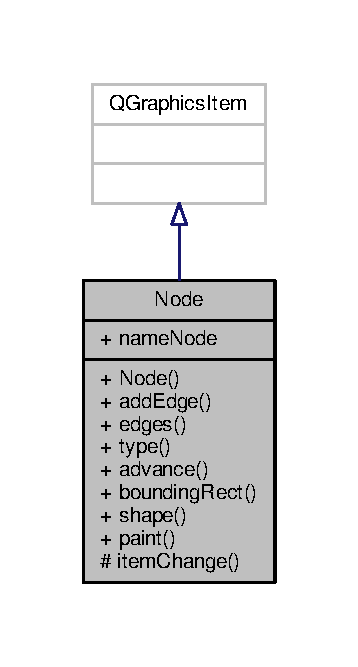
\includegraphics[width=172pt]{classNode__inherit__graph}
\end{center}
\end{figure}


Collaboration diagram for Node\+:
\nopagebreak
\begin{figure}[H]
\begin{center}
\leavevmode
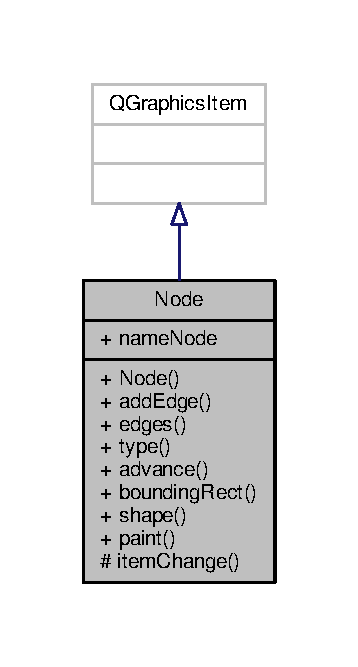
\includegraphics[width=172pt]{classNode__coll__graph}
\end{center}
\end{figure}
\subsection*{Public Types}
\begin{DoxyCompactItemize}
\item 
\hypertarget{classNode_ae716c5198bdf4b0a810324756b0f8f11}{}enum \{ {\bfseries Type} = User\+Type + 1
 \}\label{classNode_ae716c5198bdf4b0a810324756b0f8f11}

\end{DoxyCompactItemize}
\subsection*{Public Member Functions}
\begin{DoxyCompactItemize}
\item 
\hypertarget{classNode_a1090d2bb7bd9193be765a03984b7b101}{}{\bfseries Node} (Graph\+Widget $\ast$graph\+Widget)\label{classNode_a1090d2bb7bd9193be765a03984b7b101}

\item 
\hypertarget{classNode_af761aaef36a761a90c4f148a6add914d}{}void {\bfseries add\+Edge} (\hyperlink{classEdge}{Edge} $\ast$edge)\label{classNode_af761aaef36a761a90c4f148a6add914d}

\item 
\hypertarget{classNode_a339261597715c88141ccb52d8e10f38c}{}Q\+List$<$ \hyperlink{classEdge}{Edge} $\ast$ $>$ {\bfseries edges} () const \label{classNode_a339261597715c88141ccb52d8e10f38c}

\item 
\hypertarget{classNode_a5ff23cc2756595673d0379f19b9a0de9}{}int {\bfseries type} () const Q\+\_\+\+D\+E\+C\+L\+\_\+\+O\+V\+E\+R\+R\+I\+D\+E\label{classNode_a5ff23cc2756595673d0379f19b9a0de9}

\item 
\hypertarget{classNode_ad034abb95cd42d4e577aeb5009ae8d23}{}bool {\bfseries advance} ()\label{classNode_ad034abb95cd42d4e577aeb5009ae8d23}

\item 
\hypertarget{classNode_a91b9aa621ce72fd974ab972ffeb6ec52}{}Q\+Rect\+F {\bfseries bounding\+Rect} () const Q\+\_\+\+D\+E\+C\+L\+\_\+\+O\+V\+E\+R\+R\+I\+D\+E\label{classNode_a91b9aa621ce72fd974ab972ffeb6ec52}

\item 
\hypertarget{classNode_aa1a523740f6a0694abbe690e07eb1d36}{}Q\+Painter\+Path {\bfseries shape} () const Q\+\_\+\+D\+E\+C\+L\+\_\+\+O\+V\+E\+R\+R\+I\+D\+E\label{classNode_aa1a523740f6a0694abbe690e07eb1d36}

\item 
\hypertarget{classNode_afa10e3bbea7f308c3eddcc6097748d13}{}void {\bfseries paint} (Q\+Painter $\ast$painter, const Q\+Style\+Option\+Graphics\+Item $\ast$option, Q\+Widget $\ast$widget) Q\+\_\+\+D\+E\+C\+L\+\_\+\+O\+V\+E\+R\+R\+I\+D\+E\label{classNode_afa10e3bbea7f308c3eddcc6097748d13}

\end{DoxyCompactItemize}
\subsection*{Public Attributes}
\begin{DoxyCompactItemize}
\item 
\hypertarget{classNode_a686e4202143435a3e785c8bc0ff5f55a}{}Q\+String {\bfseries name\+Node}\label{classNode_a686e4202143435a3e785c8bc0ff5f55a}

\end{DoxyCompactItemize}
\subsection*{Protected Member Functions}
\begin{DoxyCompactItemize}
\item 
\hypertarget{classNode_a5030285fe1ef2188dbe6b3d7a5a1b6c2}{}Q\+Variant {\bfseries item\+Change} (Graphics\+Item\+Change change, const Q\+Variant \&value) Q\+\_\+\+D\+E\+C\+L\+\_\+\+O\+V\+E\+R\+R\+I\+D\+E\label{classNode_a5030285fe1ef2188dbe6b3d7a5a1b6c2}

\end{DoxyCompactItemize}


The documentation for this class was generated from the following files\+:\begin{DoxyCompactItemize}
\item 
source/node.\+h\item 
source/node.\+cpp\end{DoxyCompactItemize}

\hypertarget{structWorker_1_1OneTree}{}\section{Worker\+:\+:One\+Tree Struct Reference}
\label{structWorker_1_1OneTree}\index{Worker\+::\+One\+Tree@{Worker\+::\+One\+Tree}}


Collaboration diagram for Worker\+:\+:One\+Tree\+:
\nopagebreak
\begin{figure}[H]
\begin{center}
\leavevmode
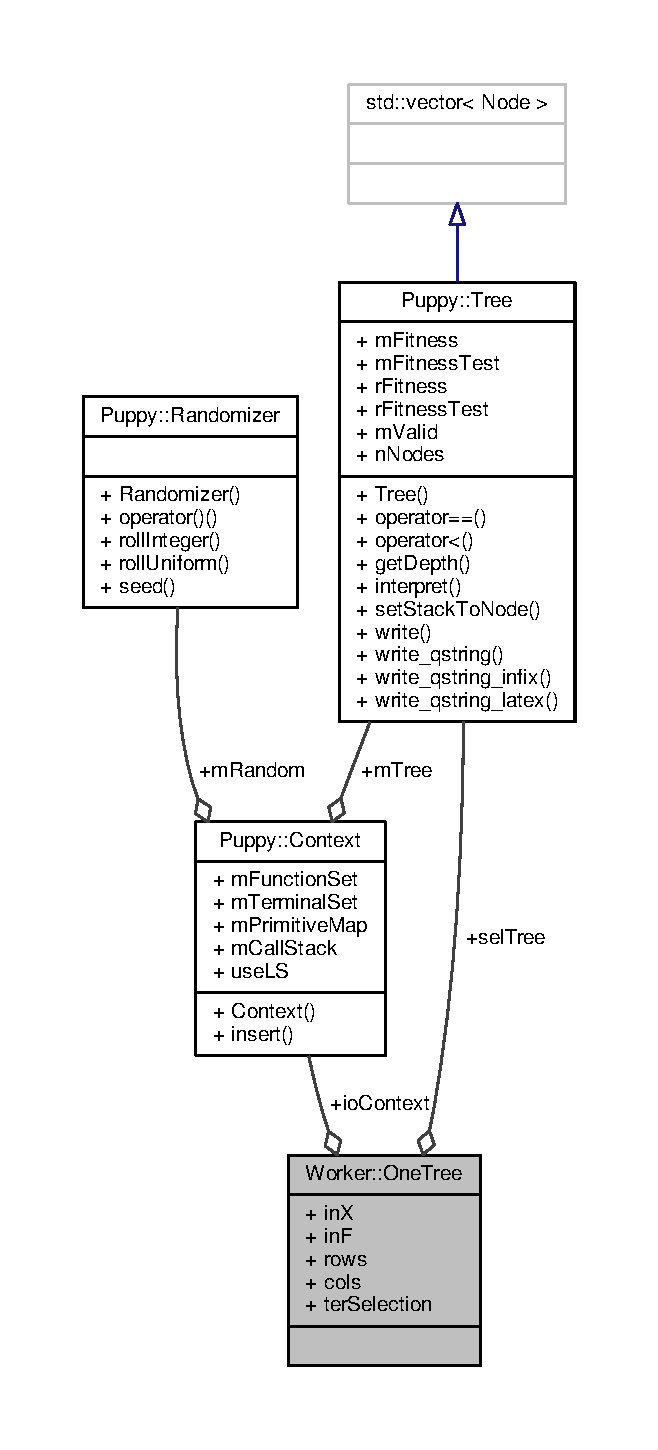
\includegraphics[height=550pt]{structWorker_1_1OneTree__coll__graph}
\end{center}
\end{figure}
\subsection*{Public Attributes}
\begin{DoxyCompactItemize}
\item 
\hypertarget{structWorker_1_1OneTree_ab07dff55ad074fcbec94d809b0edfe8f}{}\hyperlink{classPuppy_1_1Tree}{Puppy\+::\+Tree} {\bfseries sel\+Tree}\label{structWorker_1_1OneTree_ab07dff55ad074fcbec94d809b0edfe8f}

\item 
\hypertarget{structWorker_1_1OneTree_ad999d3b95d626ba7ad697ce26d2a0bf9}{}double $\ast$ {\bfseries in\+X}\label{structWorker_1_1OneTree_ad999d3b95d626ba7ad697ce26d2a0bf9}

\item 
\hypertarget{structWorker_1_1OneTree_a6e05fd4bbc1774fdfc82c2c6e73c4860}{}double $\ast$ {\bfseries in\+F}\label{structWorker_1_1OneTree_a6e05fd4bbc1774fdfc82c2c6e73c4860}

\item 
\hypertarget{structWorker_1_1OneTree_a64d1a9ad0a9cfe03d2225f4e89f8ea53}{}int {\bfseries rows}\label{structWorker_1_1OneTree_a64d1a9ad0a9cfe03d2225f4e89f8ea53}

\item 
\hypertarget{structWorker_1_1OneTree_ac75b7812f9012c9695742f268e991fa6}{}int {\bfseries cols}\label{structWorker_1_1OneTree_ac75b7812f9012c9695742f268e991fa6}

\item 
\hypertarget{structWorker_1_1OneTree_a2e846fc526debedcf594ecad18661af5}{}std\+::vector$<$ bool $>$ {\bfseries ter\+Selection}\label{structWorker_1_1OneTree_a2e846fc526debedcf594ecad18661af5}

\item 
\hypertarget{structWorker_1_1OneTree_aa7c4ca8e12cd50f01c3df2daf380415b}{}\hyperlink{classPuppy_1_1Context}{Puppy\+::\+Context} {\bfseries io\+Context}\label{structWorker_1_1OneTree_aa7c4ca8e12cd50f01c3df2daf380415b}

\end{DoxyCompactItemize}


The documentation for this struct was generated from the following file\+:\begin{DoxyCompactItemize}
\item 
source/worker.\+h\end{DoxyCompactItemize}

\hypertarget{classPuppy_1_1Primitive}{}\section{Puppy\+:\+:Primitive Class Reference}
\label{classPuppy_1_1Primitive}\index{Puppy\+::\+Primitive@{Puppy\+::\+Primitive}}


Genetic programming abstract primitive class.

A primitive is an abstract class of terminals and functions that can be used in a G\+P program. Concrete primitives must define method execute, which define the characteristic operation to execute. Primitives are generally heap allocated (with a call to the new operator) and managed by the associated smart pointer defined in class \hyperlink{classPuppy_1_1PrimitiveHandle}{Primitive\+Handle}.  




Inheritance diagram for Puppy\+:\+:Primitive\+:
\nopagebreak
\begin{figure}[H]
\begin{center}
\leavevmode
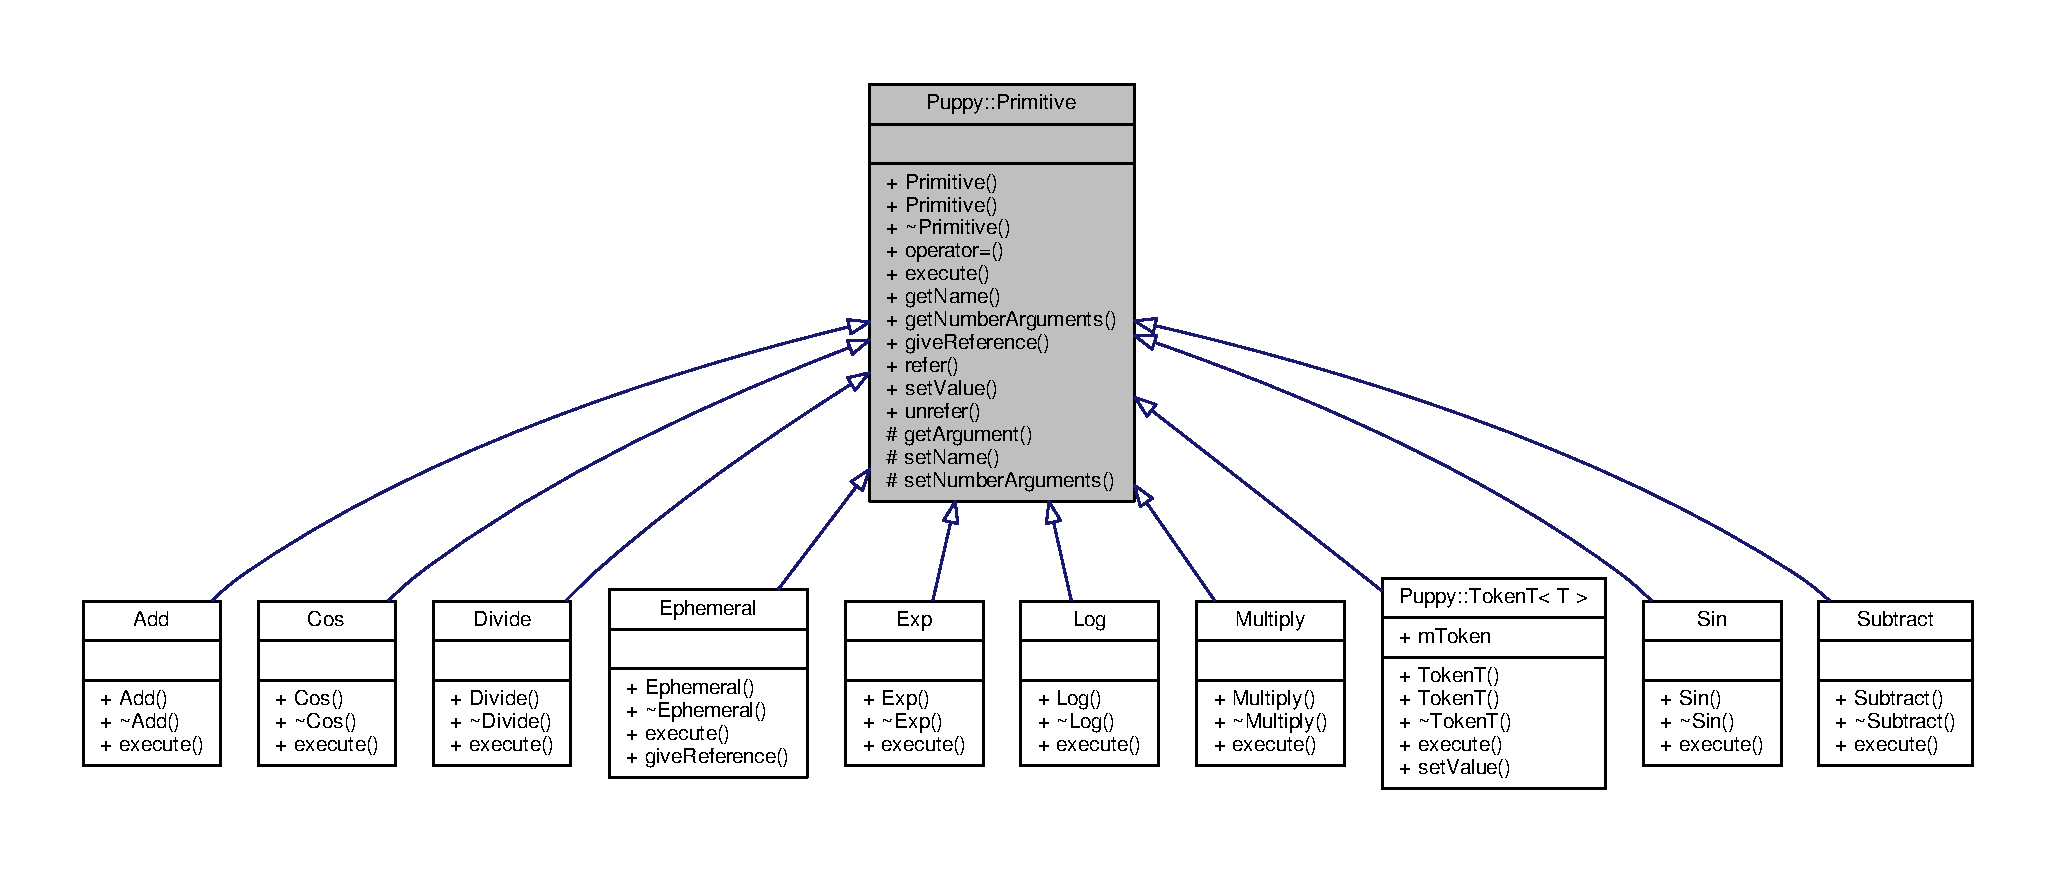
\includegraphics[width=350pt]{classPuppy_1_1Primitive__inherit__graph}
\end{center}
\end{figure}


Collaboration diagram for Puppy\+:\+:Primitive\+:
\nopagebreak
\begin{figure}[H]
\begin{center}
\leavevmode
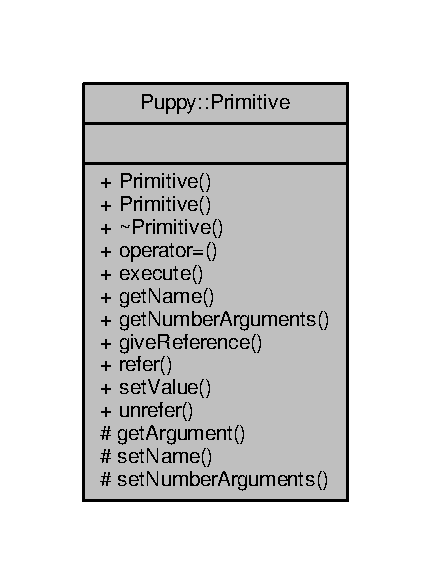
\includegraphics[width=207pt]{classPuppy_1_1Primitive__coll__graph}
\end{center}
\end{figure}
\subsection*{Public Member Functions}
\begin{DoxyCompactItemize}
\item 
\hyperlink{classPuppy_1_1Primitive_a17fd0027a0723bcb35b98f1b43eebeb6}{Primitive} (unsigned int in\+Number\+Arguments=0, std\+::string in\+Name=\char`\"{}\char`\"{})
\begin{DoxyCompactList}\small\item\em Construct a primitive. \end{DoxyCompactList}\item 
\hyperlink{classPuppy_1_1Primitive_a3b3d62da2d801dd5c1e7d6dd532bf45d}{Primitive} (const \hyperlink{classPuppy_1_1Primitive}{Primitive} \&in\+Right\+Primit)
\begin{DoxyCompactList}\small\item\em Copy-\/construct a primitive. \end{DoxyCompactList}\item 
\hyperlink{classPuppy_1_1Primitive}{Primitive} \& \hyperlink{classPuppy_1_1Primitive_a6b93a819ffca6451f44babace6df562a}{operator=} (const \hyperlink{classPuppy_1_1Primitive}{Primitive} \&in\+Right\+Primit)
\begin{DoxyCompactList}\small\item\em Copy a primitive. \end{DoxyCompactList}\item 
virtual void \hyperlink{classPuppy_1_1Primitive_aaef85034e66f49903c591158c3b5ffef}{execute} (void $\ast$out\+Datum, \hyperlink{classPuppy_1_1Context}{Context} \&io\+Context)=0
\begin{DoxyCompactList}\small\item\em Execute the caracteristic primitive operation. \end{DoxyCompactList}\item 
std\+::string \hyperlink{classPuppy_1_1Primitive_a54739a2bb20095ba3a870d5a0f40ce97}{get\+Name} () const 
\begin{DoxyCompactList}\small\item\em Get the name of the primitive. \end{DoxyCompactList}\item 
unsigned int \hyperlink{classPuppy_1_1Primitive_abddcfecae834ed4ad1e4ef0f21c4a3ff}{get\+Number\+Arguments} () const 
\begin{DoxyCompactList}\small\item\em Get the number of arguments of the primitive. \end{DoxyCompactList}\item 
virtual \hyperlink{classPuppy_1_1PrimitiveHandle}{Primitive\+Handle} \hyperlink{classPuppy_1_1Primitive_a0319f5a18dd42fe96c77c895948acc2a}{give\+Reference} (\hyperlink{classPuppy_1_1Context}{Context} \&io\+Context)
\begin{DoxyCompactList}\small\item\em Give a reference on the actual primitive. \end{DoxyCompactList}\item 
\hyperlink{classPuppy_1_1Primitive}{Primitive} $\ast$ \hyperlink{classPuppy_1_1Primitive_abc05de8e8a0d2106ae78637a4785a46d}{refer} ()
\begin{DoxyCompactList}\small\item\em Increments the reference counter and returns a pointer to the actual primitive. \end{DoxyCompactList}\item 
virtual void \hyperlink{classPuppy_1_1Primitive_a2cd429caecd22c31166230b3467fb861}{set\+Value} (const void $\ast$in\+Value)
\begin{DoxyCompactList}\small\item\em Set the value of the primitive (do nothing for basic primitive). \end{DoxyCompactList}\item 
\hypertarget{classPuppy_1_1Primitive_aa8d8f10165e9f6d8cfa158be32e00a79}{}void \hyperlink{classPuppy_1_1Primitive_aa8d8f10165e9f6d8cfa158be32e00a79}{unrefer} ()\label{classPuppy_1_1Primitive_aa8d8f10165e9f6d8cfa158be32e00a79}

\begin{DoxyCompactList}\small\item\em Decrement the reference counter and deletes the actual primitive if it reaches zero. \end{DoxyCompactList}\end{DoxyCompactItemize}
\subsection*{Protected Member Functions}
\begin{DoxyCompactItemize}
\item 
void \hyperlink{classPuppy_1_1Primitive_a908bba73fb1b2df6c708c0235381bbac}{get\+Argument} (unsigned int in\+N, void $\ast$out\+Result, \hyperlink{classPuppy_1_1Context}{Context} \&io\+Context)
\begin{DoxyCompactList}\small\item\em Get the value of the nth argument. \end{DoxyCompactList}\item 
void \hyperlink{classPuppy_1_1Primitive_ae371fdd5d7c917f5fe0826e08f04ad11}{set\+Name} (std\+::string in\+Name)
\begin{DoxyCompactList}\small\item\em Set the name of the primitive. \end{DoxyCompactList}\item 
void \hyperlink{classPuppy_1_1Primitive_a11bb487496584214eb627bf6ae03fad2}{set\+Number\+Arguments} (unsigned int in\+Number\+Arguments)
\begin{DoxyCompactList}\small\item\em Set the number of arguments of the primitive. \end{DoxyCompactList}\end{DoxyCompactItemize}


\subsection{Detailed Description}
Genetic programming abstract primitive class.

A primitive is an abstract class of terminals and functions that can be used in a G\+P program. Concrete primitives must define method execute, which define the characteristic operation to execute. Primitives are generally heap allocated (with a call to the new operator) and managed by the associated smart pointer defined in class \hyperlink{classPuppy_1_1PrimitiveHandle}{Primitive\+Handle}. 

\subsection{Constructor \& Destructor Documentation}
\hypertarget{classPuppy_1_1Primitive_a17fd0027a0723bcb35b98f1b43eebeb6}{}\index{Puppy\+::\+Primitive@{Puppy\+::\+Primitive}!Primitive@{Primitive}}
\index{Primitive@{Primitive}!Puppy\+::\+Primitive@{Puppy\+::\+Primitive}}
\subsubsection[{Primitive}]{\setlength{\rightskip}{0pt plus 5cm}Puppy\+::\+Primitive\+::\+Primitive (
\begin{DoxyParamCaption}
\item[{unsigned int}]{in\+Number\+Arguments = {\ttfamily 0}, }
\item[{std\+::string}]{in\+Name = {\ttfamily \char`\"{}\char`\"{}}}
\end{DoxyParamCaption}
)\hspace{0.3cm}{\ttfamily [explicit]}}\label{classPuppy_1_1Primitive_a17fd0027a0723bcb35b98f1b43eebeb6}


Construct a primitive. 


\begin{DoxyParams}{Parameters}
{\em in\+Number\+Arguments} & Number of arguments of the primitive. \\
\hline
{\em in\+Name} & Name of the primitive. \\
\hline
\end{DoxyParams}
\hypertarget{classPuppy_1_1Primitive_a3b3d62da2d801dd5c1e7d6dd532bf45d}{}\index{Puppy\+::\+Primitive@{Puppy\+::\+Primitive}!Primitive@{Primitive}}
\index{Primitive@{Primitive}!Puppy\+::\+Primitive@{Puppy\+::\+Primitive}}
\subsubsection[{Primitive}]{\setlength{\rightskip}{0pt plus 5cm}Puppy\+::\+Primitive\+::\+Primitive (
\begin{DoxyParamCaption}
\item[{const {\bf Primitive} \&}]{in\+Right\+Primit}
\end{DoxyParamCaption}
)}\label{classPuppy_1_1Primitive_a3b3d62da2d801dd5c1e7d6dd532bf45d}


Copy-\/construct a primitive. 


\begin{DoxyParams}{Parameters}
{\em in\+Right\+Primit} & \hyperlink{classPuppy_1_1Primitive}{Primitive} to copy. \\
\hline
\end{DoxyParams}


\subsection{Member Function Documentation}
\hypertarget{classPuppy_1_1Primitive_aaef85034e66f49903c591158c3b5ffef}{}\index{Puppy\+::\+Primitive@{Puppy\+::\+Primitive}!execute@{execute}}
\index{execute@{execute}!Puppy\+::\+Primitive@{Puppy\+::\+Primitive}}
\subsubsection[{execute}]{\setlength{\rightskip}{0pt plus 5cm}virtual void Puppy\+::\+Primitive\+::execute (
\begin{DoxyParamCaption}
\item[{void $\ast$}]{out\+Datum, }
\item[{{\bf Context} \&}]{io\+Context}
\end{DoxyParamCaption}
)\hspace{0.3cm}{\ttfamily [pure virtual]}}\label{classPuppy_1_1Primitive_aaef85034e66f49903c591158c3b5ffef}


Execute the caracteristic primitive operation. 


\begin{DoxyParams}{Parameters}
{\em out\+Datum} & Result of the execution. \\
\hline
{\em io\+Context} & Evolutionary context. \\
\hline
\end{DoxyParams}


Implemented in \hyperlink{classEphemeral_a69fb1365baddf81c9f1cd7c35a6bad16}{Ephemeral}, \hyperlink{classExp_af04e8771ab5a8b572779d0703efa2736}{Exp}, \hyperlink{classLog_a0f034cdf9ef168f4ee556e24934519ab}{Log}, \hyperlink{classCos_ae797f1f97801e6a64e4bded4f4f4f263}{Cos}, \hyperlink{classSin_a52e8e8096eb90f30418dc74e0a89a1ec}{Sin}, \hyperlink{classDivide_af5ed152cd9a4e65141a59ef78307e87f}{Divide}, \hyperlink{classMultiply_a965412103b5dadd21ed4d58c8d6c6d87}{Multiply}, \hyperlink{classSubtract_a7b85b95cd90fe9633ba684802343d2e2}{Subtract}, \hyperlink{classPuppy_1_1TokenT_a15641f373da2d98c057247c32deb943a}{Puppy\+::\+Token\+T$<$ T $>$}, and \hyperlink{classAdd_a5f17154064fd521553352f114db35018}{Add}.

\hypertarget{classPuppy_1_1Primitive_a908bba73fb1b2df6c708c0235381bbac}{}\index{Puppy\+::\+Primitive@{Puppy\+::\+Primitive}!get\+Argument@{get\+Argument}}
\index{get\+Argument@{get\+Argument}!Puppy\+::\+Primitive@{Puppy\+::\+Primitive}}
\subsubsection[{get\+Argument}]{\setlength{\rightskip}{0pt plus 5cm}void Puppy\+::\+Primitive\+::get\+Argument (
\begin{DoxyParamCaption}
\item[{unsigned int}]{in\+N, }
\item[{void $\ast$}]{out\+Result, }
\item[{{\bf Puppy\+::\+Context} \&}]{io\+Context}
\end{DoxyParamCaption}
)\hspace{0.3cm}{\ttfamily [inline]}, {\ttfamily [protected]}}\label{classPuppy_1_1Primitive_a908bba73fb1b2df6c708c0235381bbac}


Get the value of the nth argument. 


\begin{DoxyParams}{Parameters}
{\em in\+N} & Index of the argument to get. \\
\hline
{\em out\+Result} & Value of the nth argument. \\
\hline
{\em io\+Context} & Evolutionary context. \\
\hline
\end{DoxyParams}
\hypertarget{classPuppy_1_1Primitive_a54739a2bb20095ba3a870d5a0f40ce97}{}\index{Puppy\+::\+Primitive@{Puppy\+::\+Primitive}!get\+Name@{get\+Name}}
\index{get\+Name@{get\+Name}!Puppy\+::\+Primitive@{Puppy\+::\+Primitive}}
\subsubsection[{get\+Name}]{\setlength{\rightskip}{0pt plus 5cm}std\+::string Puppy\+::\+Primitive\+::get\+Name (
\begin{DoxyParamCaption}
{}
\end{DoxyParamCaption}
) const\hspace{0.3cm}{\ttfamily [inline]}}\label{classPuppy_1_1Primitive_a54739a2bb20095ba3a870d5a0f40ce97}


Get the name of the primitive. 

\begin{DoxyReturn}{Returns}
Name of the primitive. 
\end{DoxyReturn}
\hypertarget{classPuppy_1_1Primitive_abddcfecae834ed4ad1e4ef0f21c4a3ff}{}\index{Puppy\+::\+Primitive@{Puppy\+::\+Primitive}!get\+Number\+Arguments@{get\+Number\+Arguments}}
\index{get\+Number\+Arguments@{get\+Number\+Arguments}!Puppy\+::\+Primitive@{Puppy\+::\+Primitive}}
\subsubsection[{get\+Number\+Arguments}]{\setlength{\rightskip}{0pt plus 5cm}unsigned int Puppy\+::\+Primitive\+::get\+Number\+Arguments (
\begin{DoxyParamCaption}
{}
\end{DoxyParamCaption}
) const\hspace{0.3cm}{\ttfamily [inline]}}\label{classPuppy_1_1Primitive_abddcfecae834ed4ad1e4ef0f21c4a3ff}


Get the number of arguments of the primitive. 

\begin{DoxyReturn}{Returns}
Number of arguments of the primitive. 
\end{DoxyReturn}
\hypertarget{classPuppy_1_1Primitive_a0319f5a18dd42fe96c77c895948acc2a}{}\index{Puppy\+::\+Primitive@{Puppy\+::\+Primitive}!give\+Reference@{give\+Reference}}
\index{give\+Reference@{give\+Reference}!Puppy\+::\+Primitive@{Puppy\+::\+Primitive}}
\subsubsection[{give\+Reference}]{\setlength{\rightskip}{0pt plus 5cm}{\bf Puppy\+::\+Primitive\+Handle} Puppy\+::\+Primitive\+::give\+Reference (
\begin{DoxyParamCaption}
\item[{{\bf Puppy\+::\+Context} \&}]{io\+Context}
\end{DoxyParamCaption}
)\hspace{0.3cm}{\ttfamily [virtual]}}\label{classPuppy_1_1Primitive_a0319f5a18dd42fe96c77c895948acc2a}


Give a reference on the actual primitive. 


\begin{DoxyParams}{Parameters}
{\em io\+Context} & Evolutionary context. \\
\hline
\end{DoxyParams}
\begin{DoxyReturn}{Returns}
\hyperlink{classPuppy_1_1Primitive}{Primitive} handle to this pointer. 
\end{DoxyReturn}


Reimplemented in \hyperlink{classEphemeral_a4c8bf775486a868d9011c4b9d93e7547}{Ephemeral}.

\hypertarget{classPuppy_1_1Primitive_a6b93a819ffca6451f44babace6df562a}{}\index{Puppy\+::\+Primitive@{Puppy\+::\+Primitive}!operator=@{operator=}}
\index{operator=@{operator=}!Puppy\+::\+Primitive@{Puppy\+::\+Primitive}}
\subsubsection[{operator=}]{\setlength{\rightskip}{0pt plus 5cm}{\bf Puppy\+::\+Primitive} \& Puppy\+::\+Primitive\+::operator= (
\begin{DoxyParamCaption}
\item[{const {\bf Primitive} \&}]{in\+Right\+Primit}
\end{DoxyParamCaption}
)}\label{classPuppy_1_1Primitive_a6b93a819ffca6451f44babace6df562a}


Copy a primitive. 


\begin{DoxyParams}{Parameters}
{\em in\+Right\+Primit} & \hyperlink{classPuppy_1_1Primitive}{Primitive} to copy. \\
\hline
\end{DoxyParams}
\hypertarget{classPuppy_1_1Primitive_abc05de8e8a0d2106ae78637a4785a46d}{}\index{Puppy\+::\+Primitive@{Puppy\+::\+Primitive}!refer@{refer}}
\index{refer@{refer}!Puppy\+::\+Primitive@{Puppy\+::\+Primitive}}
\subsubsection[{refer}]{\setlength{\rightskip}{0pt plus 5cm}{\bf Puppy\+::\+Primitive} $\ast$ Puppy\+::\+Primitive\+::refer (
\begin{DoxyParamCaption}
{}
\end{DoxyParamCaption}
)\hspace{0.3cm}{\ttfamily [inline]}}\label{classPuppy_1_1Primitive_abc05de8e8a0d2106ae78637a4785a46d}


Increments the reference counter and returns a pointer to the actual primitive. 

\begin{DoxyReturn}{Returns}
Pointer to the actual primitive. 
\end{DoxyReturn}
\hypertarget{classPuppy_1_1Primitive_ae371fdd5d7c917f5fe0826e08f04ad11}{}\index{Puppy\+::\+Primitive@{Puppy\+::\+Primitive}!set\+Name@{set\+Name}}
\index{set\+Name@{set\+Name}!Puppy\+::\+Primitive@{Puppy\+::\+Primitive}}
\subsubsection[{set\+Name}]{\setlength{\rightskip}{0pt plus 5cm}void Puppy\+::\+Primitive\+::set\+Name (
\begin{DoxyParamCaption}
\item[{std\+::string}]{in\+Name}
\end{DoxyParamCaption}
)\hspace{0.3cm}{\ttfamily [protected]}}\label{classPuppy_1_1Primitive_ae371fdd5d7c917f5fe0826e08f04ad11}


Set the name of the primitive. 


\begin{DoxyParams}{Parameters}
{\em in\+Name} & Name of the primitive. \\
\hline
\end{DoxyParams}
\hypertarget{classPuppy_1_1Primitive_a11bb487496584214eb627bf6ae03fad2}{}\index{Puppy\+::\+Primitive@{Puppy\+::\+Primitive}!set\+Number\+Arguments@{set\+Number\+Arguments}}
\index{set\+Number\+Arguments@{set\+Number\+Arguments}!Puppy\+::\+Primitive@{Puppy\+::\+Primitive}}
\subsubsection[{set\+Number\+Arguments}]{\setlength{\rightskip}{0pt plus 5cm}void Puppy\+::\+Primitive\+::set\+Number\+Arguments (
\begin{DoxyParamCaption}
\item[{unsigned int}]{in\+Number\+Arguments}
\end{DoxyParamCaption}
)\hspace{0.3cm}{\ttfamily [protected]}}\label{classPuppy_1_1Primitive_a11bb487496584214eb627bf6ae03fad2}


Set the number of arguments of the primitive. 


\begin{DoxyParams}{Parameters}
{\em in\+Number\+Arguments} & Number of arguments of the primitive. \\
\hline
\end{DoxyParams}
\hypertarget{classPuppy_1_1Primitive_a2cd429caecd22c31166230b3467fb861}{}\index{Puppy\+::\+Primitive@{Puppy\+::\+Primitive}!set\+Value@{set\+Value}}
\index{set\+Value@{set\+Value}!Puppy\+::\+Primitive@{Puppy\+::\+Primitive}}
\subsubsection[{set\+Value}]{\setlength{\rightskip}{0pt plus 5cm}void Puppy\+::\+Primitive\+::set\+Value (
\begin{DoxyParamCaption}
\item[{const void $\ast$}]{in\+Value}
\end{DoxyParamCaption}
)\hspace{0.3cm}{\ttfamily [virtual]}}\label{classPuppy_1_1Primitive_a2cd429caecd22c31166230b3467fb861}


Set the value of the primitive (do nothing for basic primitive). 


\begin{DoxyParams}{Parameters}
{\em in\+Value} & New value to use. \\
\hline
\end{DoxyParams}


Reimplemented in \hyperlink{classPuppy_1_1TokenT_ad38ced7ce46e1ef1449bd90560296f3f}{Puppy\+::\+Token\+T$<$ T $>$}.



The documentation for this class was generated from the following files\+:\begin{DoxyCompactItemize}
\item 
source/puppy\+\_\+primitive.\+hpp\item 
source/puppy\+\_\+primitive.\+cpp\item 
source/puppy\+\_\+primitiveinline.\+hpp\end{DoxyCompactItemize}

\hypertarget{classPuppy_1_1PrimitiveHandle}{}\section{Puppy\+:\+:Primitive\+Handle Class Reference}
\label{classPuppy_1_1PrimitiveHandle}\index{Puppy\+::\+Primitive\+Handle@{Puppy\+::\+Primitive\+Handle}}


Smart pointer to a primitive.

\hyperlink{classPuppy_1_1Primitive}{Primitive} handle defines a smart pointer to a primitive. It behaves much like a standard pointer, but it also call the appriate refer and unrefer methods of class primitive.  




Collaboration diagram for Puppy\+:\+:Primitive\+Handle\+:
\nopagebreak
\begin{figure}[H]
\begin{center}
\leavevmode
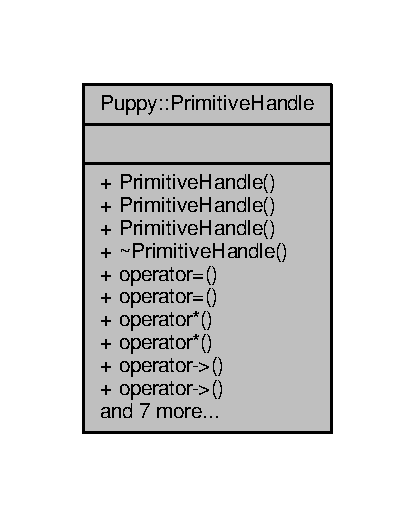
\includegraphics[width=199pt]{classPuppy_1_1PrimitiveHandle__coll__graph}
\end{center}
\end{figure}
\subsection*{Public Member Functions}
\begin{DoxyCompactItemize}
\item 
\hypertarget{classPuppy_1_1PrimitiveHandle_afc2b75ba067b8030f997dfd1577ad189}{}\hyperlink{classPuppy_1_1PrimitiveHandle_afc2b75ba067b8030f997dfd1577ad189}{Primitive\+Handle} ()\label{classPuppy_1_1PrimitiveHandle_afc2b75ba067b8030f997dfd1577ad189}

\begin{DoxyCompactList}\small\item\em Construct a N\+U\+L\+L pointing primitive smart \hyperlink{classPuppy_1_1PrimitiveHandle}{Primitive\+Handle}. \end{DoxyCompactList}\item 
\hyperlink{classPuppy_1_1PrimitiveHandle_adfe32a81fdb0ff32a4bc9be018944531}{Primitive\+Handle} (const \hyperlink{classPuppy_1_1Primitive}{Primitive} $\ast$in\+Primit\+Ptr)
\begin{DoxyCompactList}\small\item\em Construct a primitive smart pointer that refer to the object pointed given. \end{DoxyCompactList}\item 
\hyperlink{classPuppy_1_1PrimitiveHandle_aa512ff37494d12d450b61814827939b3}{Primitive\+Handle} (const \hyperlink{classPuppy_1_1PrimitiveHandle}{Primitive\+Handle} \&in\+Primitive\+Handle)
\begin{DoxyCompactList}\small\item\em Copy construct a primitive smart pointer. \end{DoxyCompactList}\item 
\hypertarget{classPuppy_1_1PrimitiveHandle_a8554d88db5964a0a6b125360c97efc44}{}\hyperlink{classPuppy_1_1PrimitiveHandle_a8554d88db5964a0a6b125360c97efc44}{$\sim$\+Primitive\+Handle} ()\label{classPuppy_1_1PrimitiveHandle_a8554d88db5964a0a6b125360c97efc44}

\begin{DoxyCompactList}\small\item\em Destruct a primitive smart pointer by unrefering the pointed object. \end{DoxyCompactList}\item 
\hyperlink{classPuppy_1_1PrimitiveHandle}{Primitive\+Handle} \& \hyperlink{classPuppy_1_1PrimitiveHandle_a1aaf940a337bebe97f80aa4d7fe9d451}{operator=} (const \hyperlink{classPuppy_1_1Primitive}{Primitive} $\ast$in\+Primit\+Ptr)
\begin{DoxyCompactList}\small\item\em Affect the actual \hyperlink{classPuppy_1_1PrimitiveHandle}{Primitive\+Handle} to an object \hyperlink{classPuppy_1_1PrimitiveHandle}{Primitive\+Handle}. \end{DoxyCompactList}\item 
\hyperlink{classPuppy_1_1PrimitiveHandle}{Primitive\+Handle} \& \hyperlink{classPuppy_1_1PrimitiveHandle_ad35a2449566fb91ff70feca52cc9a738}{operator=} (const \hyperlink{classPuppy_1_1PrimitiveHandle}{Primitive\+Handle} \&in\+Primitive\+Handle)
\begin{DoxyCompactList}\small\item\em Affect the actual pointer to another smart pointer. \end{DoxyCompactList}\item 
\hyperlink{classPuppy_1_1Primitive}{Primitive} \& \hyperlink{classPuppy_1_1PrimitiveHandle_ada654223700c4b57e63a338804ac3c9f}{operator$\ast$} ()
\begin{DoxyCompactList}\small\item\em Get reference the primitive pointed. \end{DoxyCompactList}\item 
const \hyperlink{classPuppy_1_1Primitive}{Primitive} \& \hyperlink{classPuppy_1_1PrimitiveHandle_a265e0c2a791fd2deef5b543f5ccc2e44}{operator$\ast$} () const 
\begin{DoxyCompactList}\small\item\em Get constant reference the primitive pointed. \end{DoxyCompactList}\item 
\hyperlink{classPuppy_1_1Primitive}{Primitive} $\ast$ \hyperlink{classPuppy_1_1PrimitiveHandle_a64dbf49fabd8c7cd499ed44d1c77c718}{operator-\/$>$} ()
\begin{DoxyCompactList}\small\item\em Get reference the primitive pointed. \end{DoxyCompactList}\item 
const \hyperlink{classPuppy_1_1Primitive}{Primitive} $\ast$ \hyperlink{classPuppy_1_1PrimitiveHandle_a96bc2d4e05e7456402dab94954e3aa19}{operator-\/$>$} () const 
\begin{DoxyCompactList}\small\item\em Get constant reference the primitive pointed. \end{DoxyCompactList}\item 
bool \hyperlink{classPuppy_1_1PrimitiveHandle_ae4a43e20e9fed246e3ccf4db0a2a4821}{operator!} () const 
\begin{DoxyCompactList}\small\item\em Test whether the pointer is N\+U\+L\+L or not. \end{DoxyCompactList}\item 
bool \hyperlink{classPuppy_1_1PrimitiveHandle_a79bbe9c55a986778965a63c1e3c39f7b}{operator==} (const \hyperlink{classPuppy_1_1Primitive}{Primitive} $\ast$in\+Primit\+Ptr) const 
\begin{DoxyCompactList}\small\item\em Compare a smart pointer to a primitive pointer. \end{DoxyCompactList}\item 
bool \hyperlink{classPuppy_1_1PrimitiveHandle_ad9ec731cb2abe6248499ea2e8d273c31}{operator==} (const \hyperlink{classPuppy_1_1PrimitiveHandle}{Primitive\+Handle} \&in\+Primitive\+Handle) const 
\begin{DoxyCompactList}\small\item\em Compare two primitive smart pointer. \end{DoxyCompactList}\item 
bool \hyperlink{classPuppy_1_1PrimitiveHandle_a378f6a3e812a17eb7405edeebec0403d}{operator!=} (const \hyperlink{classPuppy_1_1Primitive}{Primitive} $\ast$in\+Primit\+Ptr) const 
\begin{DoxyCompactList}\small\item\em Compare a smart pointer to a primitive pointer. \end{DoxyCompactList}\item 
bool \hyperlink{classPuppy_1_1PrimitiveHandle_a58698eef8cf454f72eeadc62da386558}{operator!=} (const \hyperlink{classPuppy_1_1PrimitiveHandle}{Primitive\+Handle} \&in\+Primitive\+Handle) const 
\begin{DoxyCompactList}\small\item\em Compare two smart Primitive\+Handles. \end{DoxyCompactList}\item 
\hyperlink{classPuppy_1_1Primitive}{Primitive} $\ast$ \hyperlink{classPuppy_1_1PrimitiveHandle_a058132aa2eb92bbc05fc03a62431103e}{get\+Pointer} ()
\begin{DoxyCompactList}\small\item\em Return pointer to the referenced primitive. \end{DoxyCompactList}\item 
const \hyperlink{classPuppy_1_1Primitive}{Primitive} $\ast$ \hyperlink{classPuppy_1_1PrimitiveHandle_a2a90e66dd41ca18f4937eceb523cb572}{get\+Pointer} () const 
\begin{DoxyCompactList}\small\item\em Return constant pointer to the referenced primitive. \end{DoxyCompactList}\end{DoxyCompactItemize}


\subsection{Detailed Description}
Smart pointer to a primitive.

\hyperlink{classPuppy_1_1Primitive}{Primitive} handle defines a smart pointer to a primitive. It behaves much like a standard pointer, but it also call the appriate refer and unrefer methods of class primitive. 

\subsection{Constructor \& Destructor Documentation}
\hypertarget{classPuppy_1_1PrimitiveHandle_adfe32a81fdb0ff32a4bc9be018944531}{}\index{Puppy\+::\+Primitive\+Handle@{Puppy\+::\+Primitive\+Handle}!Primitive\+Handle@{Primitive\+Handle}}
\index{Primitive\+Handle@{Primitive\+Handle}!Puppy\+::\+Primitive\+Handle@{Puppy\+::\+Primitive\+Handle}}
\subsubsection[{Primitive\+Handle}]{\setlength{\rightskip}{0pt plus 5cm}Puppy\+::\+Primitive\+Handle\+::\+Primitive\+Handle (
\begin{DoxyParamCaption}
\item[{const {\bf Primitive} $\ast$}]{in\+Primit\+Ptr}
\end{DoxyParamCaption}
)\hspace{0.3cm}{\ttfamily [inline]}}\label{classPuppy_1_1PrimitiveHandle_adfe32a81fdb0ff32a4bc9be018944531}


Construct a primitive smart pointer that refer to the object pointed given. 


\begin{DoxyParams}{Parameters}
{\em in\+Primit\+Ptr} & Pointer to the object to be referenced. \\
\hline
\end{DoxyParams}
\hypertarget{classPuppy_1_1PrimitiveHandle_aa512ff37494d12d450b61814827939b3}{}\index{Puppy\+::\+Primitive\+Handle@{Puppy\+::\+Primitive\+Handle}!Primitive\+Handle@{Primitive\+Handle}}
\index{Primitive\+Handle@{Primitive\+Handle}!Puppy\+::\+Primitive\+Handle@{Puppy\+::\+Primitive\+Handle}}
\subsubsection[{Primitive\+Handle}]{\setlength{\rightskip}{0pt plus 5cm}Puppy\+::\+Primitive\+Handle\+::\+Primitive\+Handle (
\begin{DoxyParamCaption}
\item[{const {\bf Primitive\+Handle} \&}]{in\+Primitive\+Handle}
\end{DoxyParamCaption}
)\hspace{0.3cm}{\ttfamily [inline]}}\label{classPuppy_1_1PrimitiveHandle_aa512ff37494d12d450b61814827939b3}


Copy construct a primitive smart pointer. 


\begin{DoxyParams}{Parameters}
{\em in\+Primitive\+Handle} & Smart \hyperlink{classPuppy_1_1PrimitiveHandle}{Primitive\+Handle} to copy. \\
\hline
\end{DoxyParams}


\subsection{Member Function Documentation}
\hypertarget{classPuppy_1_1PrimitiveHandle_a058132aa2eb92bbc05fc03a62431103e}{}\index{Puppy\+::\+Primitive\+Handle@{Puppy\+::\+Primitive\+Handle}!get\+Pointer@{get\+Pointer}}
\index{get\+Pointer@{get\+Pointer}!Puppy\+::\+Primitive\+Handle@{Puppy\+::\+Primitive\+Handle}}
\subsubsection[{get\+Pointer}]{\setlength{\rightskip}{0pt plus 5cm}{\bf Puppy\+::\+Primitive} $\ast$ Puppy\+::\+Primitive\+Handle\+::get\+Pointer (
\begin{DoxyParamCaption}
{}
\end{DoxyParamCaption}
)\hspace{0.3cm}{\ttfamily [inline]}}\label{classPuppy_1_1PrimitiveHandle_a058132aa2eb92bbc05fc03a62431103e}


Return pointer to the referenced primitive. 

\begin{DoxyReturn}{Returns}
C++ pointer to the primitive. 
\end{DoxyReturn}
\hypertarget{classPuppy_1_1PrimitiveHandle_a2a90e66dd41ca18f4937eceb523cb572}{}\index{Puppy\+::\+Primitive\+Handle@{Puppy\+::\+Primitive\+Handle}!get\+Pointer@{get\+Pointer}}
\index{get\+Pointer@{get\+Pointer}!Puppy\+::\+Primitive\+Handle@{Puppy\+::\+Primitive\+Handle}}
\subsubsection[{get\+Pointer}]{\setlength{\rightskip}{0pt plus 5cm}const {\bf Puppy\+::\+Primitive} $\ast$ Puppy\+::\+Primitive\+Handle\+::get\+Pointer (
\begin{DoxyParamCaption}
{}
\end{DoxyParamCaption}
) const\hspace{0.3cm}{\ttfamily [inline]}}\label{classPuppy_1_1PrimitiveHandle_a2a90e66dd41ca18f4937eceb523cb572}


Return constant pointer to the referenced primitive. 

\begin{DoxyReturn}{Returns}
Constant C++ pointer to the primitive. 
\end{DoxyReturn}
\hypertarget{classPuppy_1_1PrimitiveHandle_ae4a43e20e9fed246e3ccf4db0a2a4821}{}\index{Puppy\+::\+Primitive\+Handle@{Puppy\+::\+Primitive\+Handle}!operator"!@{operator"!}}
\index{operator"!@{operator"!}!Puppy\+::\+Primitive\+Handle@{Puppy\+::\+Primitive\+Handle}}
\subsubsection[{operator"!}]{\setlength{\rightskip}{0pt plus 5cm}bool Puppy\+::\+Primitive\+Handle\+::operator! (
\begin{DoxyParamCaption}
{}
\end{DoxyParamCaption}
) const\hspace{0.3cm}{\ttfamily [inline]}}\label{classPuppy_1_1PrimitiveHandle_ae4a43e20e9fed246e3ccf4db0a2a4821}


Test whether the pointer is N\+U\+L\+L or not. 

\begin{DoxyReturn}{Returns}
True if the pointer is N\+U\+L\+L, false if it is not. 
\end{DoxyReturn}
\hypertarget{classPuppy_1_1PrimitiveHandle_a378f6a3e812a17eb7405edeebec0403d}{}\index{Puppy\+::\+Primitive\+Handle@{Puppy\+::\+Primitive\+Handle}!operator"!=@{operator"!=}}
\index{operator"!=@{operator"!=}!Puppy\+::\+Primitive\+Handle@{Puppy\+::\+Primitive\+Handle}}
\subsubsection[{operator"!=}]{\setlength{\rightskip}{0pt plus 5cm}bool {\bf Puppy\+::\+Primitive\+Handle\+::operator!}= (
\begin{DoxyParamCaption}
\item[{const {\bf Primitive} $\ast$}]{in\+Primit\+Ptr}
\end{DoxyParamCaption}
) const\hspace{0.3cm}{\ttfamily [inline]}}\label{classPuppy_1_1PrimitiveHandle_a378f6a3e812a17eb7405edeebec0403d}


Compare a smart pointer to a primitive pointer. 


\begin{DoxyParams}{Parameters}
{\em in\+Primit\+Ptr} & Right hand side primitive pointer to compare. \\
\hline
\end{DoxyParams}
\begin{DoxyReturn}{Returns}
False if they both refer to the same object (or are both N\+U\+L\+L), true if not. 
\end{DoxyReturn}
\hypertarget{classPuppy_1_1PrimitiveHandle_a58698eef8cf454f72eeadc62da386558}{}\index{Puppy\+::\+Primitive\+Handle@{Puppy\+::\+Primitive\+Handle}!operator"!=@{operator"!=}}
\index{operator"!=@{operator"!=}!Puppy\+::\+Primitive\+Handle@{Puppy\+::\+Primitive\+Handle}}
\subsubsection[{operator"!=}]{\setlength{\rightskip}{0pt plus 5cm}bool {\bf Puppy\+::\+Primitive\+Handle\+::operator!}= (
\begin{DoxyParamCaption}
\item[{const {\bf Primitive\+Handle} \&}]{in\+Primitive\+Handle}
\end{DoxyParamCaption}
) const\hspace{0.3cm}{\ttfamily [inline]}}\label{classPuppy_1_1PrimitiveHandle_a58698eef8cf454f72eeadc62da386558}


Compare two smart Primitive\+Handles. 


\begin{DoxyParams}{Parameters}
{\em in\+Primitive\+Handle} & Right hand side smart \hyperlink{classPuppy_1_1PrimitiveHandle}{Primitive\+Handle} to compare. \\
\hline
\end{DoxyParams}
\begin{DoxyReturn}{Returns}
False if they both refer to the same object (or are both N\+U\+L\+L), true if not. 
\end{DoxyReturn}
\hypertarget{classPuppy_1_1PrimitiveHandle_ada654223700c4b57e63a338804ac3c9f}{}\index{Puppy\+::\+Primitive\+Handle@{Puppy\+::\+Primitive\+Handle}!operator$\ast$@{operator$\ast$}}
\index{operator$\ast$@{operator$\ast$}!Puppy\+::\+Primitive\+Handle@{Puppy\+::\+Primitive\+Handle}}
\subsubsection[{operator$\ast$}]{\setlength{\rightskip}{0pt plus 5cm}{\bf Puppy\+::\+Primitive} \& Puppy\+::\+Primitive\+Handle\+::operator$\ast$ (
\begin{DoxyParamCaption}
{}
\end{DoxyParamCaption}
)\hspace{0.3cm}{\ttfamily [inline]}}\label{classPuppy_1_1PrimitiveHandle_ada654223700c4b57e63a338804ac3c9f}


Get reference the primitive pointed. 

\begin{DoxyReturn}{Returns}
Reference to the primitive pointed. 
\end{DoxyReturn}
\hypertarget{classPuppy_1_1PrimitiveHandle_a265e0c2a791fd2deef5b543f5ccc2e44}{}\index{Puppy\+::\+Primitive\+Handle@{Puppy\+::\+Primitive\+Handle}!operator$\ast$@{operator$\ast$}}
\index{operator$\ast$@{operator$\ast$}!Puppy\+::\+Primitive\+Handle@{Puppy\+::\+Primitive\+Handle}}
\subsubsection[{operator$\ast$}]{\setlength{\rightskip}{0pt plus 5cm}const {\bf Puppy\+::\+Primitive} \& Puppy\+::\+Primitive\+Handle\+::operator$\ast$ (
\begin{DoxyParamCaption}
{}
\end{DoxyParamCaption}
) const\hspace{0.3cm}{\ttfamily [inline]}}\label{classPuppy_1_1PrimitiveHandle_a265e0c2a791fd2deef5b543f5ccc2e44}


Get constant reference the primitive pointed. 

\begin{DoxyReturn}{Returns}
Constant reference to the primitive pointed. 
\end{DoxyReturn}
\hypertarget{classPuppy_1_1PrimitiveHandle_a64dbf49fabd8c7cd499ed44d1c77c718}{}\index{Puppy\+::\+Primitive\+Handle@{Puppy\+::\+Primitive\+Handle}!operator-\/$>$@{operator-\/$>$}}
\index{operator-\/$>$@{operator-\/$>$}!Puppy\+::\+Primitive\+Handle@{Puppy\+::\+Primitive\+Handle}}
\subsubsection[{operator-\/$>$}]{\setlength{\rightskip}{0pt plus 5cm}{\bf Puppy\+::\+Primitive} $\ast$ Puppy\+::\+Primitive\+Handle\+::operator-\/$>$ (
\begin{DoxyParamCaption}
{}
\end{DoxyParamCaption}
)\hspace{0.3cm}{\ttfamily [inline]}}\label{classPuppy_1_1PrimitiveHandle_a64dbf49fabd8c7cd499ed44d1c77c718}


Get reference the primitive pointed. 

\begin{DoxyReturn}{Returns}
\hyperlink{classPuppy_1_1PrimitiveHandle}{Primitive\+Handle} to the object pointed. 
\end{DoxyReturn}
\hypertarget{classPuppy_1_1PrimitiveHandle_a96bc2d4e05e7456402dab94954e3aa19}{}\index{Puppy\+::\+Primitive\+Handle@{Puppy\+::\+Primitive\+Handle}!operator-\/$>$@{operator-\/$>$}}
\index{operator-\/$>$@{operator-\/$>$}!Puppy\+::\+Primitive\+Handle@{Puppy\+::\+Primitive\+Handle}}
\subsubsection[{operator-\/$>$}]{\setlength{\rightskip}{0pt plus 5cm}const {\bf Puppy\+::\+Primitive} $\ast$ Puppy\+::\+Primitive\+Handle\+::operator-\/$>$ (
\begin{DoxyParamCaption}
{}
\end{DoxyParamCaption}
) const\hspace{0.3cm}{\ttfamily [inline]}}\label{classPuppy_1_1PrimitiveHandle_a96bc2d4e05e7456402dab94954e3aa19}


Get constant reference the primitive pointed. 

\begin{DoxyReturn}{Returns}
Constant pointer to the primitive pointed. 
\end{DoxyReturn}
\hypertarget{classPuppy_1_1PrimitiveHandle_a1aaf940a337bebe97f80aa4d7fe9d451}{}\index{Puppy\+::\+Primitive\+Handle@{Puppy\+::\+Primitive\+Handle}!operator=@{operator=}}
\index{operator=@{operator=}!Puppy\+::\+Primitive\+Handle@{Puppy\+::\+Primitive\+Handle}}
\subsubsection[{operator=}]{\setlength{\rightskip}{0pt plus 5cm}{\bf Puppy\+::\+Primitive\+Handle} \& Puppy\+::\+Primitive\+Handle\+::operator= (
\begin{DoxyParamCaption}
\item[{const {\bf Primitive} $\ast$}]{in\+Primit\+Ptr}
\end{DoxyParamCaption}
)\hspace{0.3cm}{\ttfamily [inline]}}\label{classPuppy_1_1PrimitiveHandle_a1aaf940a337bebe97f80aa4d7fe9d451}


Affect the actual \hyperlink{classPuppy_1_1PrimitiveHandle}{Primitive\+Handle} to an object \hyperlink{classPuppy_1_1PrimitiveHandle}{Primitive\+Handle}. 


\begin{DoxyParams}{Parameters}
{\em in\+Primit\+Ptr} & \hyperlink{classPuppy_1_1PrimitiveHandle}{Primitive\+Handle} to the object to refer. \\
\hline
\end{DoxyParams}
\begin{DoxyReturn}{Returns}
Actual smart \hyperlink{classPuppy_1_1PrimitiveHandle}{Primitive\+Handle}. 
\end{DoxyReturn}
\hypertarget{classPuppy_1_1PrimitiveHandle_ad35a2449566fb91ff70feca52cc9a738}{}\index{Puppy\+::\+Primitive\+Handle@{Puppy\+::\+Primitive\+Handle}!operator=@{operator=}}
\index{operator=@{operator=}!Puppy\+::\+Primitive\+Handle@{Puppy\+::\+Primitive\+Handle}}
\subsubsection[{operator=}]{\setlength{\rightskip}{0pt plus 5cm}{\bf Puppy\+::\+Primitive\+Handle} \& Puppy\+::\+Primitive\+Handle\+::operator= (
\begin{DoxyParamCaption}
\item[{const {\bf Primitive\+Handle} \&}]{in\+Primitive\+Handle}
\end{DoxyParamCaption}
)\hspace{0.3cm}{\ttfamily [inline]}}\label{classPuppy_1_1PrimitiveHandle_ad35a2449566fb91ff70feca52cc9a738}


Affect the actual pointer to another smart pointer. 


\begin{DoxyParams}{Parameters}
{\em in\+Primitive\+Handle} & Smart pointer to copy. \\
\hline
\end{DoxyParams}
\begin{DoxyReturn}{Returns}
Actual smart pointer. 
\end{DoxyReturn}
\hypertarget{classPuppy_1_1PrimitiveHandle_a79bbe9c55a986778965a63c1e3c39f7b}{}\index{Puppy\+::\+Primitive\+Handle@{Puppy\+::\+Primitive\+Handle}!operator==@{operator==}}
\index{operator==@{operator==}!Puppy\+::\+Primitive\+Handle@{Puppy\+::\+Primitive\+Handle}}
\subsubsection[{operator==}]{\setlength{\rightskip}{0pt plus 5cm}bool Puppy\+::\+Primitive\+Handle\+::operator== (
\begin{DoxyParamCaption}
\item[{const {\bf Primitive} $\ast$}]{in\+Primit\+Ptr}
\end{DoxyParamCaption}
) const\hspace{0.3cm}{\ttfamily [inline]}}\label{classPuppy_1_1PrimitiveHandle_a79bbe9c55a986778965a63c1e3c39f7b}


Compare a smart pointer to a primitive pointer. 


\begin{DoxyParams}{Parameters}
{\em in\+Primit\+Ptr} & Right hand side primitive pointer to compare. \\
\hline
\end{DoxyParams}
\begin{DoxyReturn}{Returns}
True if they both refer to the same object (or are both N\+U\+L\+L), false if not. 
\end{DoxyReturn}
\hypertarget{classPuppy_1_1PrimitiveHandle_ad9ec731cb2abe6248499ea2e8d273c31}{}\index{Puppy\+::\+Primitive\+Handle@{Puppy\+::\+Primitive\+Handle}!operator==@{operator==}}
\index{operator==@{operator==}!Puppy\+::\+Primitive\+Handle@{Puppy\+::\+Primitive\+Handle}}
\subsubsection[{operator==}]{\setlength{\rightskip}{0pt plus 5cm}bool Puppy\+::\+Primitive\+Handle\+::operator== (
\begin{DoxyParamCaption}
\item[{const {\bf Primitive\+Handle} \&}]{in\+Primitive\+Handle}
\end{DoxyParamCaption}
) const\hspace{0.3cm}{\ttfamily [inline]}}\label{classPuppy_1_1PrimitiveHandle_ad9ec731cb2abe6248499ea2e8d273c31}


Compare two primitive smart pointer. 


\begin{DoxyParams}{Parameters}
{\em in\+Primitive\+Handle} & Right hand side smart pointer to compare. \\
\hline
\end{DoxyParams}
\begin{DoxyReturn}{Returns}
True if they both refer to the same object (or are both N\+U\+L\+L), false if not. 
\end{DoxyReturn}


The documentation for this class was generated from the following files\+:\begin{DoxyCompactItemize}
\item 
source/puppy\+\_\+primitivehandle.\+hpp\item 
source/puppy\+\_\+primitiveinline.\+hpp\end{DoxyCompactItemize}

\hypertarget{classPuppy_1_1Randomizer}{}\section{Puppy\+:\+:Randomizer Class Reference}
\label{classPuppy_1_1Randomizer}\index{Puppy\+::\+Randomizer@{Puppy\+::\+Randomizer}}


Random number generator. C++ wrapper over standard C rand and srand functions.  




Collaboration diagram for Puppy\+:\+:Randomizer\+:
\nopagebreak
\begin{figure}[H]
\begin{center}
\leavevmode
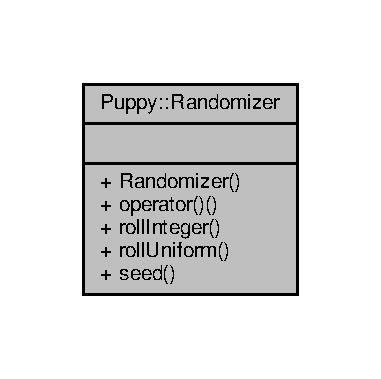
\includegraphics[width=183pt]{classPuppy_1_1Randomizer__coll__graph}
\end{center}
\end{figure}
\subsection*{Public Member Functions}
\begin{DoxyCompactItemize}
\item 
unsigned long \hyperlink{classPuppy_1_1Randomizer_a5eb79b633ba7cb009cce593a34dc8e27}{operator()} (unsigned long in\+N)
\begin{DoxyCompactList}\small\item\em Generate a randomly generated integer in range \mbox{[}0,in\+N). \end{DoxyCompactList}\item 
long \hyperlink{classPuppy_1_1Randomizer_ad1086e7ea63f1fd0cbf077001963a3bc}{roll\+Integer} (long in\+Low, long in\+Up)
\begin{DoxyCompactList}\small\item\em Generate a randomly generated integer in range \mbox{[}in\+Low,in\+Up\mbox{]}. \end{DoxyCompactList}\item 
double \hyperlink{classPuppy_1_1Randomizer_aa5dd7d1aa93080943275b0e56634f2ea}{roll\+Uniform} (double in\+Low=0.\+0, double in\+Up=1.\+0)
\begin{DoxyCompactList}\small\item\em Generate a uniformly generated random real number in range \mbox{[}in\+Low,in\+Up). \end{DoxyCompactList}\item 
void \hyperlink{classPuppy_1_1Randomizer_a46771ed34b2950edb092327db06bbe7f}{seed} (unsigned long in\+Seed=0)
\begin{DoxyCompactList}\small\item\em Initialize the random number generator. \end{DoxyCompactList}\end{DoxyCompactItemize}


\subsection{Detailed Description}
Random number generator. C++ wrapper over standard C rand and srand functions. 

\begin{DoxyParagraph}{Note\+:}
The operator() allow compliance with the S\+T\+L random number generator interface. 
\end{DoxyParagraph}


\subsection{Member Function Documentation}
\hypertarget{classPuppy_1_1Randomizer_a5eb79b633ba7cb009cce593a34dc8e27}{}\index{Puppy\+::\+Randomizer@{Puppy\+::\+Randomizer}!operator()@{operator()}}
\index{operator()@{operator()}!Puppy\+::\+Randomizer@{Puppy\+::\+Randomizer}}
\subsubsection[{operator()}]{\setlength{\rightskip}{0pt plus 5cm}unsigned long Puppy\+::\+Randomizer\+::operator() (
\begin{DoxyParamCaption}
\item[{unsigned long}]{in\+N}
\end{DoxyParamCaption}
)\hspace{0.3cm}{\ttfamily [inline]}}\label{classPuppy_1_1Randomizer_a5eb79b633ba7cb009cce593a34dc8e27}


Generate a randomly generated integer in range \mbox{[}0,in\+N). 

\begin{DoxyReturn}{Returns}
Randomly generated integer. 
\end{DoxyReturn}
\hypertarget{classPuppy_1_1Randomizer_ad1086e7ea63f1fd0cbf077001963a3bc}{}\index{Puppy\+::\+Randomizer@{Puppy\+::\+Randomizer}!roll\+Integer@{roll\+Integer}}
\index{roll\+Integer@{roll\+Integer}!Puppy\+::\+Randomizer@{Puppy\+::\+Randomizer}}
\subsubsection[{roll\+Integer}]{\setlength{\rightskip}{0pt plus 5cm}long Puppy\+::\+Randomizer\+::roll\+Integer (
\begin{DoxyParamCaption}
\item[{long}]{in\+Low, }
\item[{long}]{in\+Up}
\end{DoxyParamCaption}
)\hspace{0.3cm}{\ttfamily [inline]}}\label{classPuppy_1_1Randomizer_ad1086e7ea63f1fd0cbf077001963a3bc}


Generate a randomly generated integer in range \mbox{[}in\+Low,in\+Up\mbox{]}. 


\begin{DoxyParams}{Parameters}
{\em in\+Low} & Lower bound of generation range. \\
\hline
{\em in\+Up} & Upper bound of generation range. \\
\hline
\end{DoxyParams}
\begin{DoxyReturn}{Returns}
Randomly generated integer. 
\end{DoxyReturn}
\hypertarget{classPuppy_1_1Randomizer_aa5dd7d1aa93080943275b0e56634f2ea}{}\index{Puppy\+::\+Randomizer@{Puppy\+::\+Randomizer}!roll\+Uniform@{roll\+Uniform}}
\index{roll\+Uniform@{roll\+Uniform}!Puppy\+::\+Randomizer@{Puppy\+::\+Randomizer}}
\subsubsection[{roll\+Uniform}]{\setlength{\rightskip}{0pt plus 5cm}double Puppy\+::\+Randomizer\+::roll\+Uniform (
\begin{DoxyParamCaption}
\item[{double}]{in\+Low = {\ttfamily 0.0}, }
\item[{double}]{in\+Up = {\ttfamily 1.0}}
\end{DoxyParamCaption}
)\hspace{0.3cm}{\ttfamily [inline]}}\label{classPuppy_1_1Randomizer_aa5dd7d1aa93080943275b0e56634f2ea}


Generate a uniformly generated random real number in range \mbox{[}in\+Low,in\+Up). 


\begin{DoxyParams}{Parameters}
{\em in\+Low} & Lower bound of generation range. \\
\hline
{\em in\+Up} & Upper bound of generation range. \\
\hline
\end{DoxyParams}
\begin{DoxyReturn}{Returns}
Randomly generated real number. 
\end{DoxyReturn}
\hypertarget{classPuppy_1_1Randomizer_a46771ed34b2950edb092327db06bbe7f}{}\index{Puppy\+::\+Randomizer@{Puppy\+::\+Randomizer}!seed@{seed}}
\index{seed@{seed}!Puppy\+::\+Randomizer@{Puppy\+::\+Randomizer}}
\subsubsection[{seed}]{\setlength{\rightskip}{0pt plus 5cm}void Puppy\+::\+Randomizer\+::seed (
\begin{DoxyParamCaption}
\item[{unsigned long}]{in\+Seed = {\ttfamily 0}}
\end{DoxyParamCaption}
)\hspace{0.3cm}{\ttfamily [inline]}}\label{classPuppy_1_1Randomizer_a46771ed34b2950edb092327db06bbe7f}


Initialize the random number generator. 


\begin{DoxyParams}{Parameters}
{\em in\+Seed} & Seed to use. If zero, C\+P\+U clock value is used. \\
\hline
\end{DoxyParams}
\begin{DoxyReturn}{Returns}
Randomly generated integer. 
\end{DoxyReturn}


The documentation for this class was generated from the following file\+:\begin{DoxyCompactItemize}
\item 
source/puppy\+\_\+randomizer.\+hpp\end{DoxyCompactItemize}

\hypertarget{classRosenbrock}{}\section{Rosenbrock Class Reference}
\label{classRosenbrock}\index{Rosenbrock@{Rosenbrock}}


Inheritance diagram for Rosenbrock\+:
\nopagebreak
\begin{figure}[H]
\begin{center}
\leavevmode
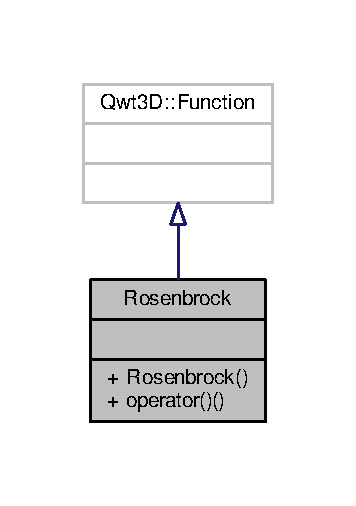
\includegraphics[width=171pt]{classRosenbrock__inherit__graph}
\end{center}
\end{figure}


Collaboration diagram for Rosenbrock\+:
\nopagebreak
\begin{figure}[H]
\begin{center}
\leavevmode
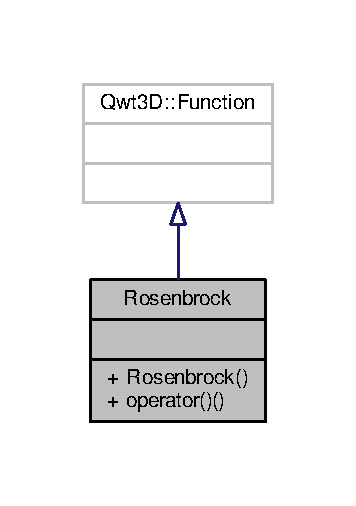
\includegraphics[width=171pt]{classRosenbrock__coll__graph}
\end{center}
\end{figure}
\subsection*{Public Member Functions}
\begin{DoxyCompactItemize}
\item 
\hypertarget{classRosenbrock_aa8803fd4e38a835de1d7b71299e2b11b}{}{\bfseries Rosenbrock} (Qwt3\+D\+::\+Grid\+Plot \&pw)\label{classRosenbrock_aa8803fd4e38a835de1d7b71299e2b11b}

\item 
\hypertarget{classRosenbrock_ab583f473d97114aad858d383f4fbc9b1}{}double {\bfseries operator()} (double x, double y)\label{classRosenbrock_ab583f473d97114aad858d383f4fbc9b1}

\end{DoxyCompactItemize}


The documentation for this class was generated from the following file\+:\begin{DoxyCompactItemize}
\item 
source/mainwindow.\+cpp\end{DoxyCompactItemize}

\hypertarget{classSin}{}\section{Sin Class Reference}
\label{classSin}\index{Sin@{Sin}}


Inheritance diagram for Sin\+:
\nopagebreak
\begin{figure}[H]
\begin{center}
\leavevmode
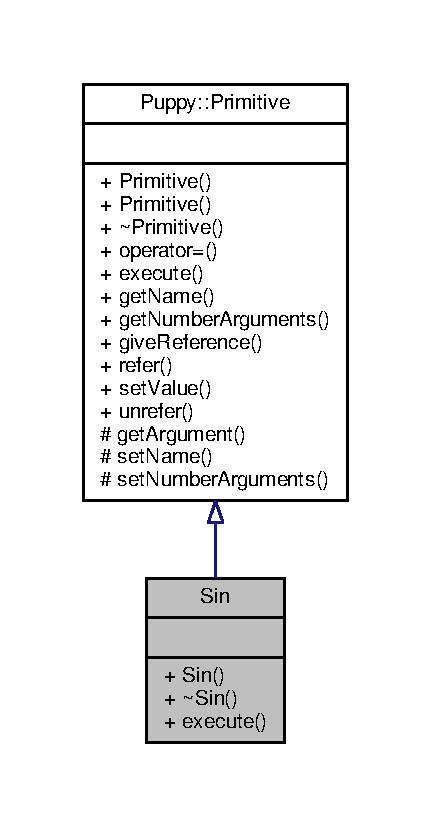
\includegraphics[width=207pt]{classSin__inherit__graph}
\end{center}
\end{figure}


Collaboration diagram for Sin\+:
\nopagebreak
\begin{figure}[H]
\begin{center}
\leavevmode
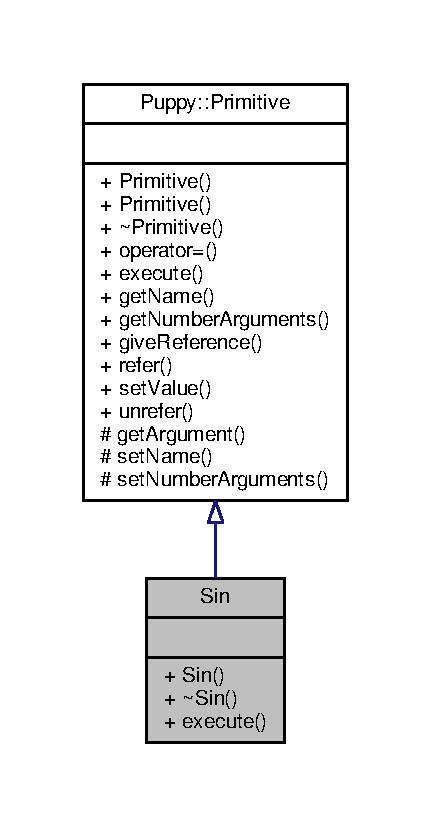
\includegraphics[width=207pt]{classSin__coll__graph}
\end{center}
\end{figure}
\subsection*{Public Member Functions}
\begin{DoxyCompactItemize}
\item 
\hypertarget{classSin_ae1f86757154337ee08d5c08033bc2b31}{}\hyperlink{classSin_ae1f86757154337ee08d5c08033bc2b31}{Sin} ()\label{classSin_ae1f86757154337ee08d5c08033bc2b31}

\begin{DoxyCompactList}\small\item\em Construct \hyperlink{classSin}{Sin} G\+P primitive. \end{DoxyCompactList}\item 
virtual void \hyperlink{classSin_a52e8e8096eb90f30418dc74e0a89a1ec}{execute} (void $\ast$out\+Datum, \hyperlink{classPuppy_1_1Context}{Puppy\+::\+Context} \&io\+Context)
\begin{DoxyCompactList}\small\item\em Execute characteristic operation of \hyperlink{classSin}{Sin} primitive. \end{DoxyCompactList}\end{DoxyCompactItemize}
\subsection*{Additional Inherited Members}


\subsection{Member Function Documentation}
\hypertarget{classSin_a52e8e8096eb90f30418dc74e0a89a1ec}{}\index{Sin@{Sin}!execute@{execute}}
\index{execute@{execute}!Sin@{Sin}}
\subsubsection[{execute}]{\setlength{\rightskip}{0pt plus 5cm}void Sin\+::execute (
\begin{DoxyParamCaption}
\item[{void $\ast$}]{out\+Datum, }
\item[{{\bf Puppy\+::\+Context} \&}]{io\+Context}
\end{DoxyParamCaption}
)\hspace{0.3cm}{\ttfamily [virtual]}}\label{classSin_a52e8e8096eb90f30418dc74e0a89a1ec}


Execute characteristic operation of \hyperlink{classSin}{Sin} primitive. 


\begin{DoxyParams}{Parameters}
{\em out\+Datum} & Result of the \hyperlink{classSin}{Sin} operation. \\
\hline
{\em io\+Context} & Evolutionary context. \\
\hline
\end{DoxyParams}


Implements \hyperlink{classPuppy_1_1Primitive_aaef85034e66f49903c591158c3b5ffef}{Puppy\+::\+Primitive}.



The documentation for this class was generated from the following files\+:\begin{DoxyCompactItemize}
\item 
source/puppy\+\_\+regprimitives.\+hpp\item 
source/puppy\+\_\+regprimitives.\+cpp\end{DoxyCompactItemize}

\hypertarget{structWorker_1_1Stats}{}\section{Worker\+:\+:Stats Struct Reference}
\label{structWorker_1_1Stats}\index{Worker\+::\+Stats@{Worker\+::\+Stats}}


Collaboration diagram for Worker\+:\+:Stats\+:
\nopagebreak
\begin{figure}[H]
\begin{center}
\leavevmode
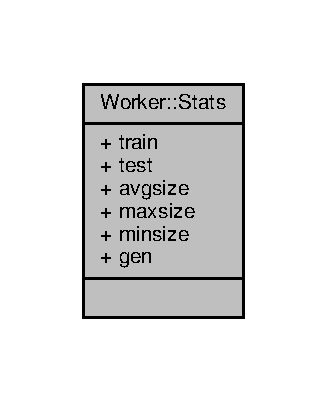
\includegraphics[width=157pt]{structWorker_1_1Stats__coll__graph}
\end{center}
\end{figure}
\subsection*{Public Attributes}
\begin{DoxyCompactItemize}
\item 
\hypertarget{structWorker_1_1Stats_afa4ac31dd6f66421c766e24b8ea31021}{}double {\bfseries train}\label{structWorker_1_1Stats_afa4ac31dd6f66421c766e24b8ea31021}

\item 
\hypertarget{structWorker_1_1Stats_a9d0473d4ac1c37896cdf99e431ba9564}{}double {\bfseries test}\label{structWorker_1_1Stats_a9d0473d4ac1c37896cdf99e431ba9564}

\item 
\hypertarget{structWorker_1_1Stats_a77911ac9d1453454291186928a775ac7}{}double {\bfseries avgsize}\label{structWorker_1_1Stats_a77911ac9d1453454291186928a775ac7}

\item 
\hypertarget{structWorker_1_1Stats_a205caf72b0bfde3224de9e464546606e}{}double {\bfseries maxsize}\label{structWorker_1_1Stats_a205caf72b0bfde3224de9e464546606e}

\item 
\hypertarget{structWorker_1_1Stats_a20c63fe5e2fee97b0ae04dcfd4cc29ad}{}double {\bfseries minsize}\label{structWorker_1_1Stats_a20c63fe5e2fee97b0ae04dcfd4cc29ad}

\item 
\hypertarget{structWorker_1_1Stats_a4d79155d9f6534c939e73662cdb714ed}{}double {\bfseries gen}\label{structWorker_1_1Stats_a4d79155d9f6534c939e73662cdb714ed}

\end{DoxyCompactItemize}


The documentation for this struct was generated from the following file\+:\begin{DoxyCompactItemize}
\item 
source/worker.\+h\end{DoxyCompactItemize}

\hypertarget{classSubtract}{}\section{Subtract Class Reference}
\label{classSubtract}\index{Subtract@{Subtract}}


\hyperlink{classSubtract}{Subtract} two doubles G\+P primitive.  




Inheritance diagram for Subtract\+:
\nopagebreak
\begin{figure}[H]
\begin{center}
\leavevmode
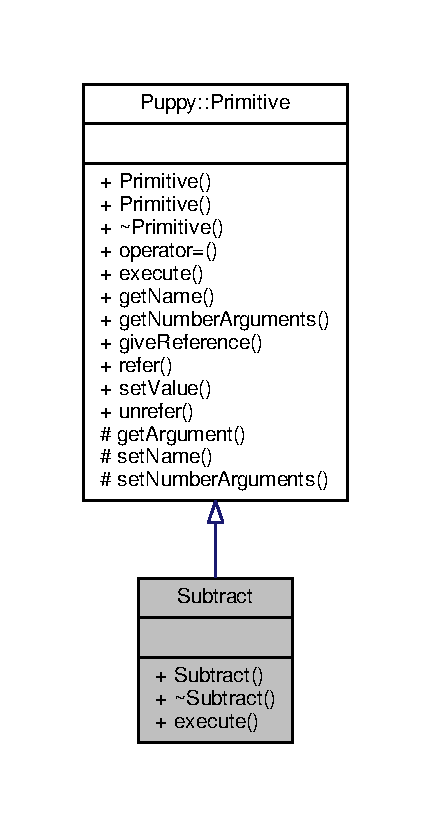
\includegraphics[width=207pt]{classSubtract__inherit__graph}
\end{center}
\end{figure}


Collaboration diagram for Subtract\+:
\nopagebreak
\begin{figure}[H]
\begin{center}
\leavevmode
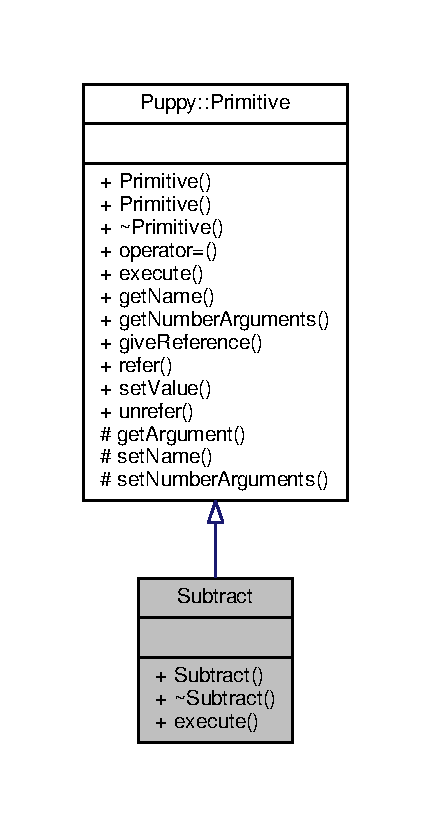
\includegraphics[width=207pt]{classSubtract__coll__graph}
\end{center}
\end{figure}
\subsection*{Public Member Functions}
\begin{DoxyCompactItemize}
\item 
\hypertarget{classSubtract_a00e1bfb4f3eb6f166abef10490ccba3b}{}\hyperlink{classSubtract_a00e1bfb4f3eb6f166abef10490ccba3b}{Subtract} ()\label{classSubtract_a00e1bfb4f3eb6f166abef10490ccba3b}

\begin{DoxyCompactList}\small\item\em Construct \hyperlink{classSubtract}{Subtract} G\+P primitive. \end{DoxyCompactList}\item 
virtual void \hyperlink{classSubtract_a7b85b95cd90fe9633ba684802343d2e2}{execute} (void $\ast$out\+Datum, \hyperlink{classPuppy_1_1Context}{Puppy\+::\+Context} \&io\+Context)
\begin{DoxyCompactList}\small\item\em Execute characteristic operation of \hyperlink{classSubtract}{Subtract} primitive. \end{DoxyCompactList}\end{DoxyCompactItemize}
\subsection*{Additional Inherited Members}


\subsection{Detailed Description}
\hyperlink{classSubtract}{Subtract} two doubles G\+P primitive. 

\subsection{Member Function Documentation}
\hypertarget{classSubtract_a7b85b95cd90fe9633ba684802343d2e2}{}\index{Subtract@{Subtract}!execute@{execute}}
\index{execute@{execute}!Subtract@{Subtract}}
\subsubsection[{execute}]{\setlength{\rightskip}{0pt plus 5cm}void Subtract\+::execute (
\begin{DoxyParamCaption}
\item[{void $\ast$}]{out\+Datum, }
\item[{{\bf Puppy\+::\+Context} \&}]{io\+Context}
\end{DoxyParamCaption}
)\hspace{0.3cm}{\ttfamily [virtual]}}\label{classSubtract_a7b85b95cd90fe9633ba684802343d2e2}


Execute characteristic operation of \hyperlink{classSubtract}{Subtract} primitive. 


\begin{DoxyParams}{Parameters}
{\em out\+Datum} & Result of the \hyperlink{classSubtract}{Subtract} operation. \\
\hline
{\em io\+Context} & Evolutionary context. \\
\hline
\end{DoxyParams}


Implements \hyperlink{classPuppy_1_1Primitive_aaef85034e66f49903c591158c3b5ffef}{Puppy\+::\+Primitive}.



The documentation for this class was generated from the following files\+:\begin{DoxyCompactItemize}
\item 
source/puppy\+\_\+regprimitives.\+hpp\item 
source/puppy\+\_\+regprimitives.\+cpp\end{DoxyCompactItemize}

\hypertarget{classPuppy_1_1TokenT}{}\section{Puppy\+:\+:Token\+T$<$ T $>$ Class Template Reference}
\label{classPuppy_1_1TokenT}\index{Puppy\+::\+Token\+T$<$ T $>$@{Puppy\+::\+Token\+T$<$ T $>$}}


Token template, to use as variable terminal primitive.  




Inheritance diagram for Puppy\+:\+:Token\+T$<$ T $>$\+:
\nopagebreak
\begin{figure}[H]
\begin{center}
\leavevmode
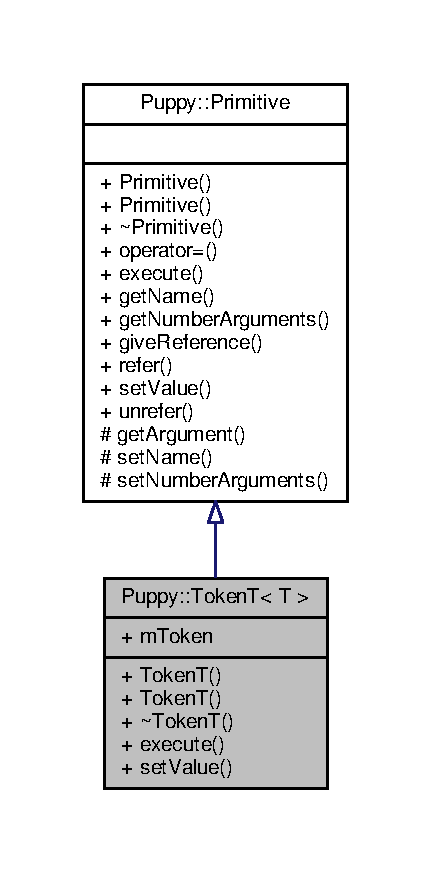
\includegraphics[width=207pt]{classPuppy_1_1TokenT__inherit__graph}
\end{center}
\end{figure}


Collaboration diagram for Puppy\+:\+:Token\+T$<$ T $>$\+:
\nopagebreak
\begin{figure}[H]
\begin{center}
\leavevmode
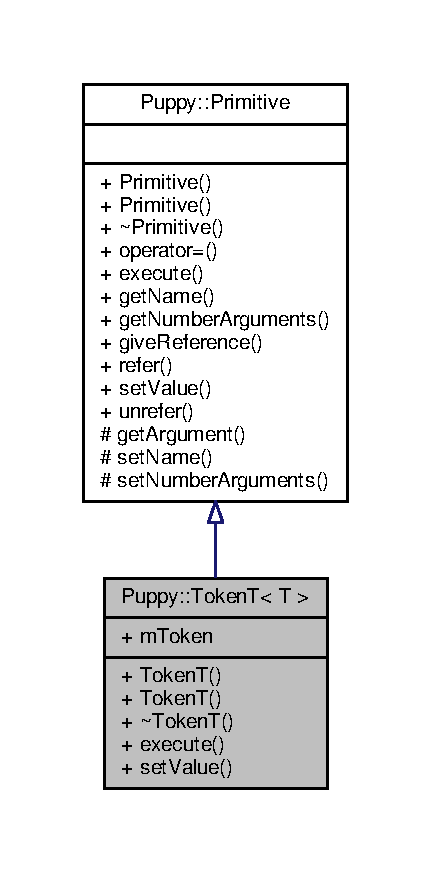
\includegraphics[width=207pt]{classPuppy_1_1TokenT__coll__graph}
\end{center}
\end{figure}
\subsection*{Public Member Functions}
\begin{DoxyCompactItemize}
\item 
\hyperlink{classPuppy_1_1TokenT_a6a7b7bfc007d988e971e27bd1dec45ef}{Token\+T} (std\+::string in\+Name=\char`\"{}T\+O\+K\+E\+N\char`\"{})
\begin{DoxyCompactList}\small\item\em Construct a token primitive. \end{DoxyCompactList}\item 
\hyperlink{classPuppy_1_1TokenT_a459a16b36d08f3d4fddd41f720bdd7e2}{Token\+T} (std\+::string in\+Name, const T \&in\+Token)
\begin{DoxyCompactList}\small\item\em Construct a token primitive. \end{DoxyCompactList}\item 
virtual void \hyperlink{classPuppy_1_1TokenT_a15641f373da2d98c057247c32deb943a}{execute} (void $\ast$out\+Datum, \hyperlink{classPuppy_1_1Context}{Context} \&io\+Context)
\begin{DoxyCompactList}\small\item\em Execute the caracteristic token primitive operation. \end{DoxyCompactList}\item 
virtual void \hyperlink{classPuppy_1_1TokenT_ad38ced7ce46e1ef1449bd90560296f3f}{set\+Value} (const void $\ast$in\+Value)
\begin{DoxyCompactList}\small\item\em Set the value of the token primitive. \end{DoxyCompactList}\end{DoxyCompactItemize}
\subsection*{Public Attributes}
\begin{DoxyCompactItemize}
\item 
\hypertarget{classPuppy_1_1TokenT_abb63e082387b0aa4f8986ae52f020020}{}T \hyperlink{classPuppy_1_1TokenT_abb63e082387b0aa4f8986ae52f020020}{m\+Token}\label{classPuppy_1_1TokenT_abb63e082387b0aa4f8986ae52f020020}

\begin{DoxyCompactList}\small\item\em Token value of the primitive. \end{DoxyCompactList}\end{DoxyCompactItemize}
\subsection*{Additional Inherited Members}


\subsection{Detailed Description}
\subsubsection*{template$<$class T$>$class Puppy\+::\+Token\+T$<$ T $>$}

Token template, to use as variable terminal primitive. 


\begin{DoxyParams}{Parameters}
{\em T} & Templated type. \\
\hline
\end{DoxyParams}


\subsection{Constructor \& Destructor Documentation}
\hypertarget{classPuppy_1_1TokenT_a6a7b7bfc007d988e971e27bd1dec45ef}{}\index{Puppy\+::\+Token\+T@{Puppy\+::\+Token\+T}!Token\+T@{Token\+T}}
\index{Token\+T@{Token\+T}!Puppy\+::\+Token\+T@{Puppy\+::\+Token\+T}}
\subsubsection[{Token\+T}]{\setlength{\rightskip}{0pt plus 5cm}template$<$class T $>$ {\bf Puppy\+::\+Token\+T}$<$ T $>$\+::{\bf Token\+T} (
\begin{DoxyParamCaption}
\item[{std\+::string}]{in\+Name = {\ttfamily \char`\"{}TOKEN\char`\"{}}}
\end{DoxyParamCaption}
)\hspace{0.3cm}{\ttfamily [explicit]}}\label{classPuppy_1_1TokenT_a6a7b7bfc007d988e971e27bd1dec45ef}


Construct a token primitive. 


\begin{DoxyParams}{Parameters}
{\em in\+Name} & Name of the primitive. \\
\hline
\end{DoxyParams}
\hypertarget{classPuppy_1_1TokenT_a459a16b36d08f3d4fddd41f720bdd7e2}{}\index{Puppy\+::\+Token\+T@{Puppy\+::\+Token\+T}!Token\+T@{Token\+T}}
\index{Token\+T@{Token\+T}!Puppy\+::\+Token\+T@{Puppy\+::\+Token\+T}}
\subsubsection[{Token\+T}]{\setlength{\rightskip}{0pt plus 5cm}template$<$class T $>$ {\bf Puppy\+::\+Token\+T}$<$ T $>$\+::{\bf Token\+T} (
\begin{DoxyParamCaption}
\item[{std\+::string}]{in\+Name, }
\item[{const T \&}]{in\+Token}
\end{DoxyParamCaption}
)\hspace{0.3cm}{\ttfamily [explicit]}}\label{classPuppy_1_1TokenT_a459a16b36d08f3d4fddd41f720bdd7e2}


Construct a token primitive. 


\begin{DoxyParams}{Parameters}
{\em in\+Name} & Name of the primitive. \\
\hline
{\em in\+Token} & Value of the token. \\
\hline
\end{DoxyParams}


\subsection{Member Function Documentation}
\hypertarget{classPuppy_1_1TokenT_a15641f373da2d98c057247c32deb943a}{}\index{Puppy\+::\+Token\+T@{Puppy\+::\+Token\+T}!execute@{execute}}
\index{execute@{execute}!Puppy\+::\+Token\+T@{Puppy\+::\+Token\+T}}
\subsubsection[{execute}]{\setlength{\rightskip}{0pt plus 5cm}template$<$class T $>$ void {\bf Puppy\+::\+Token\+T}$<$ T $>$\+::execute (
\begin{DoxyParamCaption}
\item[{void $\ast$}]{out\+Datum, }
\item[{{\bf Puppy\+::\+Context} \&}]{io\+Context}
\end{DoxyParamCaption}
)\hspace{0.3cm}{\ttfamily [virtual]}}\label{classPuppy_1_1TokenT_a15641f373da2d98c057247c32deb943a}


Execute the caracteristic token primitive operation. 


\begin{DoxyParams}{Parameters}
{\em out\+Datum} & Result of the execution. \\
\hline
{\em io\+Context} & Evolutionary context. \\
\hline
\end{DoxyParams}


Implements \hyperlink{classPuppy_1_1Primitive_aaef85034e66f49903c591158c3b5ffef}{Puppy\+::\+Primitive}.

\hypertarget{classPuppy_1_1TokenT_ad38ced7ce46e1ef1449bd90560296f3f}{}\index{Puppy\+::\+Token\+T@{Puppy\+::\+Token\+T}!set\+Value@{set\+Value}}
\index{set\+Value@{set\+Value}!Puppy\+::\+Token\+T@{Puppy\+::\+Token\+T}}
\subsubsection[{set\+Value}]{\setlength{\rightskip}{0pt plus 5cm}template$<$class T $>$ void {\bf Puppy\+::\+Token\+T}$<$ T $>$\+::set\+Value (
\begin{DoxyParamCaption}
\item[{const void $\ast$}]{in\+Value}
\end{DoxyParamCaption}
)\hspace{0.3cm}{\ttfamily [virtual]}}\label{classPuppy_1_1TokenT_ad38ced7ce46e1ef1449bd90560296f3f}


Set the value of the token primitive. 


\begin{DoxyParams}{Parameters}
{\em in\+Value} & Value of the token. \\
\hline
\end{DoxyParams}


Reimplemented from \hyperlink{classPuppy_1_1Primitive_a2cd429caecd22c31166230b3467fb861}{Puppy\+::\+Primitive}.



The documentation for this class was generated from the following file\+:\begin{DoxyCompactItemize}
\item 
source/puppy\+\_\+token\+T.\+hpp\end{DoxyCompactItemize}

\hypertarget{classPuppy_1_1Tree}{}\section{Puppy\+:\+:Tree Class Reference}
\label{classPuppy_1_1Tree}\index{Puppy\+::\+Tree@{Puppy\+::\+Tree}}


G\+P tree class.

The evolutionary context includes the execution context used when interpreting the trees along with the problem set-\/up defined with the function and terminal set, and the randomizer.  




Inheritance diagram for Puppy\+:\+:Tree\+:
\nopagebreak
\begin{figure}[H]
\begin{center}
\leavevmode
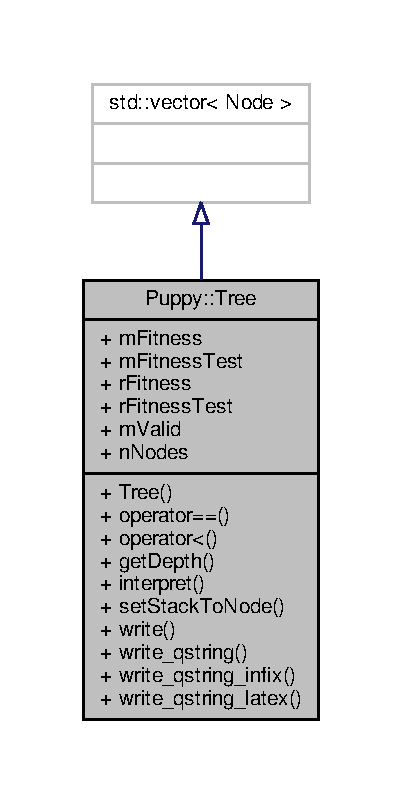
\includegraphics[width=193pt]{classPuppy_1_1Tree__inherit__graph}
\end{center}
\end{figure}


Collaboration diagram for Puppy\+:\+:Tree\+:
\nopagebreak
\begin{figure}[H]
\begin{center}
\leavevmode
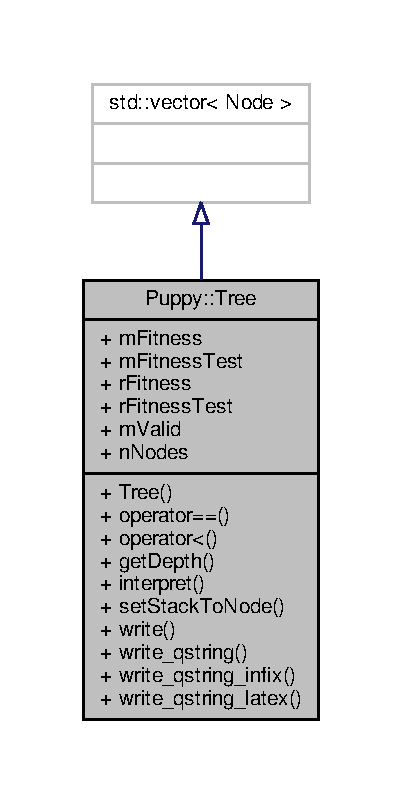
\includegraphics[width=193pt]{classPuppy_1_1Tree__coll__graph}
\end{center}
\end{figure}
\subsection*{Public Member Functions}
\begin{DoxyCompactItemize}
\item 
\hyperlink{classPuppy_1_1Tree_ac3a0b230da2e70ecbd801dc1508a3663}{Tree} (float in\+Fitness=-\/1.\+0, bool in\+Valid=false)
\begin{DoxyCompactList}\small\item\em Construct a new tree, with given fitness and validity flag. \end{DoxyCompactList}\item 
bool \hyperlink{classPuppy_1_1Tree_a51989208ace756d41a16e8eb35d03cb5}{operator==} (const \hyperlink{classPuppy_1_1Tree}{Tree} \&in\+Right\+Tree) const 
\begin{DoxyCompactList}\small\item\em Compare equality of two trees. \end{DoxyCompactList}\item 
bool \hyperlink{classPuppy_1_1Tree_a60a5ef4dc1298a93810f065a5fffc906}{operator$<$} (const \hyperlink{classPuppy_1_1Tree}{Tree} \&in\+Right\+Tree) const 
\begin{DoxyCompactList}\small\item\em Compare ranking of two trees. \end{DoxyCompactList}\item 
unsigned int \hyperlink{classPuppy_1_1Tree_aa5979533de55c89eb808a69288db5a1b}{get\+Depth} (unsigned int in\+Index=0) const 
\begin{DoxyCompactList}\small\item\em Return tree depth at given index. \end{DoxyCompactList}\item 
void \hyperlink{classPuppy_1_1Tree_aa9e48062cd1ee1d9c8dca83686f35fb1}{interpret} (void $\ast$out\+Result, \hyperlink{classPuppy_1_1Context}{Context} \&io\+Context)
\begin{DoxyCompactList}\small\item\em Interpret the G\+P tree. \end{DoxyCompactList}\item 
void \hyperlink{classPuppy_1_1Tree_a23ae7305ae065dfccf354b3d4ba306c7}{set\+Stack\+To\+Node} (unsigned int in\+Index, std\+::vector$<$ unsigned int $>$ \&out\+Call\+Stack) const 
\begin{DoxyCompactList}\small\item\em Set call stack to include the correctly refer to a given node. \end{DoxyCompactList}\item 
void \hyperlink{classPuppy_1_1Tree_ae7cf5b8e64273dc265a2e751f4a06ffb}{write} (std\+::ostream \&io\+O\+S, unsigned int in\+Index=0) const 
\begin{DoxyCompactList}\small\item\em Write G\+P tree at given index as a s-\/expression into a C++ output stream. \end{DoxyCompactList}\item 
\hypertarget{classPuppy_1_1Tree_a7b051f1143713fb9dc754abaa995fa05}{}void {\bfseries write\+\_\+qstring} (Q\+String \&io\+O\+S, unsigned int in\+Index=0) const \label{classPuppy_1_1Tree_a7b051f1143713fb9dc754abaa995fa05}

\item 
\hypertarget{classPuppy_1_1Tree_a0efdb3778f18a4aec63d9482aeb7ad55}{}void {\bfseries write\+\_\+qstring\+\_\+infix} (Q\+String \&io\+O\+S, unsigned int in\+Index=0) const \label{classPuppy_1_1Tree_a0efdb3778f18a4aec63d9482aeb7ad55}

\item 
\hypertarget{classPuppy_1_1Tree_aa464eae9cf144f8525320f23d00a8172}{}void {\bfseries write\+\_\+qstring\+\_\+latex} (Q\+String \&io\+O\+S, unsigned int in\+Index=0) const \label{classPuppy_1_1Tree_aa464eae9cf144f8525320f23d00a8172}

\end{DoxyCompactItemize}
\subsection*{Public Attributes}
\begin{DoxyCompactItemize}
\item 
\hypertarget{classPuppy_1_1Tree_a570b092e1827472f39dba11df2bfdbca}{}float \hyperlink{classPuppy_1_1Tree_a570b092e1827472f39dba11df2bfdbca}{m\+Fitness}\label{classPuppy_1_1Tree_a570b092e1827472f39dba11df2bfdbca}

\begin{DoxyCompactList}\small\item\em Fitness value of the G\+P tree. \end{DoxyCompactList}\item 
\hypertarget{classPuppy_1_1Tree_ad110a4c393135da8fd0eb603ac671f10}{}float {\bfseries m\+Fitness\+Test}\label{classPuppy_1_1Tree_ad110a4c393135da8fd0eb603ac671f10}

\item 
\hypertarget{classPuppy_1_1Tree_aafd16788f30f4f5474e19899edc848e4}{}float {\bfseries r\+Fitness}\label{classPuppy_1_1Tree_aafd16788f30f4f5474e19899edc848e4}

\item 
\hypertarget{classPuppy_1_1Tree_a3f8ddcf28b4ea6b1461839d131244b00}{}float {\bfseries r\+Fitness\+Test}\label{classPuppy_1_1Tree_a3f8ddcf28b4ea6b1461839d131244b00}

\item 
\hypertarget{classPuppy_1_1Tree_a3acb505d5915892a986b4a5ee0eb1e87}{}bool \hyperlink{classPuppy_1_1Tree_a3acb505d5915892a986b4a5ee0eb1e87}{m\+Valid}\label{classPuppy_1_1Tree_a3acb505d5915892a986b4a5ee0eb1e87}

\begin{DoxyCompactList}\small\item\em Flag indicating whether the fitness is valid. \end{DoxyCompactList}\item 
\hypertarget{classPuppy_1_1Tree_a31d5ff402f9d01fbd4043507e4abd8c9}{}int {\bfseries n\+Nodes}\label{classPuppy_1_1Tree_a31d5ff402f9d01fbd4043507e4abd8c9}

\end{DoxyCompactItemize}
\subsection*{Related Functions}
(Note that these are not member functions.) \begin{DoxyCompactItemize}
\item 
std\+::ostream \& \hyperlink{group__Puppy_ga055f36ab366f6ac84c28e0f7f19103e2}{operator$<$$<$} (std\+::ostream \&io\+O\+S, const \hyperlink{classPuppy_1_1Tree}{Puppy\+::\+Tree} \&in\+Tree)
\begin{DoxyCompactList}\small\item\em Write tree into output stream with function \hyperlink{classPuppy_1_1Tree_ae7cf5b8e64273dc265a2e751f4a06ffb}{Puppy\+::\+Tree\+::write}. \end{DoxyCompactList}\end{DoxyCompactItemize}


\subsection{Detailed Description}
G\+P tree class.

The evolutionary context includes the execution context used when interpreting the trees along with the problem set-\/up defined with the function and terminal set, and the randomizer. 

\subsection{Constructor \& Destructor Documentation}
\hypertarget{classPuppy_1_1Tree_ac3a0b230da2e70ecbd801dc1508a3663}{}\index{Puppy\+::\+Tree@{Puppy\+::\+Tree}!Tree@{Tree}}
\index{Tree@{Tree}!Puppy\+::\+Tree@{Puppy\+::\+Tree}}
\subsubsection[{Tree}]{\setlength{\rightskip}{0pt plus 5cm}Puppy\+::\+Tree\+::\+Tree (
\begin{DoxyParamCaption}
\item[{float}]{in\+Fitness = {\ttfamily -\/1.0}, }
\item[{bool}]{in\+Valid = {\ttfamily false}}
\end{DoxyParamCaption}
)\hspace{0.3cm}{\ttfamily [explicit]}}\label{classPuppy_1_1Tree_ac3a0b230da2e70ecbd801dc1508a3663}


Construct a new tree, with given fitness and validity flag. 


\begin{DoxyParams}{Parameters}
{\em in\+Fitness} & Fitness value of the G\+P tree. \\
\hline
{\em in\+Valid} & Validity of the fitness value. \\
\hline
\end{DoxyParams}


\subsection{Member Function Documentation}
\hypertarget{classPuppy_1_1Tree_aa5979533de55c89eb808a69288db5a1b}{}\index{Puppy\+::\+Tree@{Puppy\+::\+Tree}!get\+Depth@{get\+Depth}}
\index{get\+Depth@{get\+Depth}!Puppy\+::\+Tree@{Puppy\+::\+Tree}}
\subsubsection[{get\+Depth}]{\setlength{\rightskip}{0pt plus 5cm}unsigned int Puppy\+::\+Tree\+::get\+Depth (
\begin{DoxyParamCaption}
\item[{unsigned int}]{in\+Index = {\ttfamily 0}}
\end{DoxyParamCaption}
) const}\label{classPuppy_1_1Tree_aa5979533de55c89eb808a69288db5a1b}


Return tree depth at given index. 


\begin{DoxyParams}{Parameters}
{\em in\+Index} & Index of sub-\/tree root to get the depth from. \\
\hline
\end{DoxyParams}
\begin{DoxyReturn}{Returns}
Sub-\/tree depth. 
\end{DoxyReturn}
\hypertarget{classPuppy_1_1Tree_aa9e48062cd1ee1d9c8dca83686f35fb1}{}\index{Puppy\+::\+Tree@{Puppy\+::\+Tree}!interpret@{interpret}}
\index{interpret@{interpret}!Puppy\+::\+Tree@{Puppy\+::\+Tree}}
\subsubsection[{interpret}]{\setlength{\rightskip}{0pt plus 5cm}void Puppy\+::\+Tree\+::interpret (
\begin{DoxyParamCaption}
\item[{void $\ast$}]{out\+Result, }
\item[{{\bf Puppy\+::\+Context} \&}]{io\+Context}
\end{DoxyParamCaption}
)}\label{classPuppy_1_1Tree_aa9e48062cd1ee1d9c8dca83686f35fb1}


Interpret the G\+P tree. 


\begin{DoxyParams}{Parameters}
{\em out\+Result} & Datum containing the result of the interpretation. \\
\hline
{\em io\+Context} & Evolutionary context. \\
\hline
\end{DoxyParams}
\hypertarget{classPuppy_1_1Tree_a60a5ef4dc1298a93810f065a5fffc906}{}\index{Puppy\+::\+Tree@{Puppy\+::\+Tree}!operator$<$@{operator$<$}}
\index{operator$<$@{operator$<$}!Puppy\+::\+Tree@{Puppy\+::\+Tree}}
\subsubsection[{operator$<$}]{\setlength{\rightskip}{0pt plus 5cm}bool Puppy\+::\+Tree\+::operator$<$ (
\begin{DoxyParamCaption}
\item[{const {\bf Tree} \&}]{in\+Right\+Tree}
\end{DoxyParamCaption}
) const\hspace{0.3cm}{\ttfamily [inline]}}\label{classPuppy_1_1Tree_a60a5ef4dc1298a93810f065a5fffc906}


Compare ranking of two trees. 


\begin{DoxyParams}{Parameters}
{\em in\+Right\+Tree} & Second tree to compare to the actual. \\
\hline
\end{DoxyParams}
\begin{DoxyReturn}{Returns}
True is actual tree is less than seconf, false if not. 
\end{DoxyReturn}
\hypertarget{classPuppy_1_1Tree_a51989208ace756d41a16e8eb35d03cb5}{}\index{Puppy\+::\+Tree@{Puppy\+::\+Tree}!operator==@{operator==}}
\index{operator==@{operator==}!Puppy\+::\+Tree@{Puppy\+::\+Tree}}
\subsubsection[{operator==}]{\setlength{\rightskip}{0pt plus 5cm}bool Puppy\+::\+Tree\+::operator== (
\begin{DoxyParamCaption}
\item[{const {\bf Tree} \&}]{in\+Right\+Tree}
\end{DoxyParamCaption}
) const\hspace{0.3cm}{\ttfamily [inline]}}\label{classPuppy_1_1Tree_a51989208ace756d41a16e8eb35d03cb5}


Compare equality of two trees. 


\begin{DoxyParams}{Parameters}
{\em in\+Right\+Tree} & Second tree to compare to the actual. \\
\hline
\end{DoxyParams}
\begin{DoxyReturn}{Returns}
True is trees are equals, false if not. 
\end{DoxyReturn}
\hypertarget{classPuppy_1_1Tree_a23ae7305ae065dfccf354b3d4ba306c7}{}\index{Puppy\+::\+Tree@{Puppy\+::\+Tree}!set\+Stack\+To\+Node@{set\+Stack\+To\+Node}}
\index{set\+Stack\+To\+Node@{set\+Stack\+To\+Node}!Puppy\+::\+Tree@{Puppy\+::\+Tree}}
\subsubsection[{set\+Stack\+To\+Node}]{\setlength{\rightskip}{0pt plus 5cm}void Puppy\+::\+Tree\+::set\+Stack\+To\+Node (
\begin{DoxyParamCaption}
\item[{unsigned int}]{in\+Index, }
\item[{std\+::vector$<$ unsigned int $>$ \&}]{out\+Call\+Stack}
\end{DoxyParamCaption}
) const}\label{classPuppy_1_1Tree_a23ae7305ae065dfccf354b3d4ba306c7}


Set call stack to include the correctly refer to a given node. 


\begin{DoxyParams}{Parameters}
{\em in\+Index} & \hyperlink{structPuppy_1_1Node}{Node} index to which call stack must be set. \\
\hline
{\em out\+Call\+Stack} & Result of call stack setting. \\
\hline
\end{DoxyParams}
\hypertarget{classPuppy_1_1Tree_ae7cf5b8e64273dc265a2e751f4a06ffb}{}\index{Puppy\+::\+Tree@{Puppy\+::\+Tree}!write@{write}}
\index{write@{write}!Puppy\+::\+Tree@{Puppy\+::\+Tree}}
\subsubsection[{write}]{\setlength{\rightskip}{0pt plus 5cm}void Puppy\+::\+Tree\+::write (
\begin{DoxyParamCaption}
\item[{std\+::ostream \&}]{io\+O\+S, }
\item[{unsigned int}]{in\+Index = {\ttfamily 0}}
\end{DoxyParamCaption}
) const}\label{classPuppy_1_1Tree_ae7cf5b8e64273dc265a2e751f4a06ffb}


Write G\+P tree at given index as a s-\/expression into a C++ output stream. 


\begin{DoxyParams}{Parameters}
{\em io\+O\+S} & C++ output stream to write tree into. \\
\hline
{\em in\+Index} & Actual node index in tree. \\
\hline
\end{DoxyParams}


The documentation for this class was generated from the following files\+:\begin{DoxyCompactItemize}
\item 
source/puppy\+\_\+tree.\+hpp\item 
source/puppy\+\_\+tree.\+cpp\end{DoxyCompactItemize}

\hypertarget{structWorker_1_1TreeContainer}{}\section{Worker\+:\+:Tree\+Container Struct Reference}
\label{structWorker_1_1TreeContainer}\index{Worker\+::\+Tree\+Container@{Worker\+::\+Tree\+Container}}


Collaboration diagram for Worker\+:\+:Tree\+Container\+:
\nopagebreak
\begin{figure}[H]
\begin{center}
\leavevmode
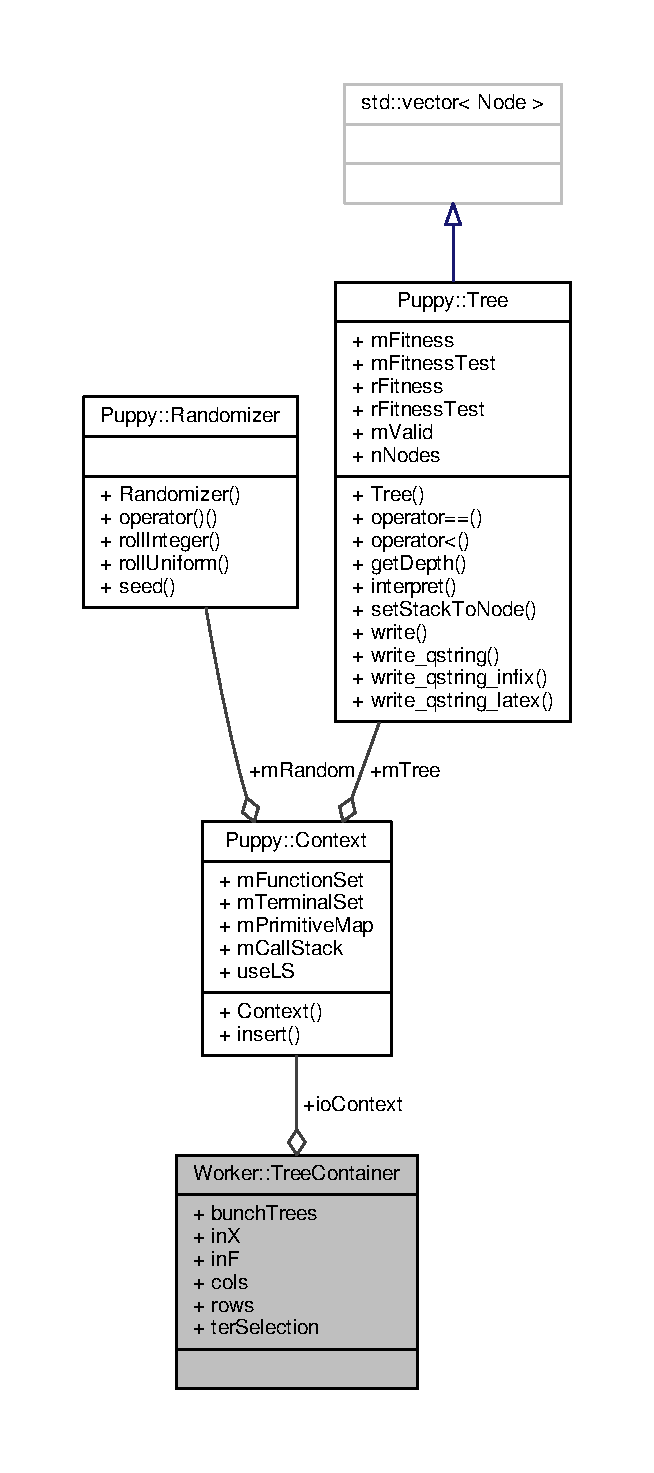
\includegraphics[height=550pt]{structWorker_1_1TreeContainer__coll__graph}
\end{center}
\end{figure}
\subsection*{Public Attributes}
\begin{DoxyCompactItemize}
\item 
\hypertarget{structWorker_1_1TreeContainer_a591e097ef7fa6a9418d027830ca7860e}{}Q\+Vector$<$ \hyperlink{classPuppy_1_1Tree}{Puppy\+::\+Tree} $>$ {\bfseries bunch\+Trees}\label{structWorker_1_1TreeContainer_a591e097ef7fa6a9418d027830ca7860e}

\item 
\hypertarget{structWorker_1_1TreeContainer_a3b9a9cfed47a6737cc38fd9bc9ca19da}{}double $\ast$ {\bfseries in\+X}\label{structWorker_1_1TreeContainer_a3b9a9cfed47a6737cc38fd9bc9ca19da}

\item 
\hypertarget{structWorker_1_1TreeContainer_a9b882435375309fdc4e0d17f742320f6}{}double $\ast$ {\bfseries in\+F}\label{structWorker_1_1TreeContainer_a9b882435375309fdc4e0d17f742320f6}

\item 
\hypertarget{structWorker_1_1TreeContainer_a6737fc8268a047d1255fda12d344d3c8}{}int {\bfseries cols}\label{structWorker_1_1TreeContainer_a6737fc8268a047d1255fda12d344d3c8}

\item 
\hypertarget{structWorker_1_1TreeContainer_a7fd80a20bb45dec87a9963f4254990f1}{}int {\bfseries rows}\label{structWorker_1_1TreeContainer_a7fd80a20bb45dec87a9963f4254990f1}

\item 
\hypertarget{structWorker_1_1TreeContainer_aebbbf7d67fe3b7b908770e82d90e2d95}{}std\+::vector$<$ bool $>$ {\bfseries ter\+Selection}\label{structWorker_1_1TreeContainer_aebbbf7d67fe3b7b908770e82d90e2d95}

\item 
\hypertarget{structWorker_1_1TreeContainer_aac19239ef9da86845129cf12c0c2d1ca}{}\hyperlink{classPuppy_1_1Context}{Puppy\+::\+Context} {\bfseries io\+Context}\label{structWorker_1_1TreeContainer_aac19239ef9da86845129cf12c0c2d1ca}

\end{DoxyCompactItemize}


The documentation for this struct was generated from the following file\+:\begin{DoxyCompactItemize}
\item 
source/worker.\+h\end{DoxyCompactItemize}

\hypertarget{structWorker_1_1TreeStruct}{}\section{Worker\+:\+:Tree\+Struct Struct Reference}
\label{structWorker_1_1TreeStruct}\index{Worker\+::\+Tree\+Struct@{Worker\+::\+Tree\+Struct}}


Collaboration diagram for Worker\+:\+:Tree\+Struct\+:
\nopagebreak
\begin{figure}[H]
\begin{center}
\leavevmode
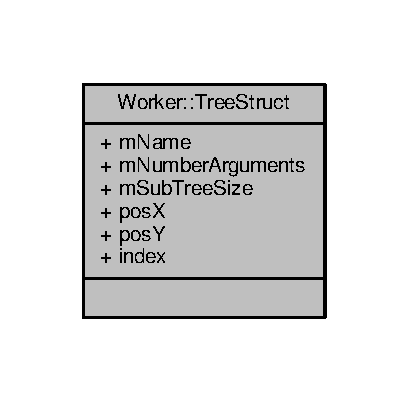
\includegraphics[width=196pt]{structWorker_1_1TreeStruct__coll__graph}
\end{center}
\end{figure}
\subsection*{Public Attributes}
\begin{DoxyCompactItemize}
\item 
\hypertarget{structWorker_1_1TreeStruct_acbf5cc3a0c62e30e99319f99cecf3ff2}{}Q\+Vector$<$ Q\+String $>$ {\bfseries m\+Name}\label{structWorker_1_1TreeStruct_acbf5cc3a0c62e30e99319f99cecf3ff2}

\item 
\hypertarget{structWorker_1_1TreeStruct_a134373fe62f1f9d100cbfade63f21542}{}Q\+Vector$<$ int $>$ {\bfseries m\+Number\+Arguments}\label{structWorker_1_1TreeStruct_a134373fe62f1f9d100cbfade63f21542}

\item 
\hypertarget{structWorker_1_1TreeStruct_a4800a5bcef2bd0805c2d56f5e78abbd0}{}Q\+Vector$<$ int $>$ {\bfseries m\+Sub\+Tree\+Size}\label{structWorker_1_1TreeStruct_a4800a5bcef2bd0805c2d56f5e78abbd0}

\item 
\hypertarget{structWorker_1_1TreeStruct_a4dc36aa9071b30cdeac0284c87081765}{}Q\+Vector$<$ float $>$ {\bfseries pos\+X}\label{structWorker_1_1TreeStruct_a4dc36aa9071b30cdeac0284c87081765}

\item 
\hypertarget{structWorker_1_1TreeStruct_a54a70132834e957ae4cb464fe0dd4a7c}{}Q\+Vector$<$ float $>$ {\bfseries pos\+Y}\label{structWorker_1_1TreeStruct_a54a70132834e957ae4cb464fe0dd4a7c}

\item 
\hypertarget{structWorker_1_1TreeStruct_ae0781ccbd9bb1677381f6bd003df2d0f}{}Q\+Vector$<$ int $>$ {\bfseries index}\label{structWorker_1_1TreeStruct_ae0781ccbd9bb1677381f6bd003df2d0f}

\end{DoxyCompactItemize}


The documentation for this struct was generated from the following file\+:\begin{DoxyCompactItemize}
\item 
source/worker.\+h\end{DoxyCompactItemize}

\hypertarget{classWorker}{}\section{Worker Class Reference}
\label{classWorker}\index{Worker@{Worker}}


Inheritance diagram for Worker\+:
\nopagebreak
\begin{figure}[H]
\begin{center}
\leavevmode
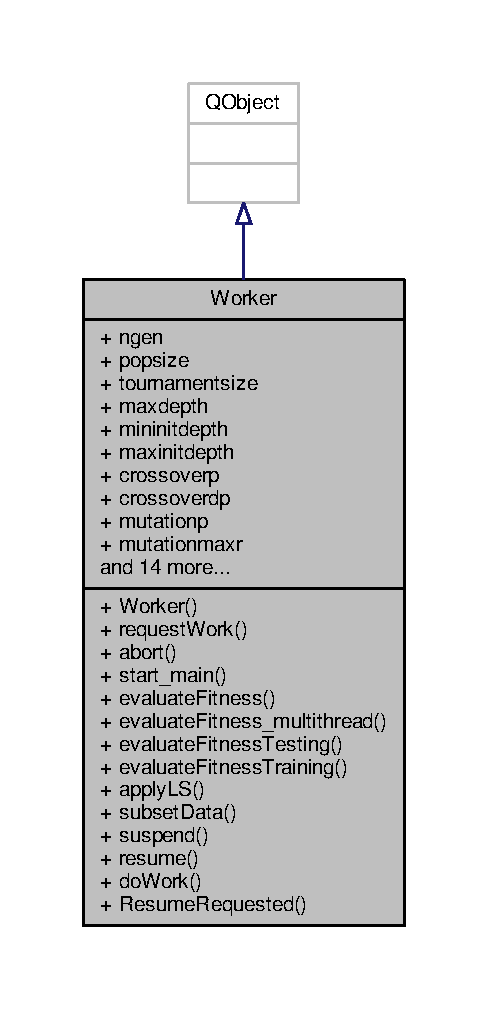
\includegraphics[width=234pt]{classWorker__inherit__graph}
\end{center}
\end{figure}


Collaboration diagram for Worker\+:
\nopagebreak
\begin{figure}[H]
\begin{center}
\leavevmode
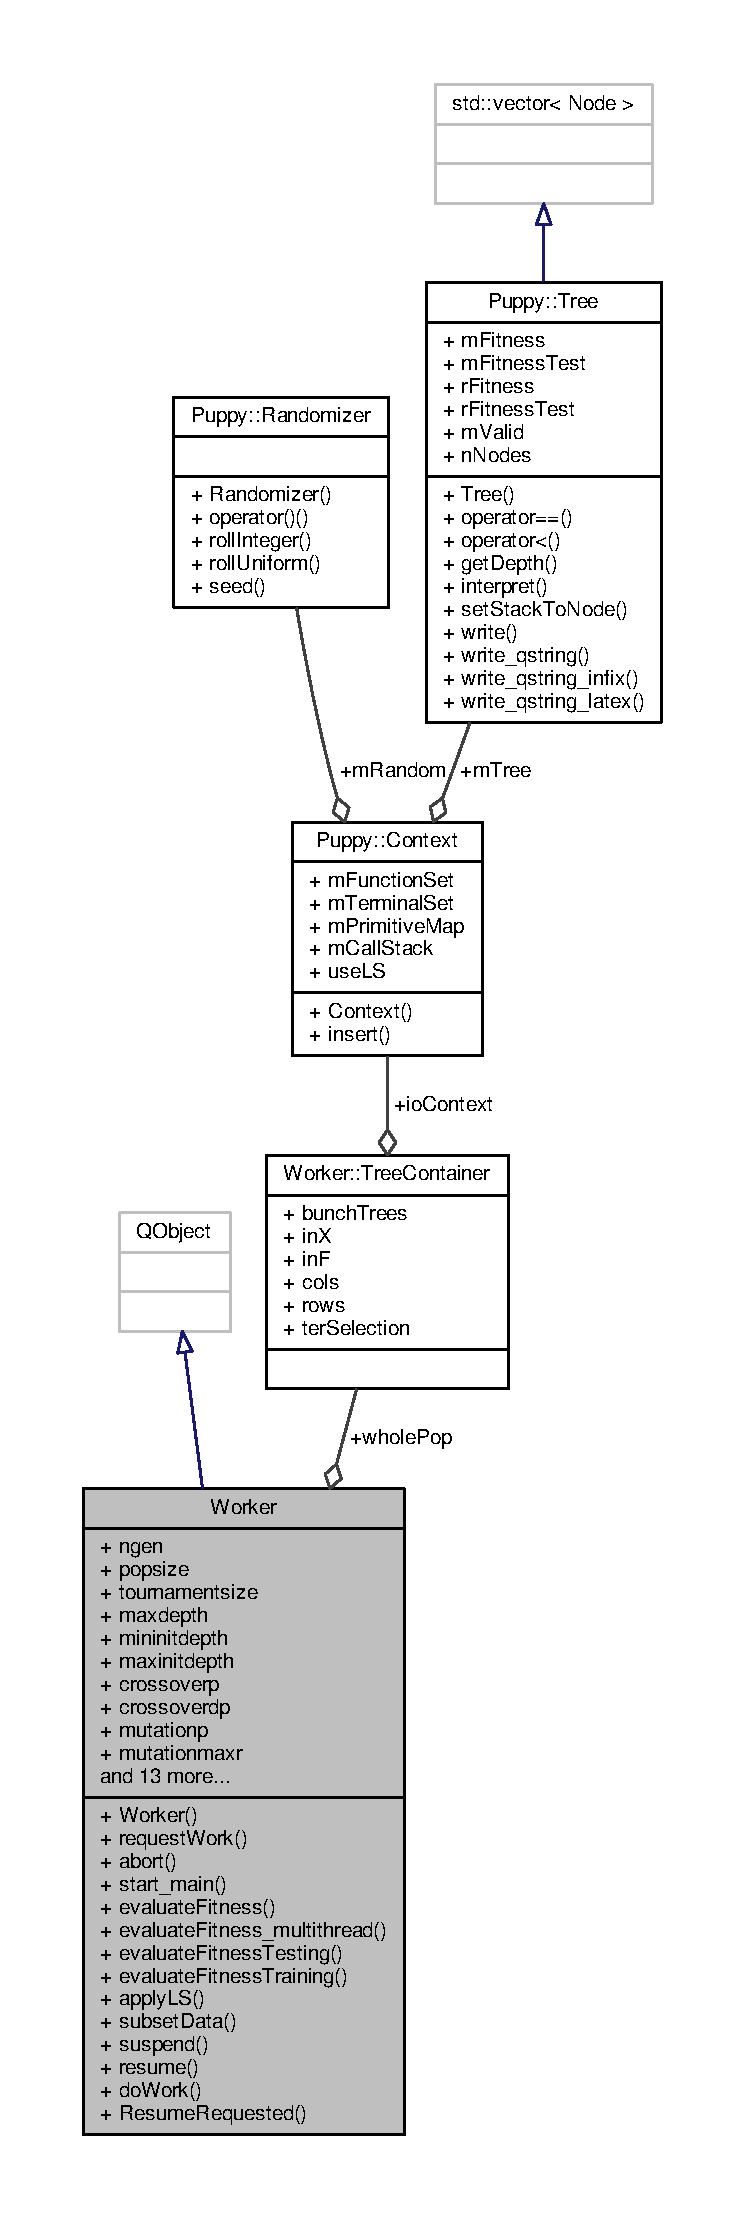
\includegraphics[height=550pt]{classWorker__coll__graph}
\end{center}
\end{figure}
\subsection*{Classes}
\begin{DoxyCompactItemize}
\item 
struct \hyperlink{structWorker_1_1fitnessdata}{fitnessdata}
\item 
struct \hyperlink{structWorker_1_1OneTree}{One\+Tree}
\item 
struct \hyperlink{structWorker_1_1Stats}{Stats}
\item 
struct \hyperlink{structWorker_1_1TreeContainer}{Tree\+Container}
\item 
struct \hyperlink{structWorker_1_1TreeStruct}{Tree\+Struct}
\end{DoxyCompactItemize}
\subsection*{Public Slots}
\begin{DoxyCompactItemize}
\item 
\hypertarget{classWorker_a4c6b6f22801862ae967df319161af625}{}void {\bfseries do\+Work} ()\label{classWorker_a4c6b6f22801862ae967df319161af625}

\item 
\hypertarget{classWorker_a2ef295af6e23dd8878f2427e4388591f}{}void {\bfseries Resume\+Requested} ()\label{classWorker_a2ef295af6e23dd8878f2427e4388591f}

\end{DoxyCompactItemize}
\subsection*{Signals}
\begin{DoxyCompactItemize}
\item 
\hypertarget{classWorker_ae4a138e6c8de2af5733d01024cd50ec6}{}void {\bfseries work\+Requested} ()\label{classWorker_ae4a138e6c8de2af5733d01024cd50ec6}

\item 
\hypertarget{classWorker_a30fe947e3103e2634af146469bd77db5}{}void {\bfseries value\+Changed} (const Q\+String \&value)\label{classWorker_a30fe947e3103e2634af146469bd77db5}

\item 
\hypertarget{classWorker_a91359586c82456b3c9d80d574137d7c4}{}void {\bfseries send\+\_\+stats} (\hyperlink{structWorker_1_1Stats}{Worker\+::\+Stats} data)\label{classWorker_a91359586c82456b3c9d80d574137d7c4}

\item 
\hypertarget{classWorker_a3732ec2fcbfcf0a51d455c7535d64bd1}{}void {\bfseries send\+\_\+stats\+\_\+end} (\hyperlink{structWorker_1_1Stats}{Worker\+::\+Stats} data)\label{classWorker_a3732ec2fcbfcf0a51d455c7535d64bd1}

\item 
\hypertarget{classWorker_a10bc16920395564f7051fa11993b9b32}{}void {\bfseries send\+\_\+tree} (\hyperlink{structWorker_1_1TreeStruct}{Worker\+::\+Tree\+Struct} data)\label{classWorker_a10bc16920395564f7051fa11993b9b32}

\item 
\hypertarget{classWorker_a55f2d2f20e208e3f7afd7ce74e241002}{}void {\bfseries progress\+Changed} (const int value)\label{classWorker_a55f2d2f20e208e3f7afd7ce74e241002}

\item 
\hypertarget{classWorker_af5db6a64c346ffc536852bdd4b907579}{}void {\bfseries G\+Pstarted} (const Q\+String value)\label{classWorker_af5db6a64c346ffc536852bdd4b907579}

\item 
\hypertarget{classWorker_a6f488c06d62e3ae49bd5af55fc0f7f90}{}void {\bfseries plot3\+D\+Send\+Data} (\hyperlink{structWorker_1_1fitnessdata}{Worker\+::fitnessdata} data)\label{classWorker_a6f488c06d62e3ae49bd5af55fc0f7f90}

\item 
\hypertarget{classWorker_ae713b051a9447d01ecdd4d6aef0eef9e}{}void {\bfseries send\+Eval\+Func} (unsigned long value)\label{classWorker_ae713b051a9447d01ecdd4d6aef0eef9e}

\item 
\hypertarget{classWorker_a8b434c0f74618a287aac3dd3de204618}{}void {\bfseries send\+\_\+tree\+\_\+string} (const Q\+String data)\label{classWorker_a8b434c0f74618a287aac3dd3de204618}

\item 
\hypertarget{classWorker_aadcaa7cdf5c014611db00b7e000868e5}{}void {\bfseries send\+\_\+tree\+\_\+infix\+\_\+string} (const Q\+String data)\label{classWorker_aadcaa7cdf5c014611db00b7e000868e5}

\item 
\hypertarget{classWorker_ae1dced9d9b9572d03d284a13638df49b}{}void {\bfseries send\+\_\+tree\+\_\+latex\+\_\+string} (const Q\+String data)\label{classWorker_ae1dced9d9b9572d03d284a13638df49b}

\item 
\hypertarget{classWorker_adfa119799838e68b671be5947a367f4a}{}void {\bfseries finished} ()\label{classWorker_adfa119799838e68b671be5947a367f4a}

\item 
\hypertarget{classWorker_a4cde48b2f055eb1f13546433a472a0d5}{}void {\bfseries request\+Fitness\+Calc} (const \hyperlink{structWorker_1_1TreeContainer}{Worker\+::\+Tree\+Container} data)\label{classWorker_a4cde48b2f055eb1f13546433a472a0d5}

\end{DoxyCompactItemize}
\subsection*{Public Member Functions}
\begin{DoxyCompactItemize}
\item 
\hypertarget{classWorker_a3290234525f8aad4f10f73305c9d1859}{}{\bfseries Worker} (Q\+Object $\ast$parent=0)\label{classWorker_a3290234525f8aad4f10f73305c9d1859}

\item 
\hypertarget{classWorker_a7def095438777bfa3c3b7adc3ada8481}{}void {\bfseries request\+Work} ()\label{classWorker_a7def095438777bfa3c3b7adc3ada8481}

\item 
\hypertarget{classWorker_a6ae95a49a7955d3efd052f27652c563a}{}void {\bfseries abort} ()\label{classWorker_a6ae95a49a7955d3efd052f27652c563a}

\item 
int \hyperlink{classWorker_a22bc35b7fff1c4cc8deb9a6b0a433c07}{start\+\_\+main} (void)
\begin{DoxyCompactList}\small\item\em Program main routine. \end{DoxyCompactList}\item 
\hypertarget{classWorker_a2c4efdf17d01c375f4aa390679827371}{}unsigned int {\bfseries evaluate\+Fitness} (std\+::vector$<$ \hyperlink{classPuppy_1_1Tree}{Puppy\+::\+Tree} $>$ \&io\+Population, \hyperlink{classPuppy_1_1Context}{Puppy\+::\+Context} \&io\+Context, double $\ast$in\+X, double $\ast$in\+F, int cols, int rows, std\+::vector$<$ bool $>$ \&ter\+Selection)\label{classWorker_a2c4efdf17d01c375f4aa390679827371}

\item 
\hypertarget{classWorker_af5bc25e98c2bb4d6aca90c1de5d3aa9b}{}unsigned int {\bfseries evaluate\+Fitness\+\_\+multithread} (std\+::vector$<$ \hyperlink{classPuppy_1_1Tree}{Puppy\+::\+Tree} $>$ \&io\+Population, \hyperlink{classPuppy_1_1Context}{Puppy\+::\+Context} \&io\+Context, double $\ast$in\+X, double $\ast$in\+F, int cols, int rows, std\+::vector$<$ bool $>$ \&ter\+Selection, bool multithread)\label{classWorker_af5bc25e98c2bb4d6aca90c1de5d3aa9b}

\item 
\hypertarget{classWorker_a8deae4f62f500e7f7ac353e2a46656f4}{}unsigned int {\bfseries evaluate\+Fitness\+Testing} (\hyperlink{classPuppy_1_1Tree}{Puppy\+::\+Tree} \&individual, \hyperlink{classPuppy_1_1Context}{Puppy\+::\+Context} \&io\+Context, double $\ast$in\+X, double $\ast$in\+F, int cols, int rows, std\+::vector$<$ bool $>$ \&ter\+Selection)\label{classWorker_a8deae4f62f500e7f7ac353e2a46656f4}

\item 
\hypertarget{classWorker_a26bc4ee37a10f29906f027d611985548}{}unsigned int {\bfseries evaluate\+Fitness\+Training} (\hyperlink{classPuppy_1_1Tree}{Puppy\+::\+Tree} \&individual, \hyperlink{classPuppy_1_1Context}{Puppy\+::\+Context} \&io\+Context, double $\ast$in\+X, double $\ast$in\+F, int cols, int rows, std\+::vector$<$ bool $>$ \&ter\+Selection)\label{classWorker_a26bc4ee37a10f29906f027d611985548}

\item 
\hypertarget{classWorker_a059d485ed0ff18bfcc245e03ae1f5af8}{}int {\bfseries apply\+L\+S} (\hyperlink{classPuppy_1_1Tree}{Puppy\+::\+Tree} \&individual, \hyperlink{classPuppy_1_1Context}{Puppy\+::\+Context} \&io\+Context, double $\ast$in\+X, double $\ast$in\+F, int cols, int rows, std\+::vector$<$ bool $>$ \&ter\+Selection, float \&ori\+Fit, float \&opt\+Fit)\label{classWorker_a059d485ed0ff18bfcc245e03ae1f5af8}

\item 
\hypertarget{classWorker_a6c8b8185bb9312134a86c1955f117890}{}void {\bfseries subset\+Data} (double $\ast$input, double $\ast$training, double $\ast$testing, int cols, int rows, int trainsize, int $\ast$index)\label{classWorker_a6c8b8185bb9312134a86c1955f117890}

\item 
\hypertarget{classWorker_a28d4ce0b0b8b86d4ab84d16c80770121}{}void {\bfseries suspend} ()\label{classWorker_a28d4ce0b0b8b86d4ab84d16c80770121}

\item 
\hypertarget{classWorker_a4e9811249da41dbc61677682b9e9a4ab}{}void {\bfseries resume} ()\label{classWorker_a4e9811249da41dbc61677682b9e9a4ab}

\end{DoxyCompactItemize}
\subsection*{Public Attributes}
\begin{DoxyCompactItemize}
\item 
\hypertarget{classWorker_ab2d9bc54fd2a6e31216acf5ac783347e}{}int {\bfseries ngen}\label{classWorker_ab2d9bc54fd2a6e31216acf5ac783347e}

\item 
\hypertarget{classWorker_a162442451cb8fb6a6044f0b71254836d}{}int {\bfseries popsize}\label{classWorker_a162442451cb8fb6a6044f0b71254836d}

\item 
\hypertarget{classWorker_a8a60bc5bf3119acbde4bca89dc3eea5d}{}int {\bfseries tournamentsize}\label{classWorker_a8a60bc5bf3119acbde4bca89dc3eea5d}

\item 
\hypertarget{classWorker_a3b1a8d57d8b0f280dbdf818d38a53168}{}int {\bfseries maxdepth}\label{classWorker_a3b1a8d57d8b0f280dbdf818d38a53168}

\item 
\hypertarget{classWorker_a6278941636091560e37bdb753e53611b}{}int {\bfseries mininitdepth}\label{classWorker_a6278941636091560e37bdb753e53611b}

\item 
\hypertarget{classWorker_a37ec4012eddf63f76a0eb3166b32e923}{}int {\bfseries maxinitdepth}\label{classWorker_a37ec4012eddf63f76a0eb3166b32e923}

\item 
\hypertarget{classWorker_acaeca7f4f5a924a388b403454fd98b35}{}float {\bfseries crossoverp}\label{classWorker_acaeca7f4f5a924a388b403454fd98b35}

\item 
\hypertarget{classWorker_aec28e1605cef6d1e1916bdb84fb9249b}{}float {\bfseries crossoverdp}\label{classWorker_aec28e1605cef6d1e1916bdb84fb9249b}

\item 
\hypertarget{classWorker_a7e81ba98fd648c243f5e227656d42eea}{}float {\bfseries mutationp}\label{classWorker_a7e81ba98fd648c243f5e227656d42eea}

\item 
\hypertarget{classWorker_aebaeae53537a9336e11c9c5a2a961ea6}{}int {\bfseries mutationmaxr}\label{classWorker_aebaeae53537a9336e11c9c5a2a961ea6}

\item 
\hypertarget{classWorker_a4c0c7f0dc25095839a4e761568d6e6c1}{}int {\bfseries randomseed}\label{classWorker_a4c0c7f0dc25095839a4e761568d6e6c1}

\item 
\hypertarget{classWorker_a64bf5d8f1d9350b70d366e6a43c39fba}{}double $\ast$ {\bfseries dataset}\label{classWorker_a64bf5d8f1d9350b70d366e6a43c39fba}

\item 
\hypertarget{classWorker_a05ea9a7a069322b5cd3b80d7c955f1c0}{}int {\bfseries dataset\+\_\+cols}\label{classWorker_a05ea9a7a069322b5cd3b80d7c955f1c0}

\item 
\hypertarget{classWorker_acbe8642cda2ebfec7cedbd329892e9bf}{}int {\bfseries dataset\+\_\+rows}\label{classWorker_acbe8642cda2ebfec7cedbd329892e9bf}

\item 
\hypertarget{classWorker_aa832f7af255998292b58f2c6dfb6718e}{}double $\ast$ {\bfseries dataset\+\_\+training}\label{classWorker_aa832f7af255998292b58f2c6dfb6718e}

\item 
\hypertarget{classWorker_a4692da54491abf6c8119adae498aff57}{}double $\ast$ {\bfseries dataset\+\_\+testing}\label{classWorker_a4692da54491abf6c8119adae498aff57}

\item 
\hypertarget{classWorker_aa882edd61d31c3d15e6737f54f804f4a}{}int {\bfseries training\+P}\label{classWorker_aa882edd61d31c3d15e6737f54f804f4a}

\item 
\hypertarget{classWorker_a7dd1dfdc0a74074c82efa5f0d7c32a1e}{}bool {\bfseries L\+Sactivated}\label{classWorker_a7dd1dfdc0a74074c82efa5f0d7c32a1e}

\item 
\hypertarget{classWorker_a34fec1328c31ba6e844a9a93c8f7cae2}{}bool {\bfseries multicore\+\_\+activated}\label{classWorker_a34fec1328c31ba6e844a9a93c8f7cae2}

\item 
\hypertarget{classWorker_a70ec9cce22a12a9d582a3596fef6fbf4}{}std\+::vector$<$ bool $>$ {\bfseries terminalselection}\label{classWorker_a70ec9cce22a12a9d582a3596fef6fbf4}

\item 
\hypertarget{classWorker_a9dc8e869da4a241ee0bda2e10d2259e5}{}std\+::vector$<$ bool $>$ {\bfseries functionselection}\label{classWorker_a9dc8e869da4a241ee0bda2e10d2259e5}

\item 
\hypertarget{classWorker_a028b694c257b109a56a1fa11cc067cad}{}Q\+Vector$<$ \hyperlink{classPuppy_1_1Tree}{Puppy\+::\+Tree} $>$ {\bfseries fitness\+Valid}\label{classWorker_a028b694c257b109a56a1fa11cc067cad}

\item 
\hypertarget{classWorker_a63db29e69c7054d2084f3d51981a390e}{}bool {\bfseries fitness\+Valid\+Finished}\label{classWorker_a63db29e69c7054d2084f3d51981a390e}

\item 
\hypertarget{classWorker_a7ccf6daed284312665431edfb1378d53}{}\hyperlink{structWorker_1_1TreeContainer}{Tree\+Container} {\bfseries whole\+Pop}\label{classWorker_a7ccf6daed284312665431edfb1378d53}

\end{DoxyCompactItemize}


\subsection{Member Function Documentation}
\hypertarget{classWorker_a22bc35b7fff1c4cc8deb9a6b0a433c07}{}\index{Worker@{Worker}!start\+\_\+main@{start\+\_\+main}}
\index{start\+\_\+main@{start\+\_\+main}!Worker@{Worker}}
\subsubsection[{start\+\_\+main}]{\setlength{\rightskip}{0pt plus 5cm}int Worker\+::start\+\_\+main (
\begin{DoxyParamCaption}
\item[{void}]{}
\end{DoxyParamCaption}
)}\label{classWorker_a22bc35b7fff1c4cc8deb9a6b0a433c07}


Program main routine. 


\begin{DoxyParams}{Parameters}
{\em argc} & Number of arguments given on the command-\/line. \\
\hline
{\em argv} & Command-\/line arguments. \\
\hline
\end{DoxyParams}


The documentation for this class was generated from the following files\+:\begin{DoxyCompactItemize}
\item 
source/worker.\+h\item 
source/main\+G\+P.\+cpp\item 
source/worker.\+cpp\end{DoxyCompactItemize}

%--- End generated contents ---

% Index
\backmatter
\newpage
\phantomsection
\clearemptydoublepage
\addcontentsline{toc}{chapter}{Index}
\printindex

\end{document}
